%# -*- coding: utf-8-unix -*-
% !TEX program = xelatex
% !TEX root = ../thesis.tex
% !TEX encoding = UTF-8 Unicode
%%==================================================
%% chapter01.tex for SJTU Master Thesis
%%第四章
%%==================================================
\chapter{基于深度强化学习的一对一及多对多博弈策略}
\section{引言}
在上一章主要以双人棋盘类博弈策略进行描述,在本章将讨论非棋盘类单智能体对抗和多智能体对抗的问题。对于对称类棋盘游戏来说,其规则简单,并且可落子范围随着双方不断落子逐渐缩小,当棋盘全部走满双方平局,也就是动作双方最多走满全盘步数即可或胜负,应用场景比较单一,对于其他应用场景还有待扩展,除此之外,现有的强化学习模型大多数针对单智能体游戏类的决策任务,对于多智能体强化学习的扩展还有待发掘。原因是当对多智能体进行建模时,每一个智能体不仅需要感知外界环境,同时也需要及时获得其他智能体的信息,其他智能体进行动作可能会影响整个环境状态的变化,因此对于多智能体其动作空间和环境状态空间增大带来训练的困难。根据智能体之间的关系可以分为合作,竞争和既有竞争又有合作,对于这种比较复杂的模型,奖励的分配也是面临的难题之一。本章将介绍多智能体强化学习相关的理论算法基础后,设计一对一智能体相互对抗的实验场景,根据实际情况建立合理的状态动作以及奖励函数,并把实验场景拓展到多对多上,接着展示实验结果并进行分析。
\section{多智能体强化学习理论基础}
在多智能体研究中,智能体之间的关系可以是合作的、竞争的,也可以是两者兼而有之,许多算法都是为智能体特定的关系设立的。
如\cite{Lazaridou2017Multi}主要针对多智能体合作问题提出的,基于假设所有智能体的行为都是在提高集体奖励的基础上进行的。另一种方式是通过共享参数达到合作的目的\ref{Gupta2017Cooperative},这需要所有的智能体模型都相同,奖励也相同。这些算法一般不适用于竞争环境或混合环境。本章将就单智能体间的相互对抗拓展到多智能体间的组队形式的对抗,也就是同队之间智能体是相互协作的,异队间智能体是相互对抗的,所有智能体的优化目标都是降低敌方奖励,增加本方奖励。
下面介绍常用的多智能体强化学习算法。
\subsection{Minimax-Q学习}
Minimax-Q\cite{Littman1994Markov}是一种适用于双人零和博弈的算法。其主要思想是两个智能体之间的奖励函数是互为相反数的,一方利益的最小化同时是另一方利益的最大化,所以两个智能体之间可以共享一个相同的奖励函数,是基于Q-learning算法进行实现的,Minimax—Q学习的值函数是Q值矩阵的最小最大化:
\begin{equation}
{{\rm{V}}^1}{\rm{(s) = }}\mathop {\max }\limits_{{\pi ^1} \in PD({A^1})} \mathop {\min }\limits_{{a^2} \in {A^2}} \sum\limits_{{a^1} \in {A^1}} {{Q_t}^1(s,{a^1},{a^2})} {\pi ^1}
\end{equation}
其中,${\pi ^1}$为第一个智能体的策略,在状态$S$下,当已知第二个智能体采取动作$a_2$,第一个智能体采取动作$a_1$时,其$Q$值函数为:

\begin{equation}
\begin{aligned}
Q_{t + 1}^1(s,{a^1},{a^2}) =& (1 - {\alpha _t})Q_t^1(s,{a^1},{a^2}) + {\alpha _t}[R_t^1(s,{a^1},{a^2}) \\& + \gamma\mathop {\max }\limits_{{\pi ^1} \in PD({A^1})} \mathop {\min }\limits_{{a^2} \in {A^2}} \sum\limits_{{a^1} \in {A^1}} {{Q_t}^1(s,{a^1},{a^2})} {\pi ^1} ]
\end{aligned}
\end{equation}
Minimax-Q学习具有很好的收敛性,但是适用场景相对单一只适用于两人零和博弈,不能应用于多智能体的协作和对抗。
\subsection{Nash-Q学习}
Nash-Q学习改进了Minimax——Q学习中对于零和博弈的局限,主要针对非零和的情况,其认为智能体最后的最优Q函数可以用Nash平衡解定义。假设所有智能体在某一状态$s$下的$Nash$平衡解为${\pi ^1}(s),...,{\pi ^n}(s)$,则第$i$个智能体的值函数定义为:
\begin{equation}
	{V^i}(s) = NashQ_t^i(s) = {\pi ^1}(s)...{\pi ^n}(s)Q_t^i(s)
\end{equation}
所以Nash—Q学习中Q值的更新规则为:
\begin{equation}
Q_{t + 1}^1(s,{a^1},...,{a^n}) = (1 - {\alpha _t})Q_t^1({\rm{s}},{a^1},...,{a^n}) + {\alpha _t}[r_t^1 + \gamma NashQ_t^i(s')]
\end{equation}
当其他智能体进行动作更新时,当前智能体需要不断维护自己的Q值函数。这样计算的复杂度大大增加,同时如何寻求Nash解也是Nash—Q算法面临的困难。
\subsection{Friend-or-Foe Q 学习}
Friend-or-Foe Q 学习把合作和竞争整合到了一个框架下,当对方是Friend时,智能体的个体利益和系统整体利益一致:
\begin{equation}
NashQ_t^i(s) = \mathop {\max }\limits_{{a^1} \in {A^1},{a^2} \in {A^2}} Q_t^1(s,{a^1},{a^2})
\end{equation}
当对方是Foe时,对策变为零和博弈:
\begin{equation}
	NashQ_t^i(s) = \mathop {\max }\limits_{{\pi ^1} \in PD({A^1})} \mathop {\min }\limits_{{a^2} \in {A^2}} \sum\limits_{{a^1} \in {A^1}} {\pi ({a^1})} Q_t^1(s,{a^1},{a^2})
\end{equation}

该算法存在一个问题是需要指定每个智能体和当前智能体的关系,并且要把智能体提前进行划分,每个智能体只具有个体能力不具有全局感知能力。
\section{基于AC框架下的多智能体强化学习}
前面所述经典的多智能体算法都是基于Q值学习进行策略更新的。当其他智能体进行动作时,需要不断更新当前智能体的Q值函数表,同时奖励的分配也是需要加规则进行干预的。这里考虑用AC框架进行多智能体强化学习的研究。奖励不需要人为分配,通过Critic函数告诉Actor当前动作的得分,对于一个有$N$个智能体的博弈环境,假设其策略梯度的参数为$\theta  = \{ {\theta _1},...{\theta _N}\} $,其策略的集合为$\pi  = \{ {\pi _1},...{\pi _N}\} $,对于第$i$个智能体,其期望收益的梯度$J({\theta _i}) = E[{R_i}]$为:
\begin{equation}
	{\nabla _{{\theta _i}}}J({\theta _i}) = {E_{s \sim {p^u},{a_i} \sim {\pi _i}}}[{\nabla _{{\theta _i}}}\log {\pi _i}({a_i}|{o_i}){Q_i}^\pi ({a_i},...{a_N})]
\end{equation}
${\nabla _{{\theta _i}}}J({\theta _i}) = {E_{s \sim {p^u},{a_i} \sim {\pi _i}}}[{\nabla _{{\theta _i}}}\log {\pi _i}({a_i}|{o_i}){Q_i}^\pi ({a_i},...{a_N})]$
其中${Q_i}^\pi ({a_i},...{a_N})$是将所有智能体的动作信息作为输入,对当前智能体的期望收益作为输出的打分函数。对于每一个智能体都有自己的奖励函数结构,因此这个打分函数可以学习到合作和竞争混合的结构。经验池中存储了每一个智能体的观测状态,动作信息和奖励$(x,{a_1},...{a_N},{r_1},...,{r_N})$,
对于每一个智能体,其策略梯度函数的更新方式为:
\begin{equation}
	L({\theta _i}) = {E_{x,a,r,x'}}[{({Q_i}^u(x,{a_1},...,{a_N}) - y)^2}]
\end{equation}

其中$y = {r_i} + \gamma {Q_i}^{u'}(x',{a_1}^\prime ,...,{a'_N}){|_{{{a'}_j} = {{u'}_j}({o_j})}}$
这里$u' = \{ {u_{{{\theta '}_1}}},...,{u_{{{\theta '}_N}}}\} $是当其他智能体进行动作后新的策略。



当利用AC模型进行建模时,对于一对一智能体的网络结构,Actor网络和Critic网络是特征输入平面是相同的,都是把当前棋局作为原始输入,因此可以采用相同的深度学习网络进行特征提取,由于动作策略网络Actor输出的是概率值,Critic网络输出的是评分,在提取特征后可以把网络分成两部分,训练时,Actor根据当前的state选择一个Action,然后Critic可以根据state-action计算一个Q值,作为对Actor动作的反馈。Critic根据估计的Q值和实际的Q值来进行训练,Actor根据Critic的反馈来更新策略。测试时,我们只需要Actor就可以完成,此时不需要Critic的反馈。对于多对多智能体作战而言,对于每个智能体不仅要考虑到敌方智能体的位置,还要考虑我方其他智能体的状态。每个Agent的训练同单个智能体对抗算法的训练过程类似,不同的地方主要体现在Critic的输入上:在单个Agent的算法中,Critic的输入是一个state-action对信息,但是在多对多智能体中,每个Agent的Critic输入除自身的state-action信息外,还可以有额外的信息,比如其他Agent的动作。


\section{一对一单智能体场景设计}
\subsection{问题描述}
首先从单智能体入手,进行问题描述和建模。这里我们设计了一个吃小鱼游戏。
游戏的规则如下:在10*10的网格里,左下角和右上角红蓝两方各有一个智能体,进行相互博弈。红蓝两方交替进行移动,直到一方被另一方吃掉。这里面有两个概念:追击角和逃逸角。红方对蓝方的追击角为红方速度方向和红蓝两方质心连线的夹角。蓝方的逃逸角为蓝方速度方向和蓝方到红方质心连线的夹角。如图\ref{zhuijijiao}所示。
\begin{figure}[!htp]
	\centering
	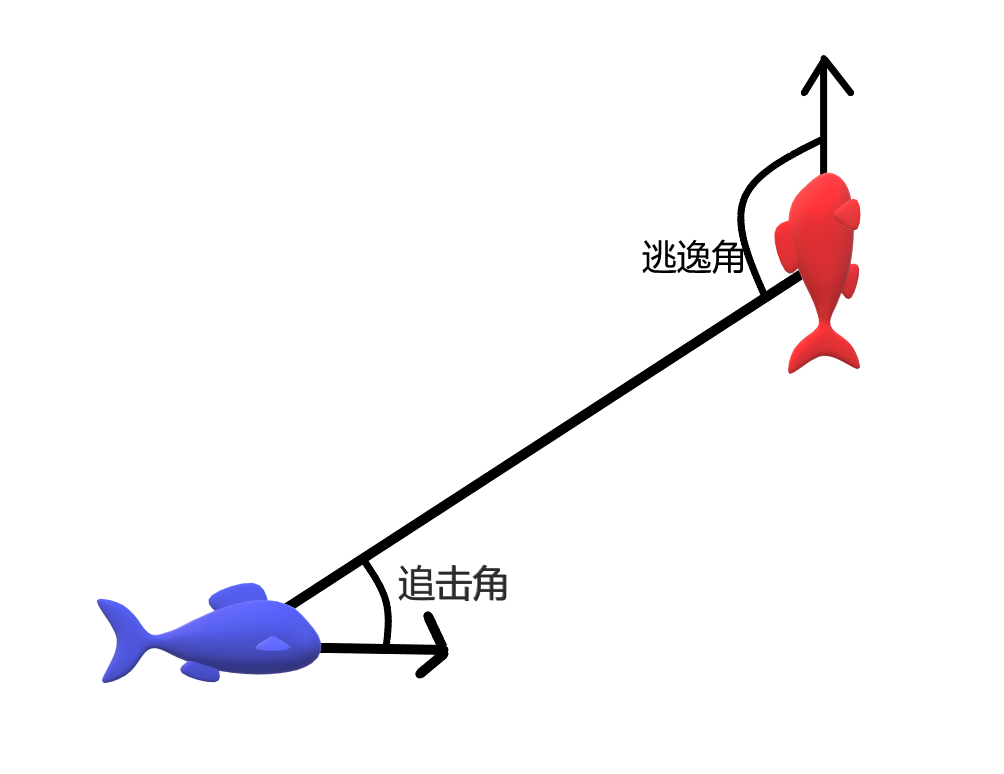
\includegraphics[width=10cm]{example/zhuijijiao.png}
	\bicaption[这里将出现在插图索引]
	{追击角和逃逸角示意图}
	{Neural network training pipeline}
	\label{fig:zhuijijiao}
\end{figure}
红方吃掉蓝方的规则如下:红方到蓝方距离小于四个单位长度,红方的追击角小于30度,蓝方的逃逸角大于30度。反之蓝方对红方追击角小于30度,红方逃逸角大于30度,蓝方吃掉红方。最后留下的一方获胜。
\subsection{场景建模}
在强化学习框架下,需要对状态空间,动作空间以及奖励函数进行合理表示。对于深度学习部分,需要设计状态空间特征提取的网络结构,以及网络输出的维度和激活函数和损失函数。这里采用蒙特卡洛搜索树进行建模,需要把强化学习思想映射到蒙特卡洛搜索树的结构上,包括根节点和分支包含的信息以及叶子节点返回的值。
首先从游戏规则考虑,游戏获胜的条件和速度方向以及双方的位置信息有关,所以特征平面需要涵盖相关信息,在这里选择5层的10*10的特征空间表示状态信息,第一层为我方当前的位置,第二层为我方上一步的位置,第三层为敌方当前位置,第四层为敌方上一步位置,第五层用来表示我方是红方还是蓝方,红方为全0,蓝方为全1。在动作选择上,由于移动的位置只能是相连的上下左右四个方向,所以动作空间为4个离散的值,0代表向上移动,1代表向下移动,2代表左,3代表右,返回的奖励函数为获胜一方的奖励为1,失败一方奖励为-1。由于小鱼走过的位置还可以重复走,所以这里设置为当两方各自走过的步数超过200步还没有分出胜负,判定为平局,奖励为0。
当每进行一次动作选择,对当前状态进行400次蒙特卡洛树搜索统计搜索结果。根据每个节点的访问次数利用式\ref{eq:gailu}和\ref{eq:zaosheng}进行节点信息统计得到当前状态的动作这里面选取温度常数$\tau=1$,噪声系数$\varepsilon=0.25$。在每一次蒙特卡洛树的搜索和建立中,对于当前位置可选的动作有上下左右,当智能体在围墙边界时,会把不能移动的动作去掉,根据可行动作进行树的节点扩展。对于当前智能体的子节点扩展就是对方可行的动作。在动作选择时,选取最大的$Q+U$进行动作的选择,这里$Q$代表经过当前节点获得的平均奖励,$U$为根据深度学习网络得到的先验概率。



\section{多对多智能体场景设计}

\subsection{问题描述}
本节在上一节的基础上,由一对一智能体之间的相互博弈拓展到多对多智能体的相互博弈。被吃掉的规则和上一节相同。这里红方蓝方各有两个小鱼,分别在左下角和右上角,给两方小鱼一个初始速度和位置,游戏规则如下:四个小鱼轮流进行移动,移动的范围是上下左右,当下一动作撞到墙壁或本方队友时,认为该动作是非法的。红色和粉色的小鱼为一队,浅蓝色和深蓝色小鱼为一队,行动的顺序为红,深蓝,粉,浅蓝。四个小鱼初始位置如图\ref{小鱼初始位置}。

\begin{figure}[!htbp]
	\centering
	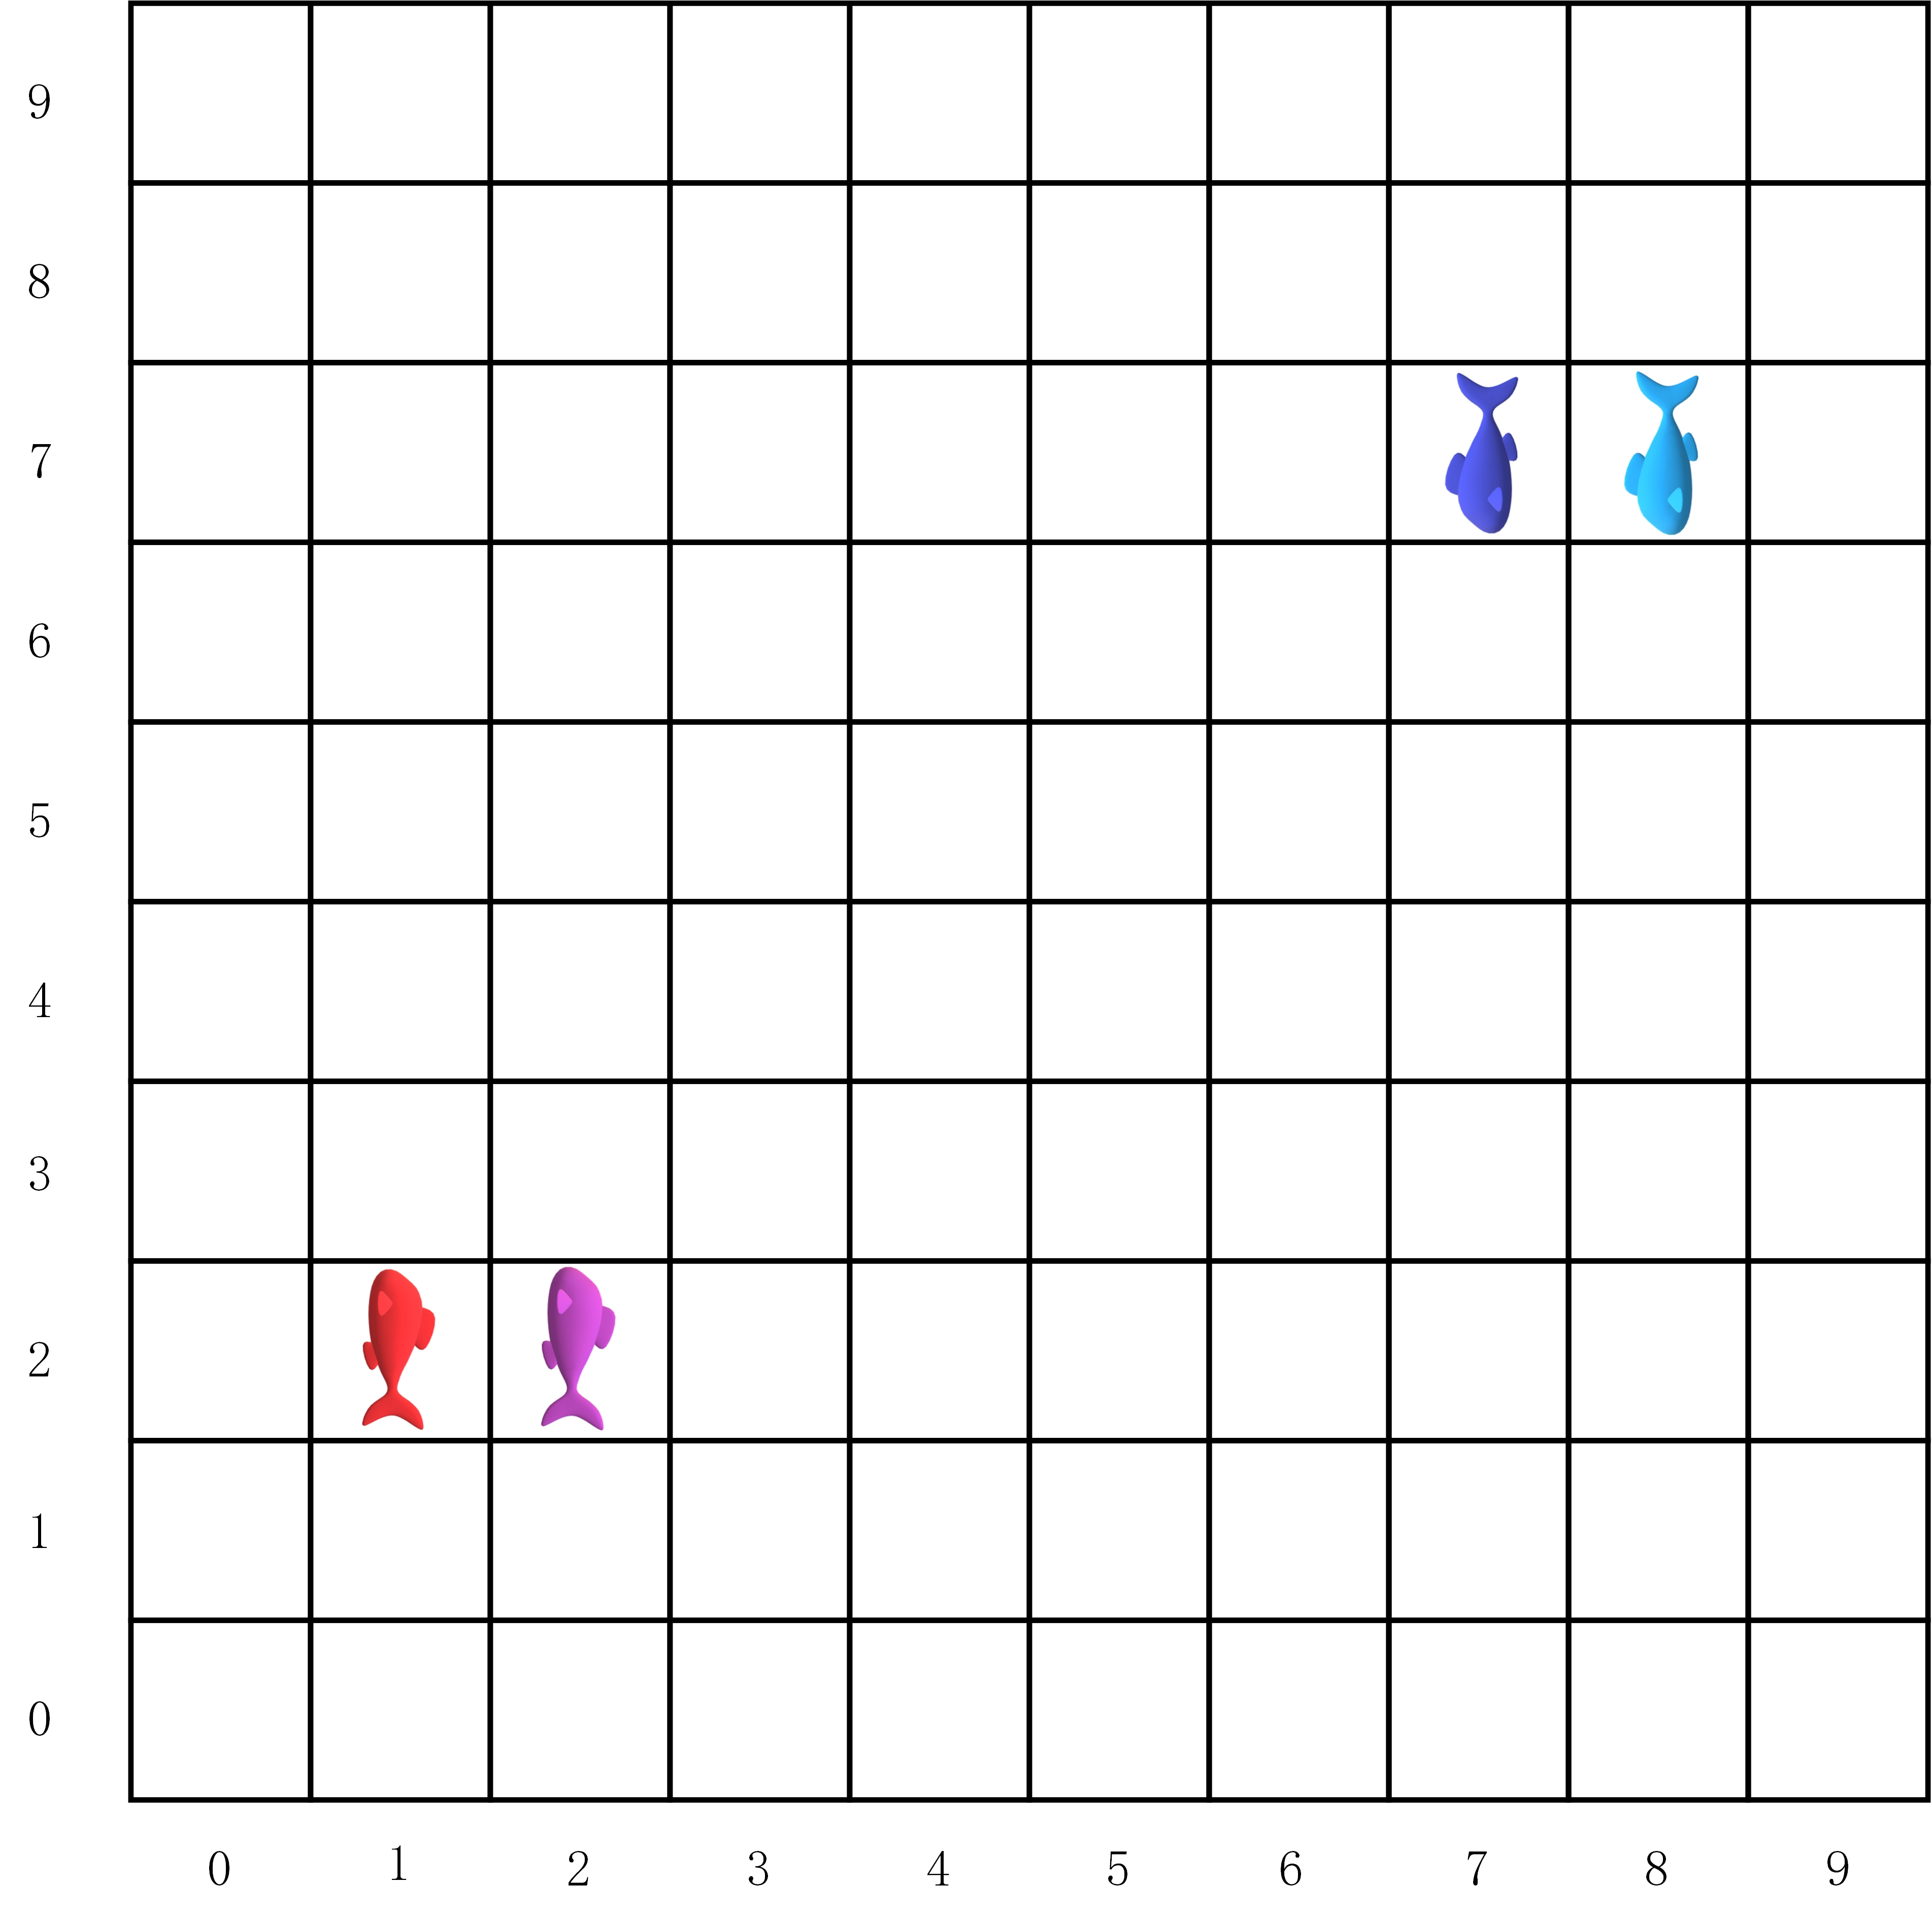
\includegraphics[width=\hsize]{example/xiaoyuchushiweizhi.jpg}
	\bicaption[这里将出现在插图索引]
	{小鱼初始位置示意图}
	{The Diagrammatic Drawing of Minmax Search Tree}
	\label{小鱼初始位置}
\end{figure}

给红色小鱼初始位置为(1,2)初速度为向上,粉色小鱼初始位置为$(2,2)$初速度为向上,深蓝色小鱼初始位置为(7,7),浅蓝色小鱼初始位置为$(8,7)$,初速度都为向下。游戏结束的规则为当有任意一条小鱼被吃掉,该方判为输家。因此整个游戏的流程为:

\begin{algorithm}[!htbp]
	\caption{多对多游戏流程}% Ëã·¨±êÌâ
	\begin{algorithmic}[1]%Ò»ÐÐÒ»¸ö±êÐкÅ
		\For{每个智能体移动的次数不超过移动步数上限 }
		\State 红色小鱼根据强化学习策略从合法动作中选择一个进行动作
		\State 判断红色小鱼和对方两条小鱼的状态关系
		\If {任意一条小鱼被吃掉}
		\State 游戏结束,跳出循环,返回结果
		\EndIf
		\State 蓝色小鱼根据强化学习策略从合法动作中选择一个进行动作
		\State 判断蓝色小鱼和对方两条小鱼的状态关系
		\If {任意一条小鱼被吃掉}
		\State 游戏结束,跳出循环,返回结果
		\EndIf
		\State 粉色小鱼根据强化学习策略从合法动作中选择一个进行动作
		\State 判断粉色小鱼和对方两条小鱼的状态关系
		\If {任意一条小鱼被吃掉}
		\State 游戏结束,跳出循环,返回结果
		\EndIf
		\State 浅蓝色小鱼根据强化学习策略从合法动作中选择一个进行动作
		\State 判断浅蓝色小鱼和对方两条小鱼的状态关系
		\If {任意一条小鱼被吃掉}
		\State 游戏结束,跳出循环,返回结果
		\EndIf
		
		\EndFor
	\end{algorithmic}
\end{algorithm}
\subsection{场景建模}
在多对多场景中,相当于每个智能体不仅需要感知当前状态,还需要感知本方智能体和敌方智能体所有的动作信息。智能体的动作可以通过上一步的位置和当先位置得到,所以在本实验中状态设置为10*10*9。与上一节一样,10*10代表棋盘大小,第一层是红色小鱼当前位置,第二层为红色小鱼上一步位置,第三层第四层依次表示粉色小鱼信息,第五,六层为蓝色小鱼信息,第七,八层为浅蓝色小鱼信息,第九层带表当前训练的是哪个智能体。
由于设计的状态包含了当前环境状态和其他智能体的动作信息,在利用深度学习网络拟合值函数和策略函数时,特征提取部分的网络结构可以共享,深度学习网络结构如下图所示:

\begin{figure}[!htpb]
	\centering
	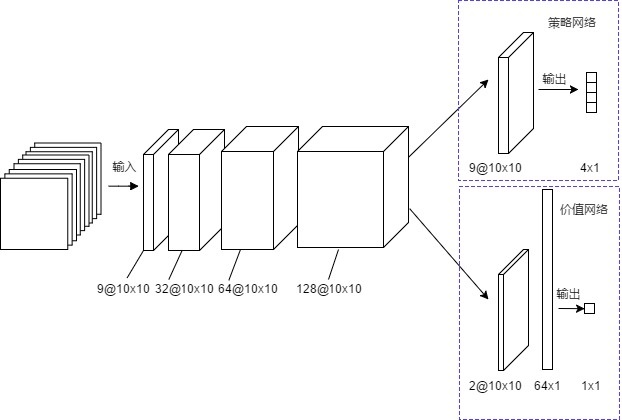
\includegraphics[width=10cm]{example/wangluojiegoutu.jpg}
	\bicaption[这里将出现在插图索引]
	{多对多深度学习网络结构图}
	{Neural network training pipeline}
	\label{fig:wangluojiegoutu}
\end{figure}

多对多强化学习博弈算法流程图为:
\begin{algorithm}[!htbp]
	\caption{多对多强化学习博弈算法}% Ëã·¨±êÌâ
	\begin{algorithmic}[1]%Ò»ÐÐÒ»¸ö±êÐкÅ
		\Require
		包含当前位置和历史走过位置的状态信息,游戏动作规则,游戏奖励规则。随机初始化神经网络的参数$\theta_0$
		\Ensure 
		动作策略$p$,状态价值$v$
		\For{每一次迭代$iteration=1$ to $T$ }
		 \If{达到下列之一终止条件:
		 \begin{enumerate}
		     	 \item 所有智能体都没有可选动作
		     	 \item 达到了游戏最大的行动数还没分出胜负
	     \end{enumerate}}
		\State 跳出当前循环
		\Else
		\State 继续进行本次循环
		\EndIf
		\State 初始化状态$S_0$
		\For {对于在$t$时刻的动作}
		\State 利用$MCTS$算法进行搜索
		\While{$MCTS$搜索次数小于$n_playout$}
		\State 进行树节点的选择:每次模拟通过选择最大上限置信度$Q(s,a)+U(s,a)$进行树的遍历。这里${\rm{U}}(s,a) \propto P(s,a)/(1 + N(s,a))$
		\State 叶节点的扩展和状态值评估:
		利用神经网络计算结果进行叶节点展开和对应状态值的评估。$(P(s, \cdot ),V(s)) = {f_{{\theta _i}}}(s)$,$p$值的向量存储在从$s$输出的边中。
		\State 回溯:
		当进行树的模拟遍历时,被访问的边会进行相应的节点访问次数更新,$Q(s,a) = 1/N(s,a)\sum\nolimits_{s'|s,a \to s'} {V(s')} $,这里${s'|s,a \to s'}$代表在状态$s$采取动作$a$后到达状态$s'$。
		\EndWhile
		\State 动作选择:
		\\当搜索结束后,根据搜索的结果根据式\ref{eq:gailu}结合温度参数统计每个动作被访问的概率。根据得到的结果选择一个动作进行到下一状态$s_t+1$的转移。
		\EndFor
		  \algstore{MergeSort}
		\end{algorithmic}
		\end{algorithm}

		\begin{algorithm}[!htbp]
		\begin{algorithmic}[1]
		\algrestore{MergeSort}
		\State 记录当前幕中经过的所有的状态和最后游戏的结果${r_T} \in \{  - 1, + 1\} $
		\For{在得到最后的获胜结果后,对于之前走过的每一步}
		\State 从当前玩家角度更新最后游戏的得分${z_t} \leftarrow  \pm {r_T}$,结合之前保存的每一步状态,存储数据的格式为$s_t,\pi_t,z_t$
		\EndFor
		\State 对于最新模型self-play产生的数据进行随机采样。
		\State 通过以下损失函数:
		\begin{equation}
		l = {(z - v)^2} - {\pi ^T}\log p + c||{\theta _i}{\rm{|}}{{\rm{|}}^{\rm{2}}}
		\end{equation}
		最大化策略网络输出的概率分布和蒙特卡洛搜索树得到的概率之间的相似度,同时最小化价值函数的预测得分和$self-play$得到的最后结果之间的误差。
		调整输入给蒙特卡洛树的神经网络参数$(p,v) = {f_{{\theta _i}}}(s)$。
		\If {$iteration\%check_point==0$}
		\State 利用最新数据训练出来的模型(参数为$\theta '$)和之前最好的模型(参数为$\theta$)进行对弈
		\If {获胜率大于0.8}
		 \State 进行网络参数更新${\theta _{i + 1}} = \theta '$,用于下一次$self-play$数据生成中的先验概率。
		\Else
		 \State 不进行网络参数更新,${\theta _{{\rm{i + 1}}}}{\rm{ = }}\theta $
		\EndIf
		\EndIf
		\EndFor
	\end{algorithmic}
\end{algorithm}

从上述算法可以看出,$MCTS$可以看作是一个策略改进的实现,$MCTS$在深度学习输出的先验概率${f_{{\theta _{i - 1}}}}$基础上搜索策略${\pi _t} = {\alpha _{{\theta _{i - 1}}}}({s_t})$。树的边建立了一系列状态动作对$(s,a)$,记录了先验概率$P(s,a)$,节点访问次数$N(s,a)$和状态动作值$Q(s,a)$。$self-play$的过程可以看作策略迭代网络的标签数据,在每一次自我博弈中,选择获胜玩家的数据进行一个正样本。训练深度学习网络权重${\theta _i}$,价值网络损失函数为回归常用的均方误差${(z - v)^2}$,策略网络为交叉熵$ - {\pi ^T}\log p$。这里同时训练两个网络所以将两项目标函数进行加和,利用梯度下降法进行网络参数的更新。

\section{实验结果与分析}

\subsection{一对一实验结果}
在一对一实验中,给红蓝两方一个初始位置分别为$(2,3)$和$(7,7)$,红方初速度为向上,蓝方初速度为向下。这里人控制红方,蓝方为学习到的智能体模型。红蓝两方的初始状态如图\ref{yiduiyi1.jpg}:
\begin{figure}[!hbtp]
	\centering
	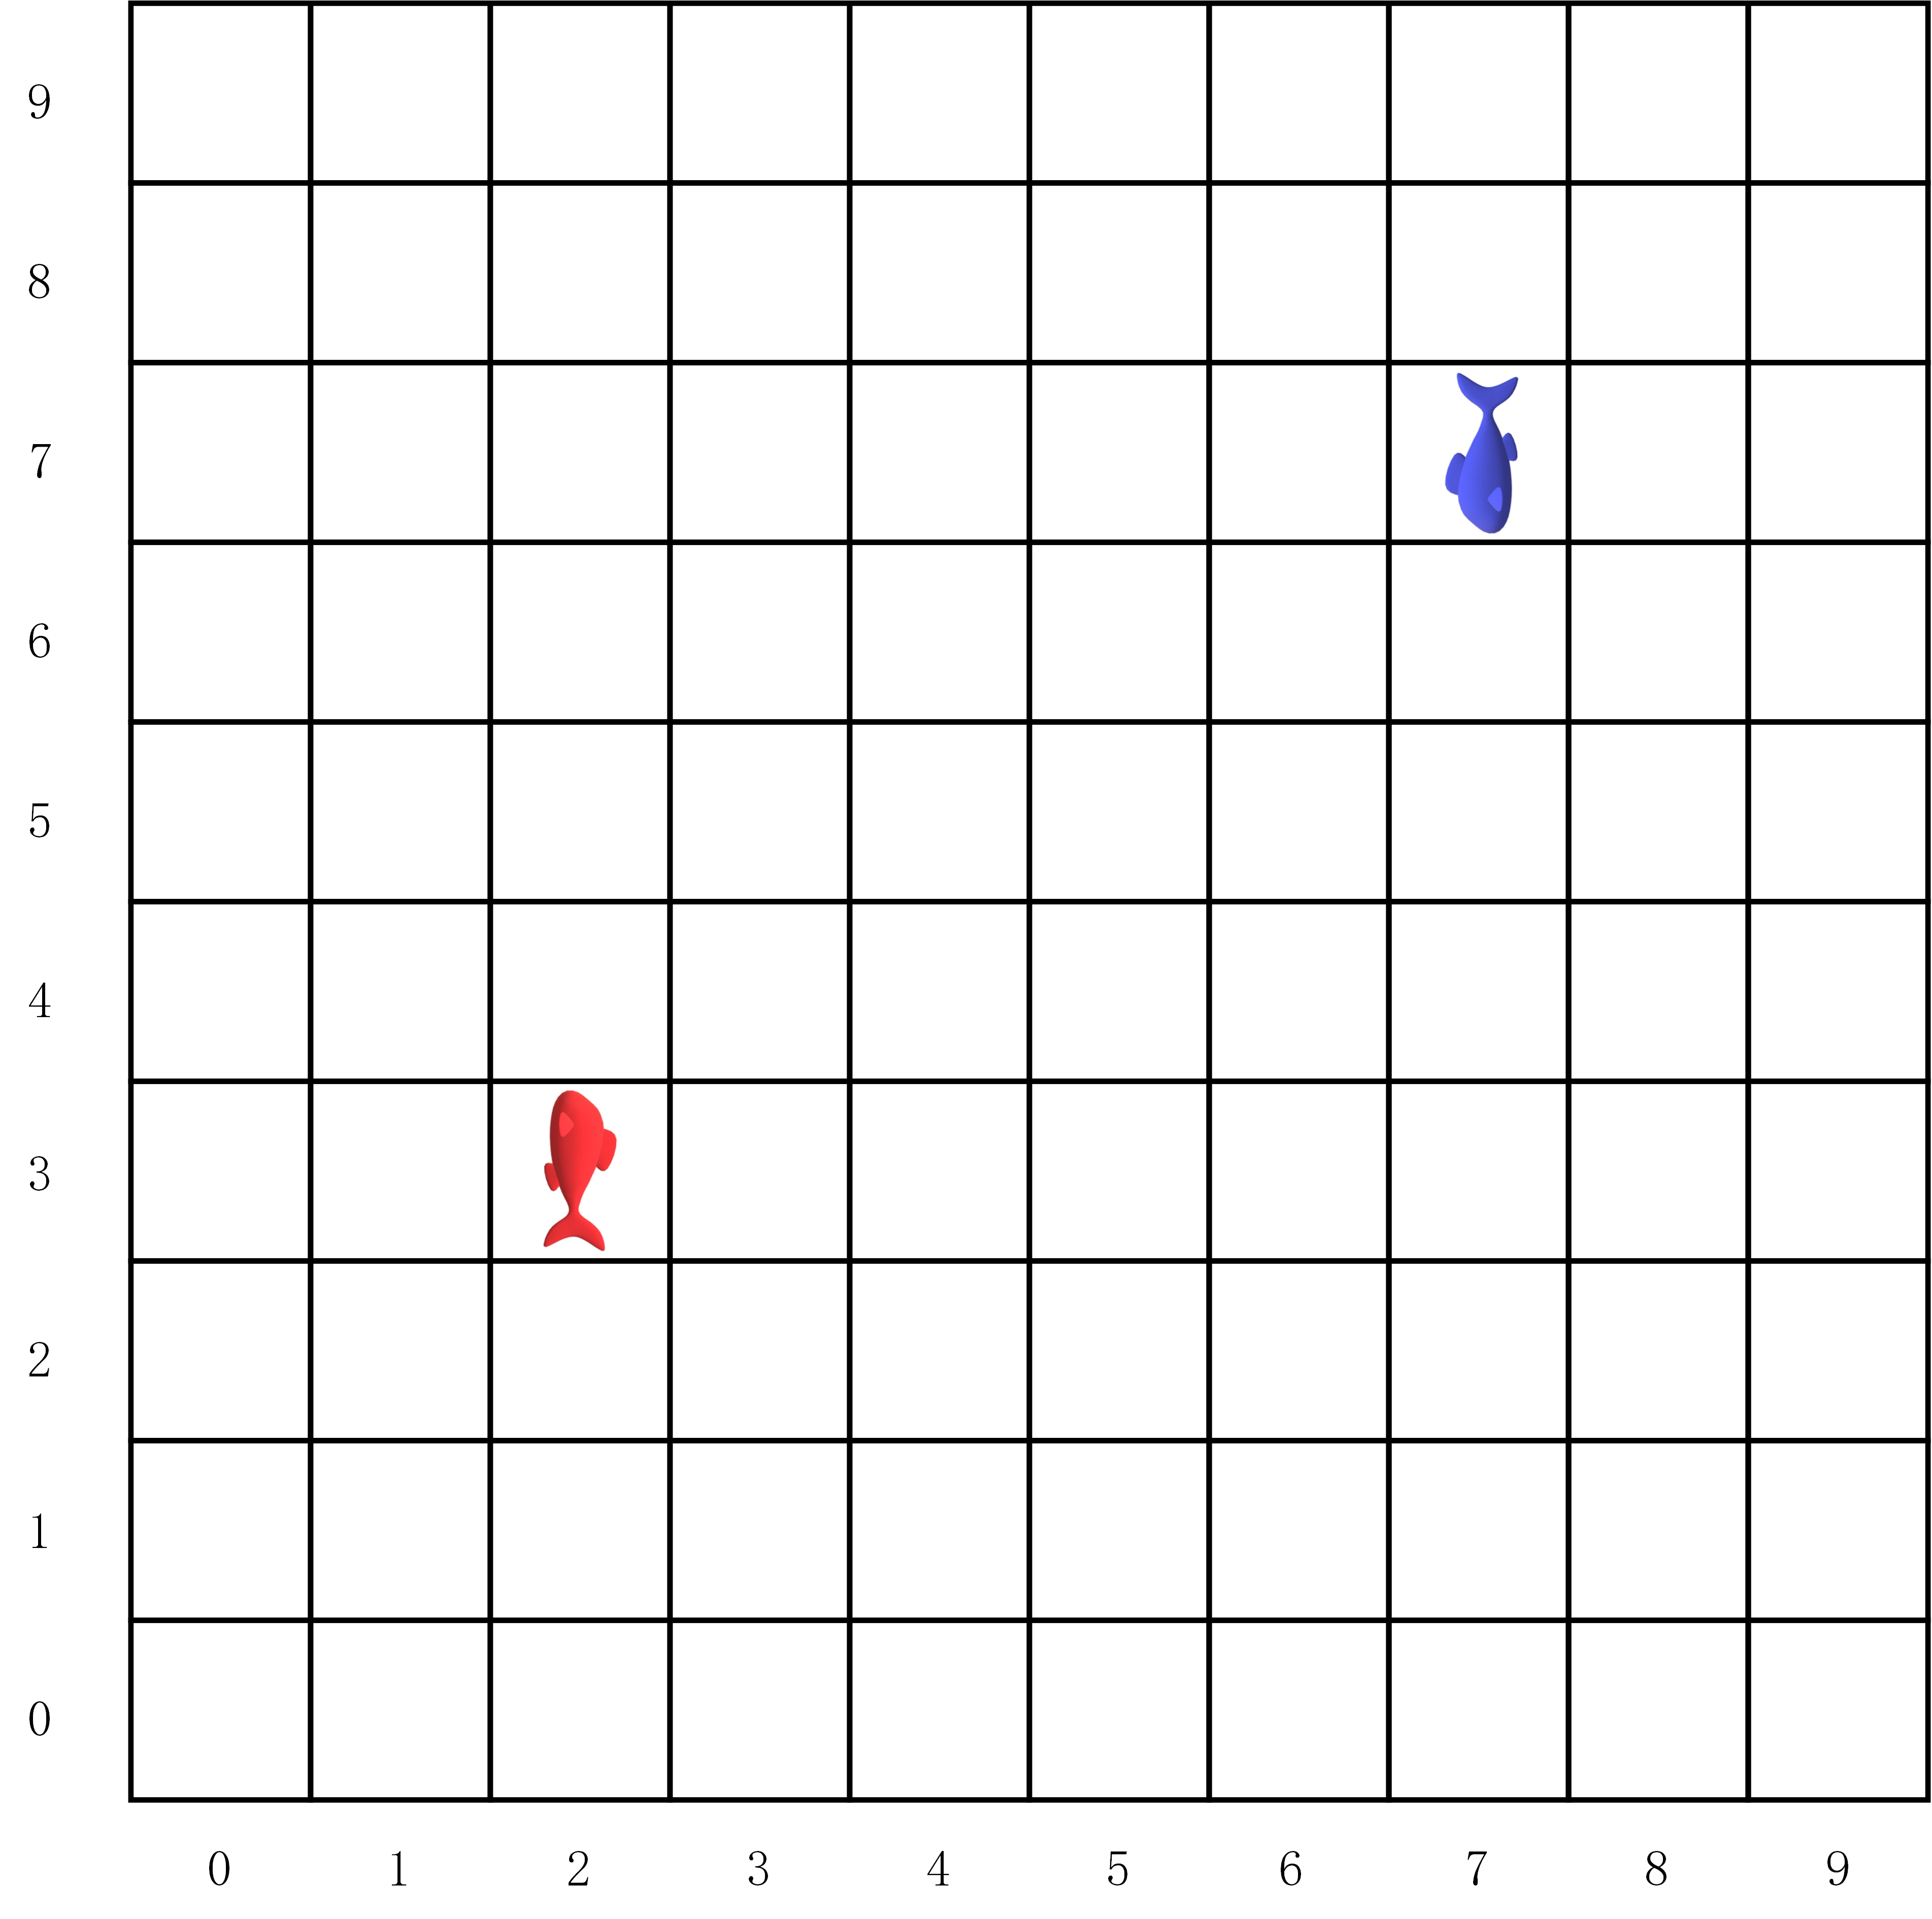
\includegraphics[width=10cm]{example/yiduiyi1.jpg}
	\bicaption[这里将出现在插图索引]
	{红蓝两方初始状态}
	{Neural network training pipeline}
	\label{yiduiyi1.jpg}
\end{figure}
红方为先行玩家,首先让红方向右走一步,得到蓝方的动作概率,如图\ref{yiduiyi2.jpg}


\begin{figure}[!hbtp]
	\centering
	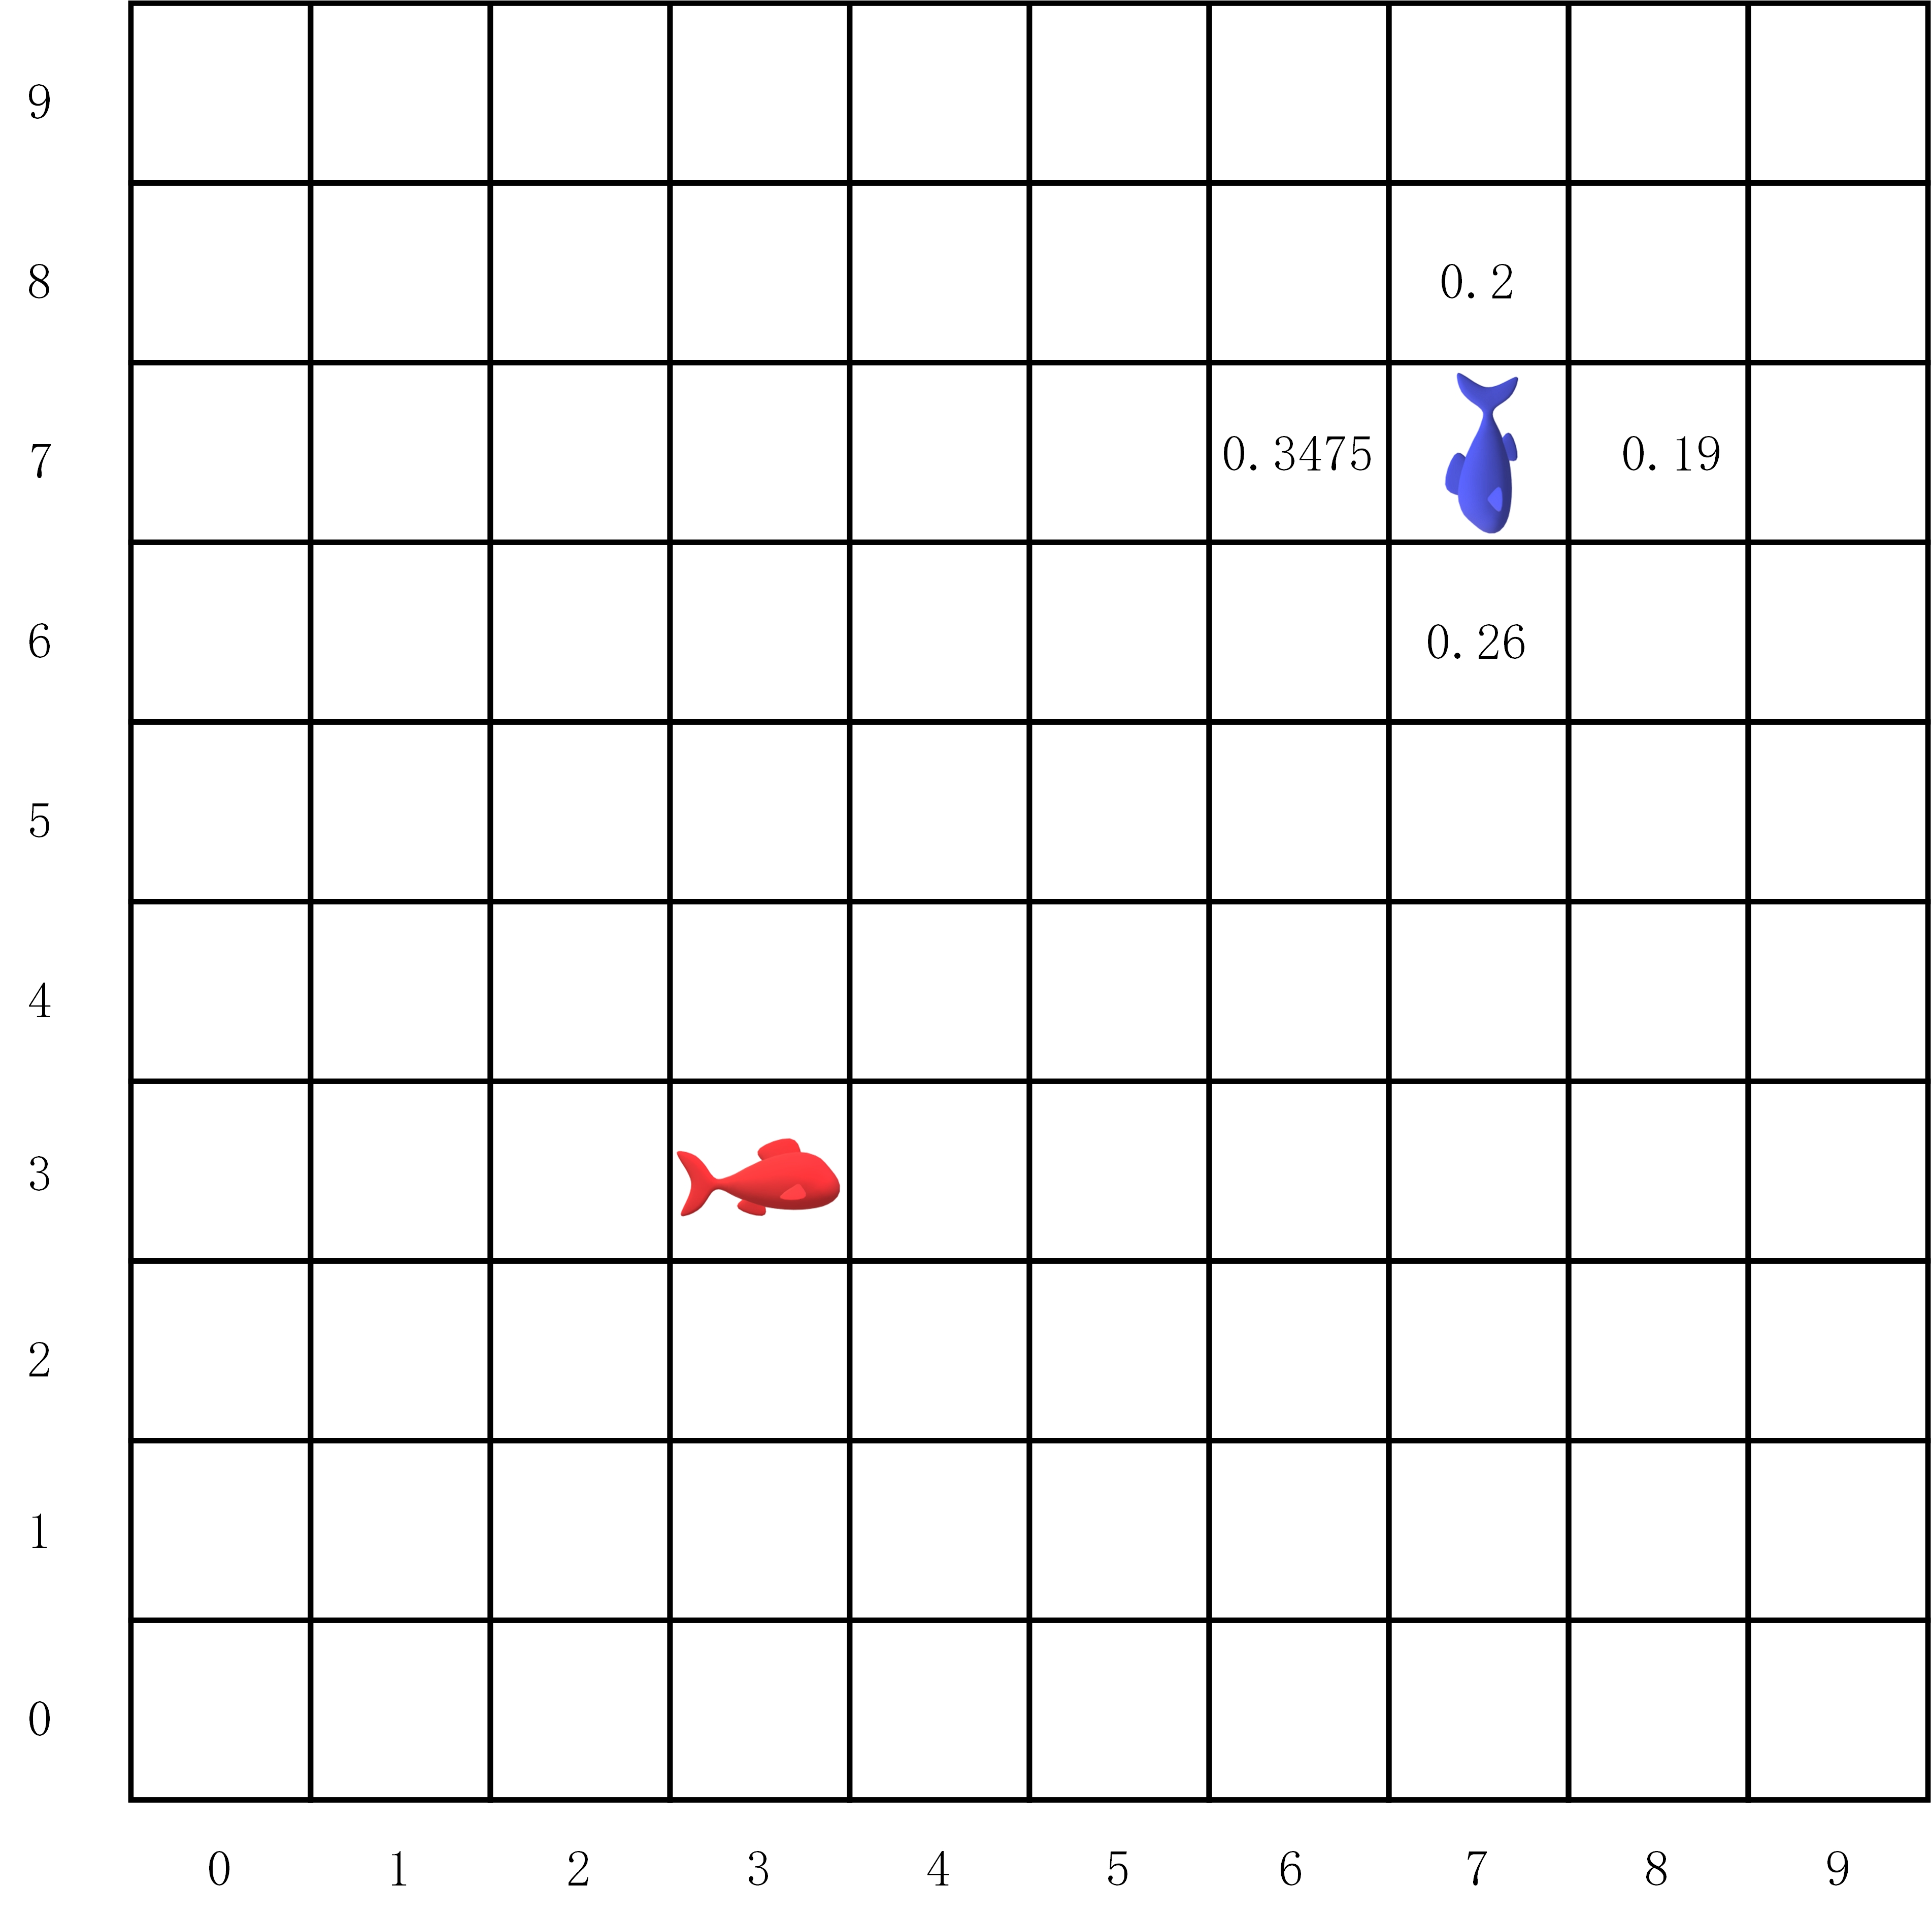
\includegraphics[width=10cm]{example/yiduiyi2.jpg}
	\bicaption[这里将出现在插图索引]
	{红蓝两方初始状态}
	{Neural network training pipeline}
	\label{yiduiyi2.jpg}
\end{figure}

接着蓝方取动作概率中的最大值进行动作,人机对弈的结果如下:


\begin{figure}[!htp]
	\centering
	\subcaptionbox{\label{fig2:yiduiyi3-6:a}}
	{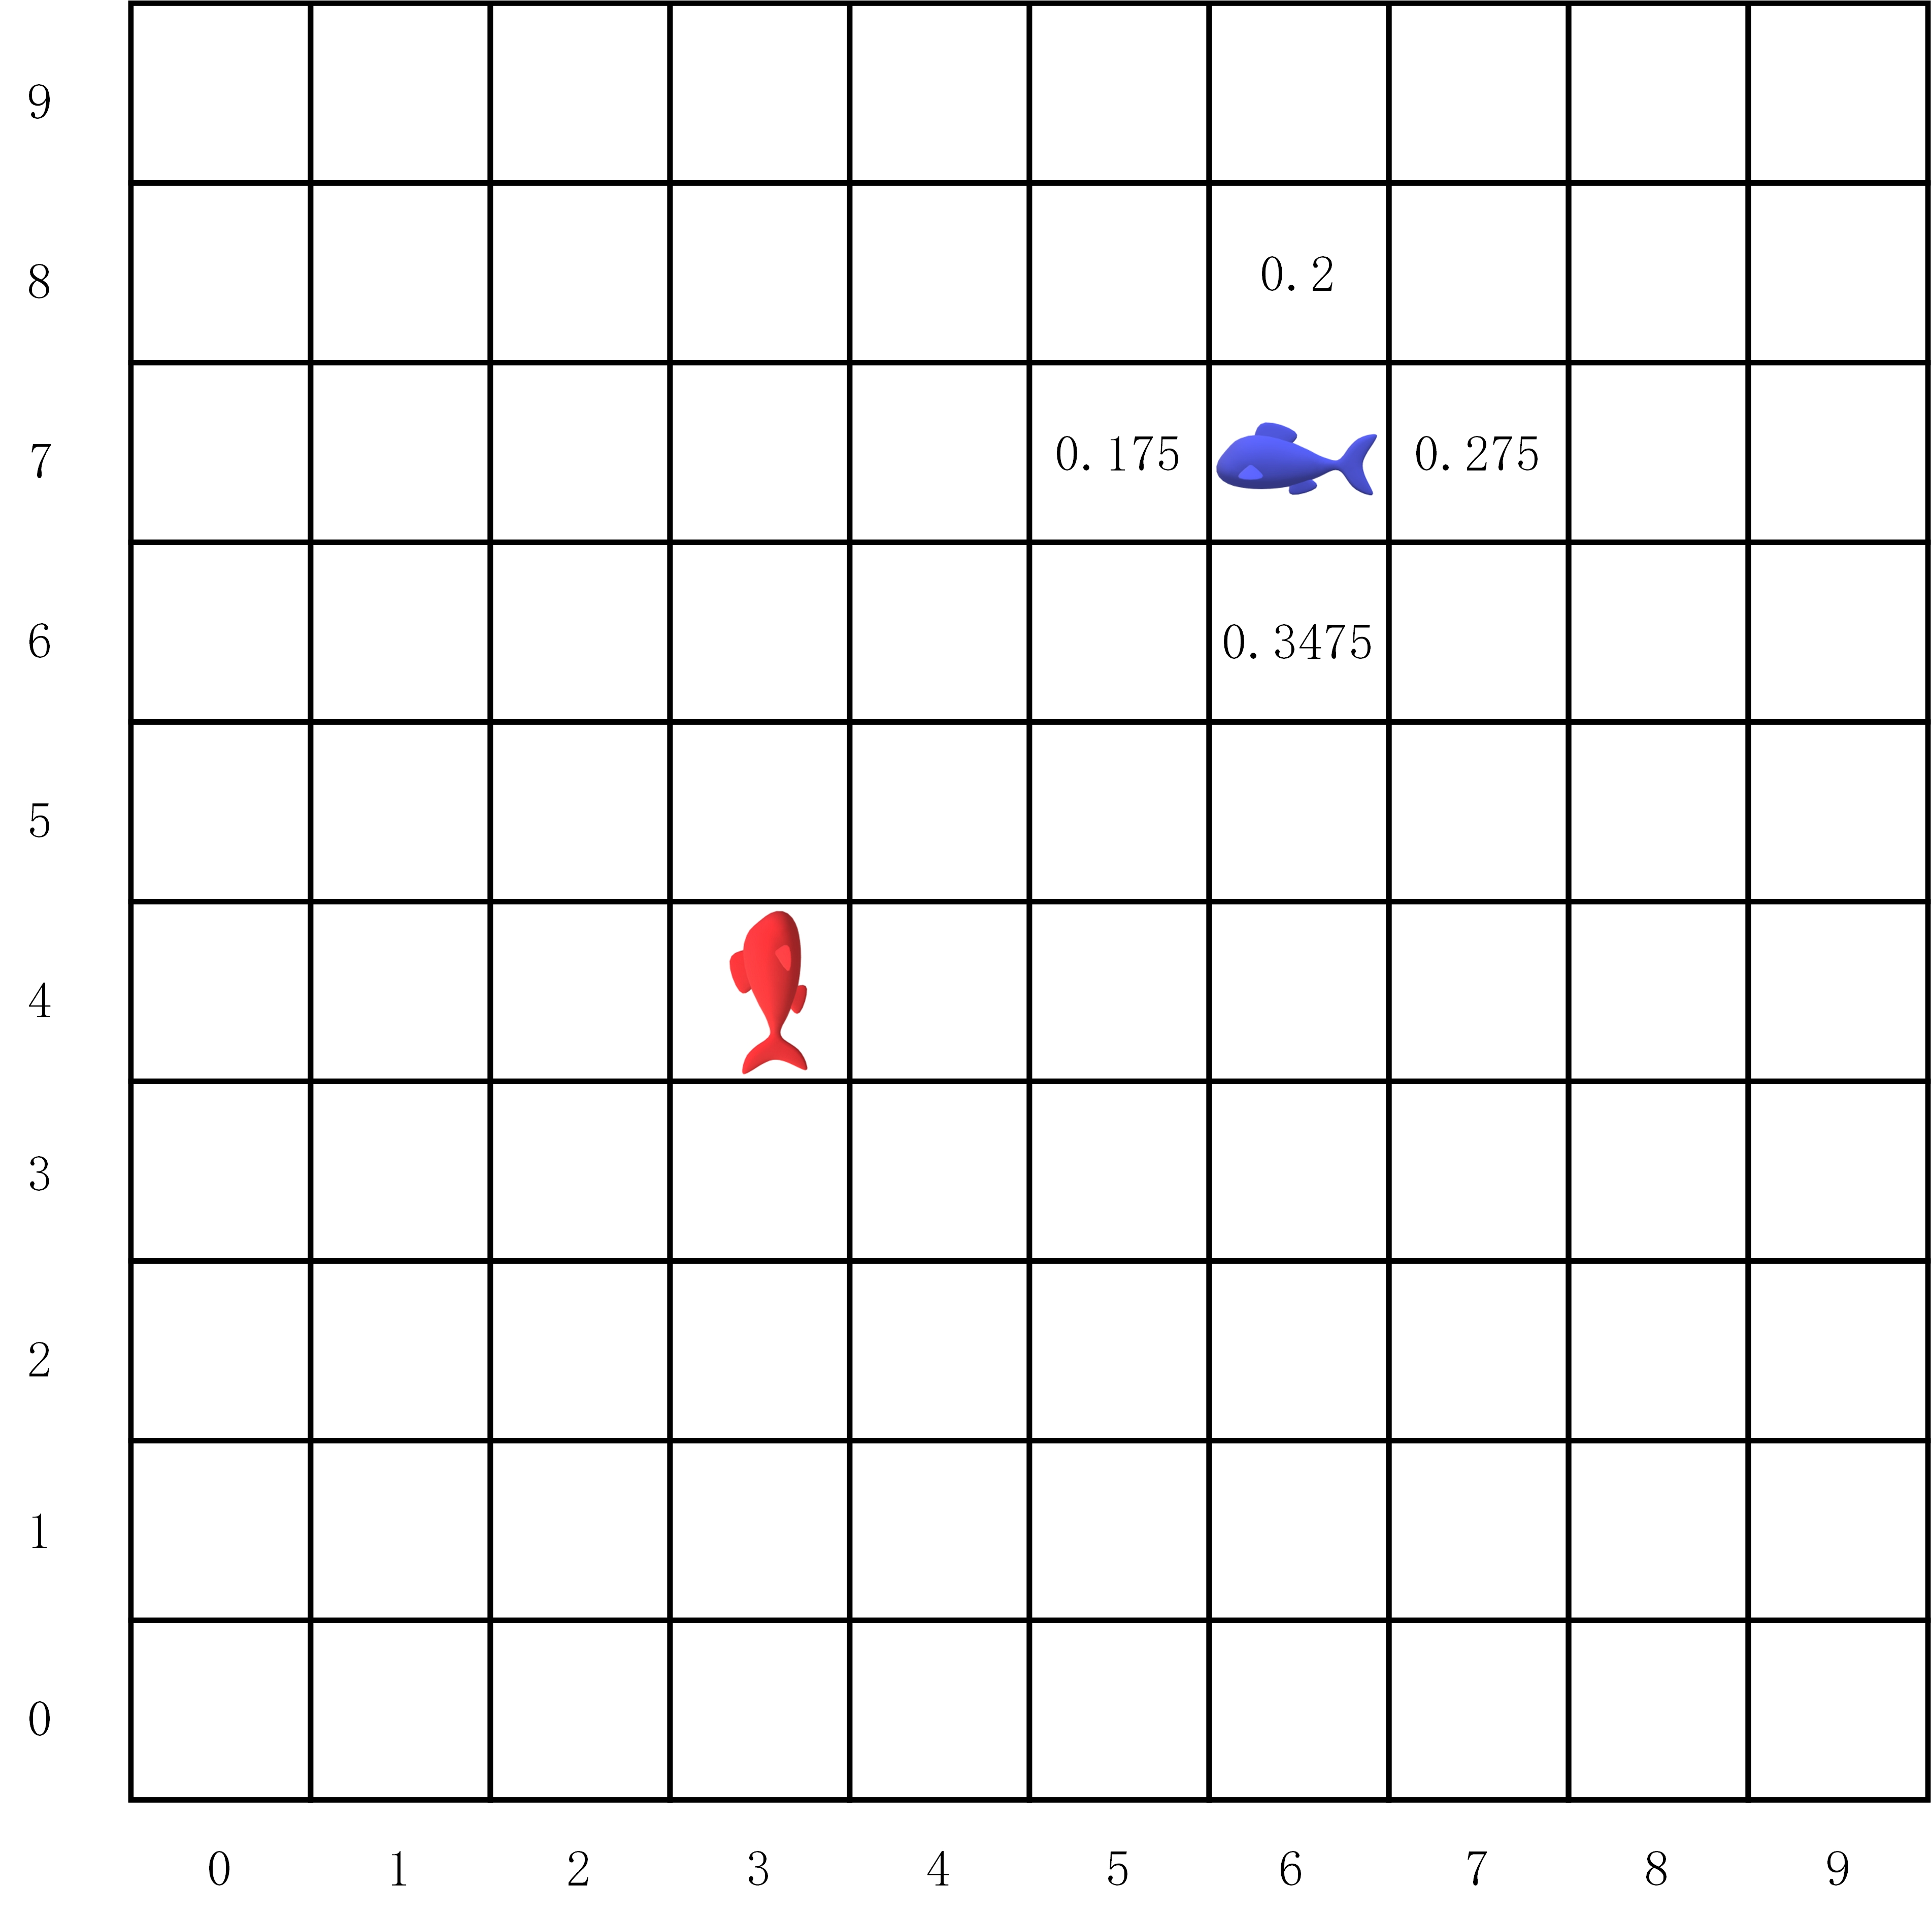
\includegraphics[width=0.45\hsize,height=0.45\hsize]{example/yiduiyi3.jpg}}
	\hspace{0.5em}
	\subcaptionbox{\label{fig2:yiduiyi3-6:b}}
	{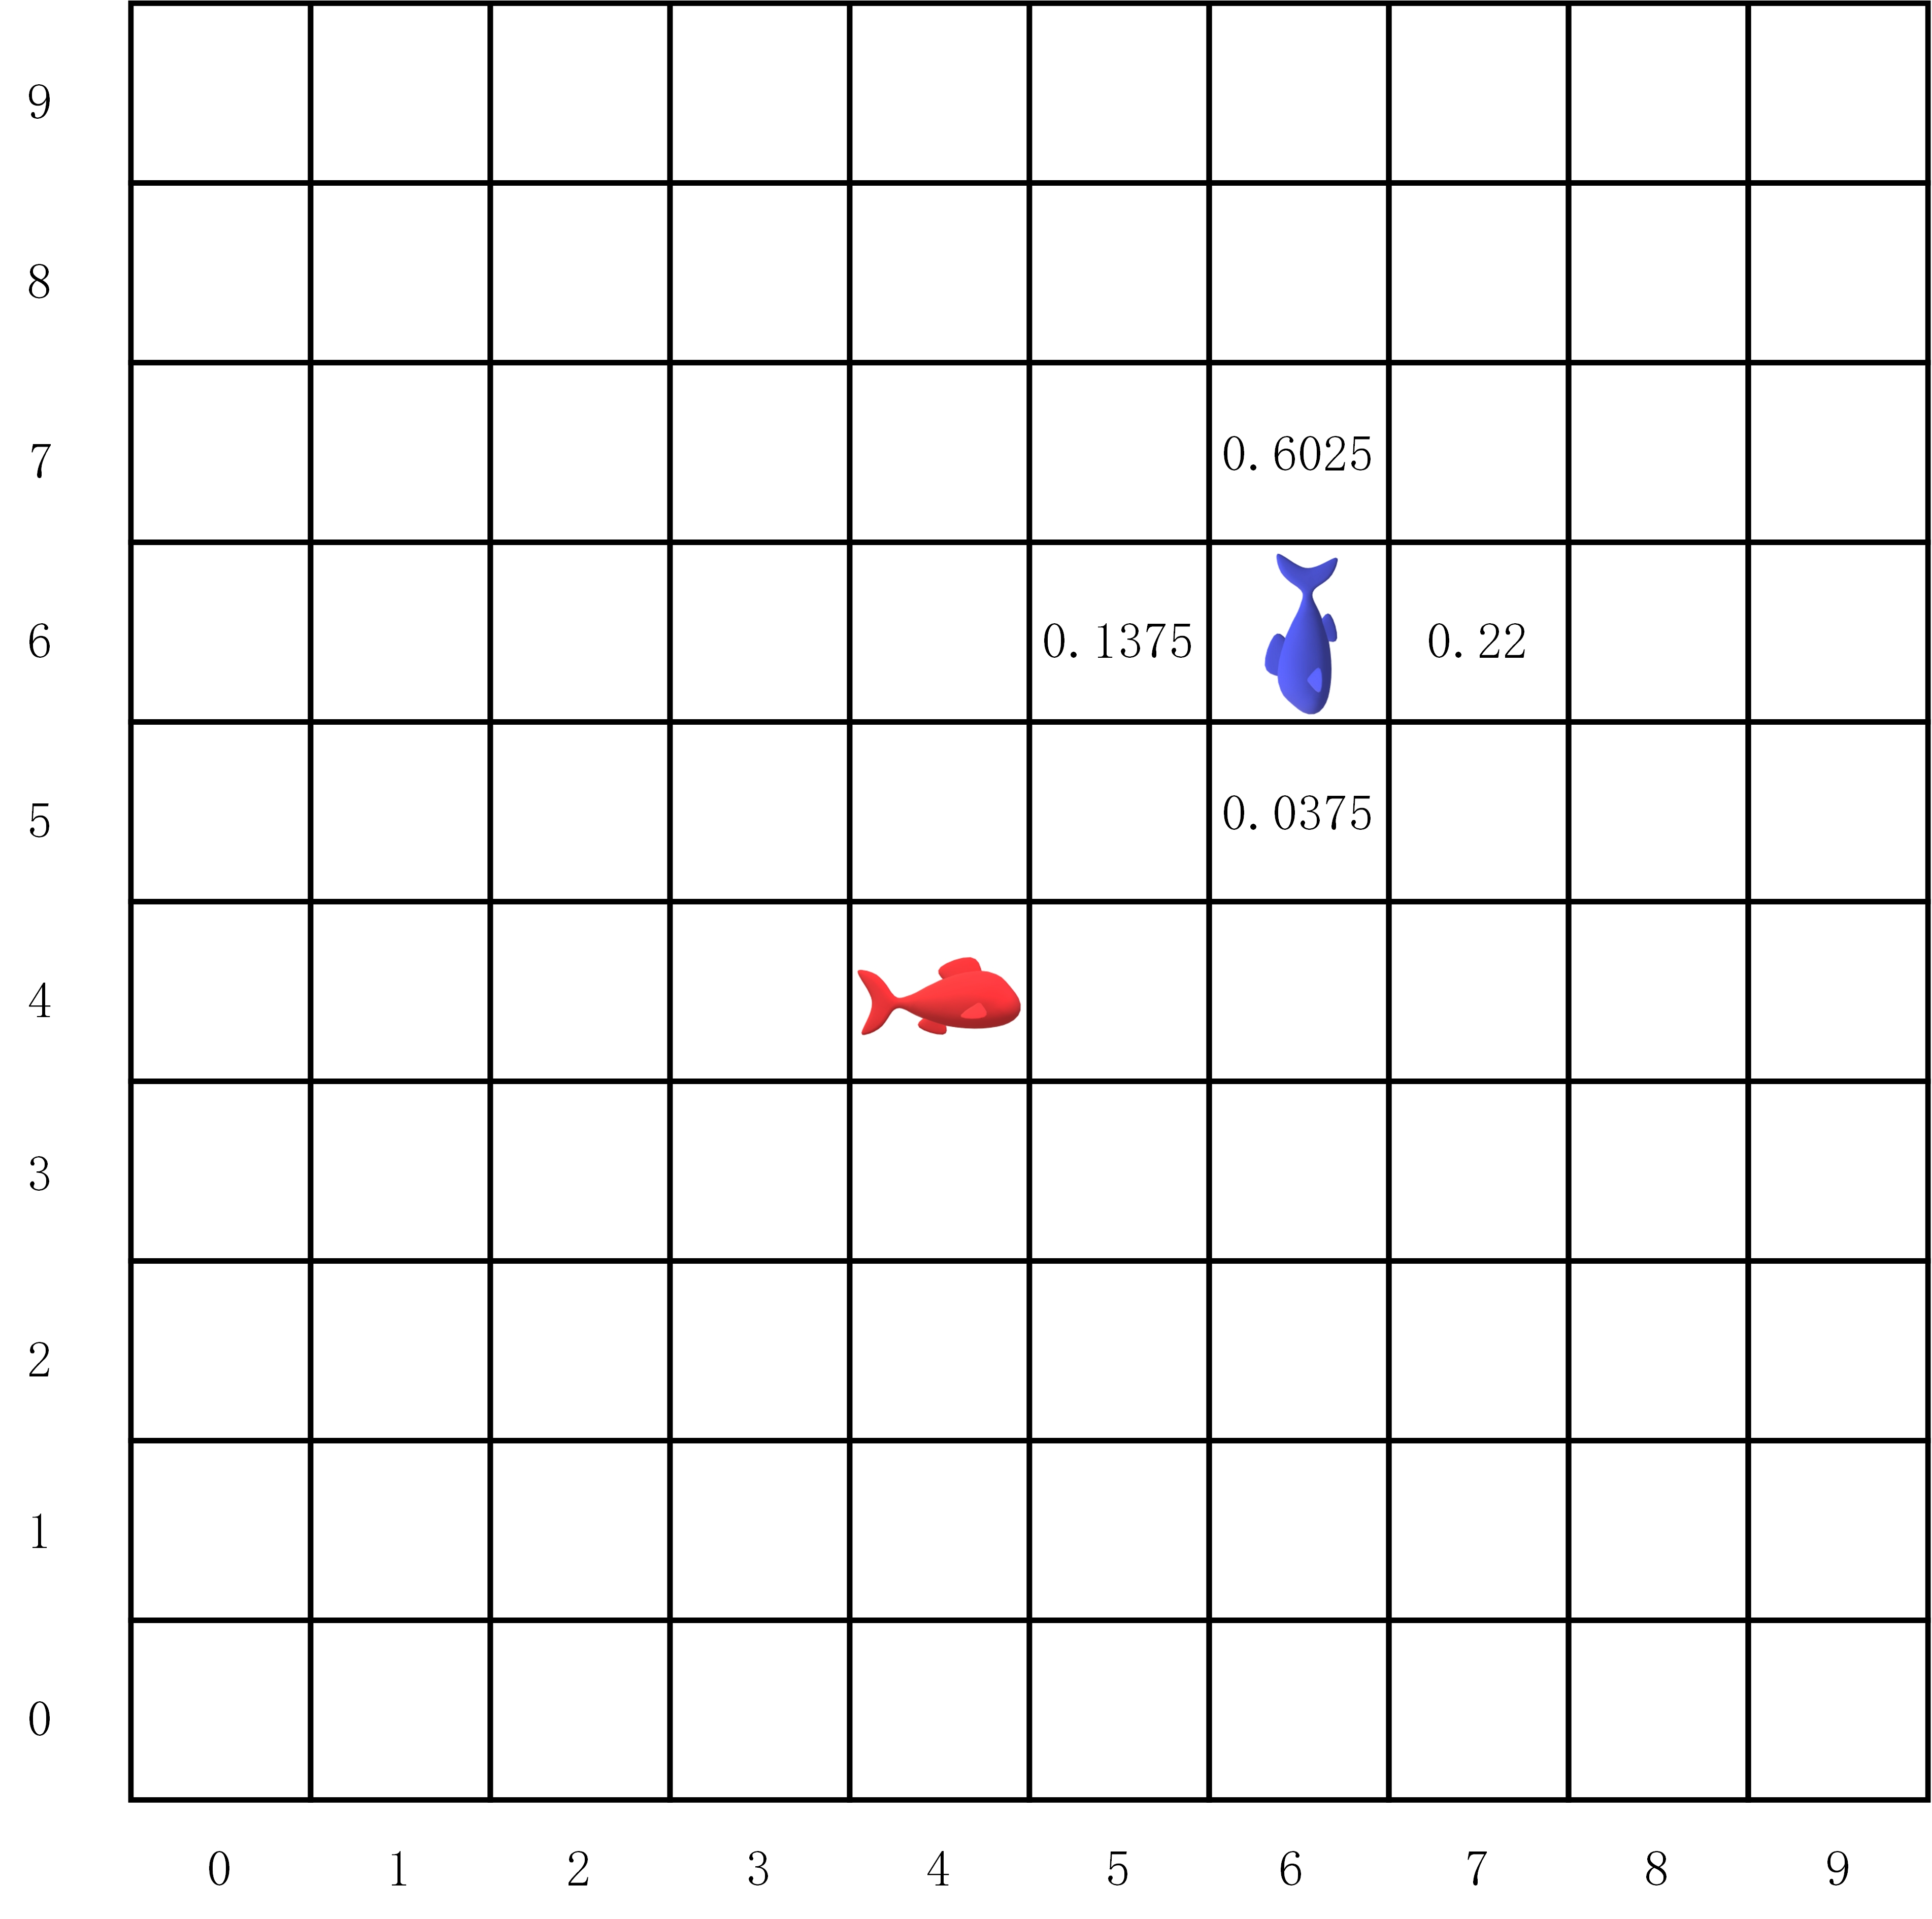
\includegraphics[width=0.45\hsize,height=0.45\hsize]{example/yiduiyi4.jpg}}
	\newline
	\centering
	\subcaptionbox{\label{fig2:yiduiyi3-6:c}}
	{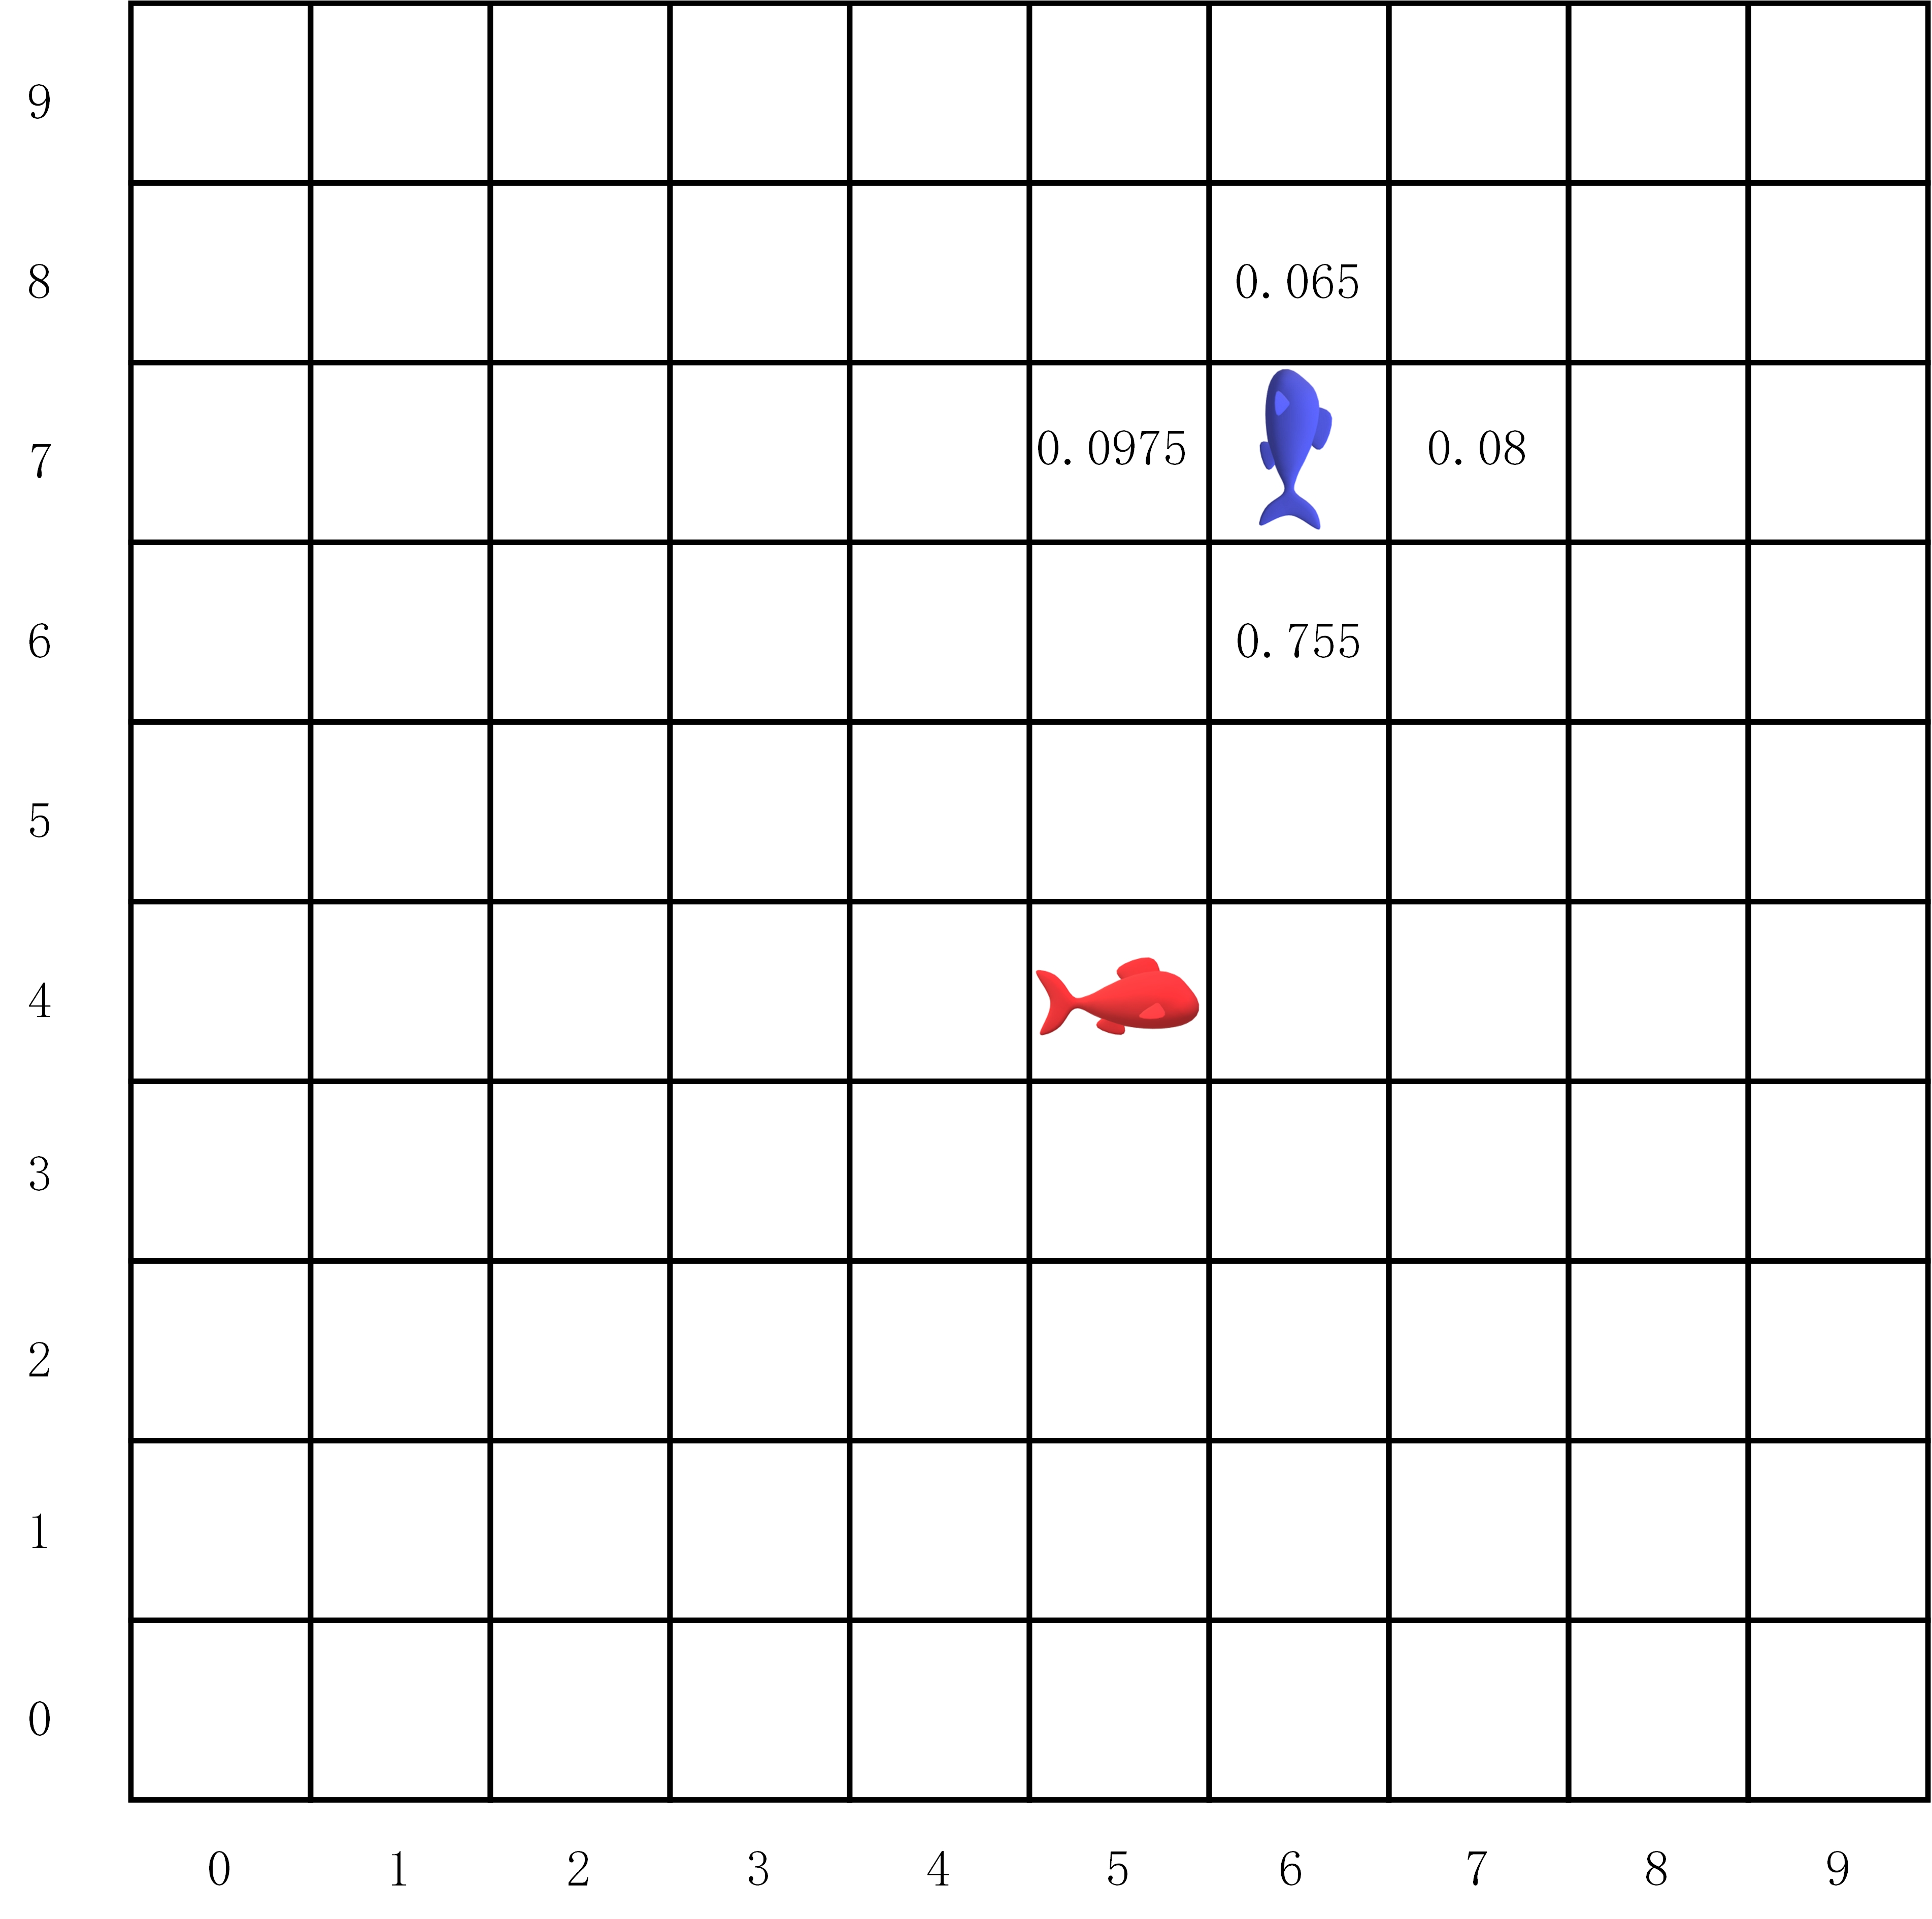
\includegraphics[width=0.45\hsize,height=0.45\hsize]{example/yiduiyi5.jpg}}
	\hspace{0.5em}
	\subcaptionbox{\label{fig2:yiduiyi3-6:d}}
	{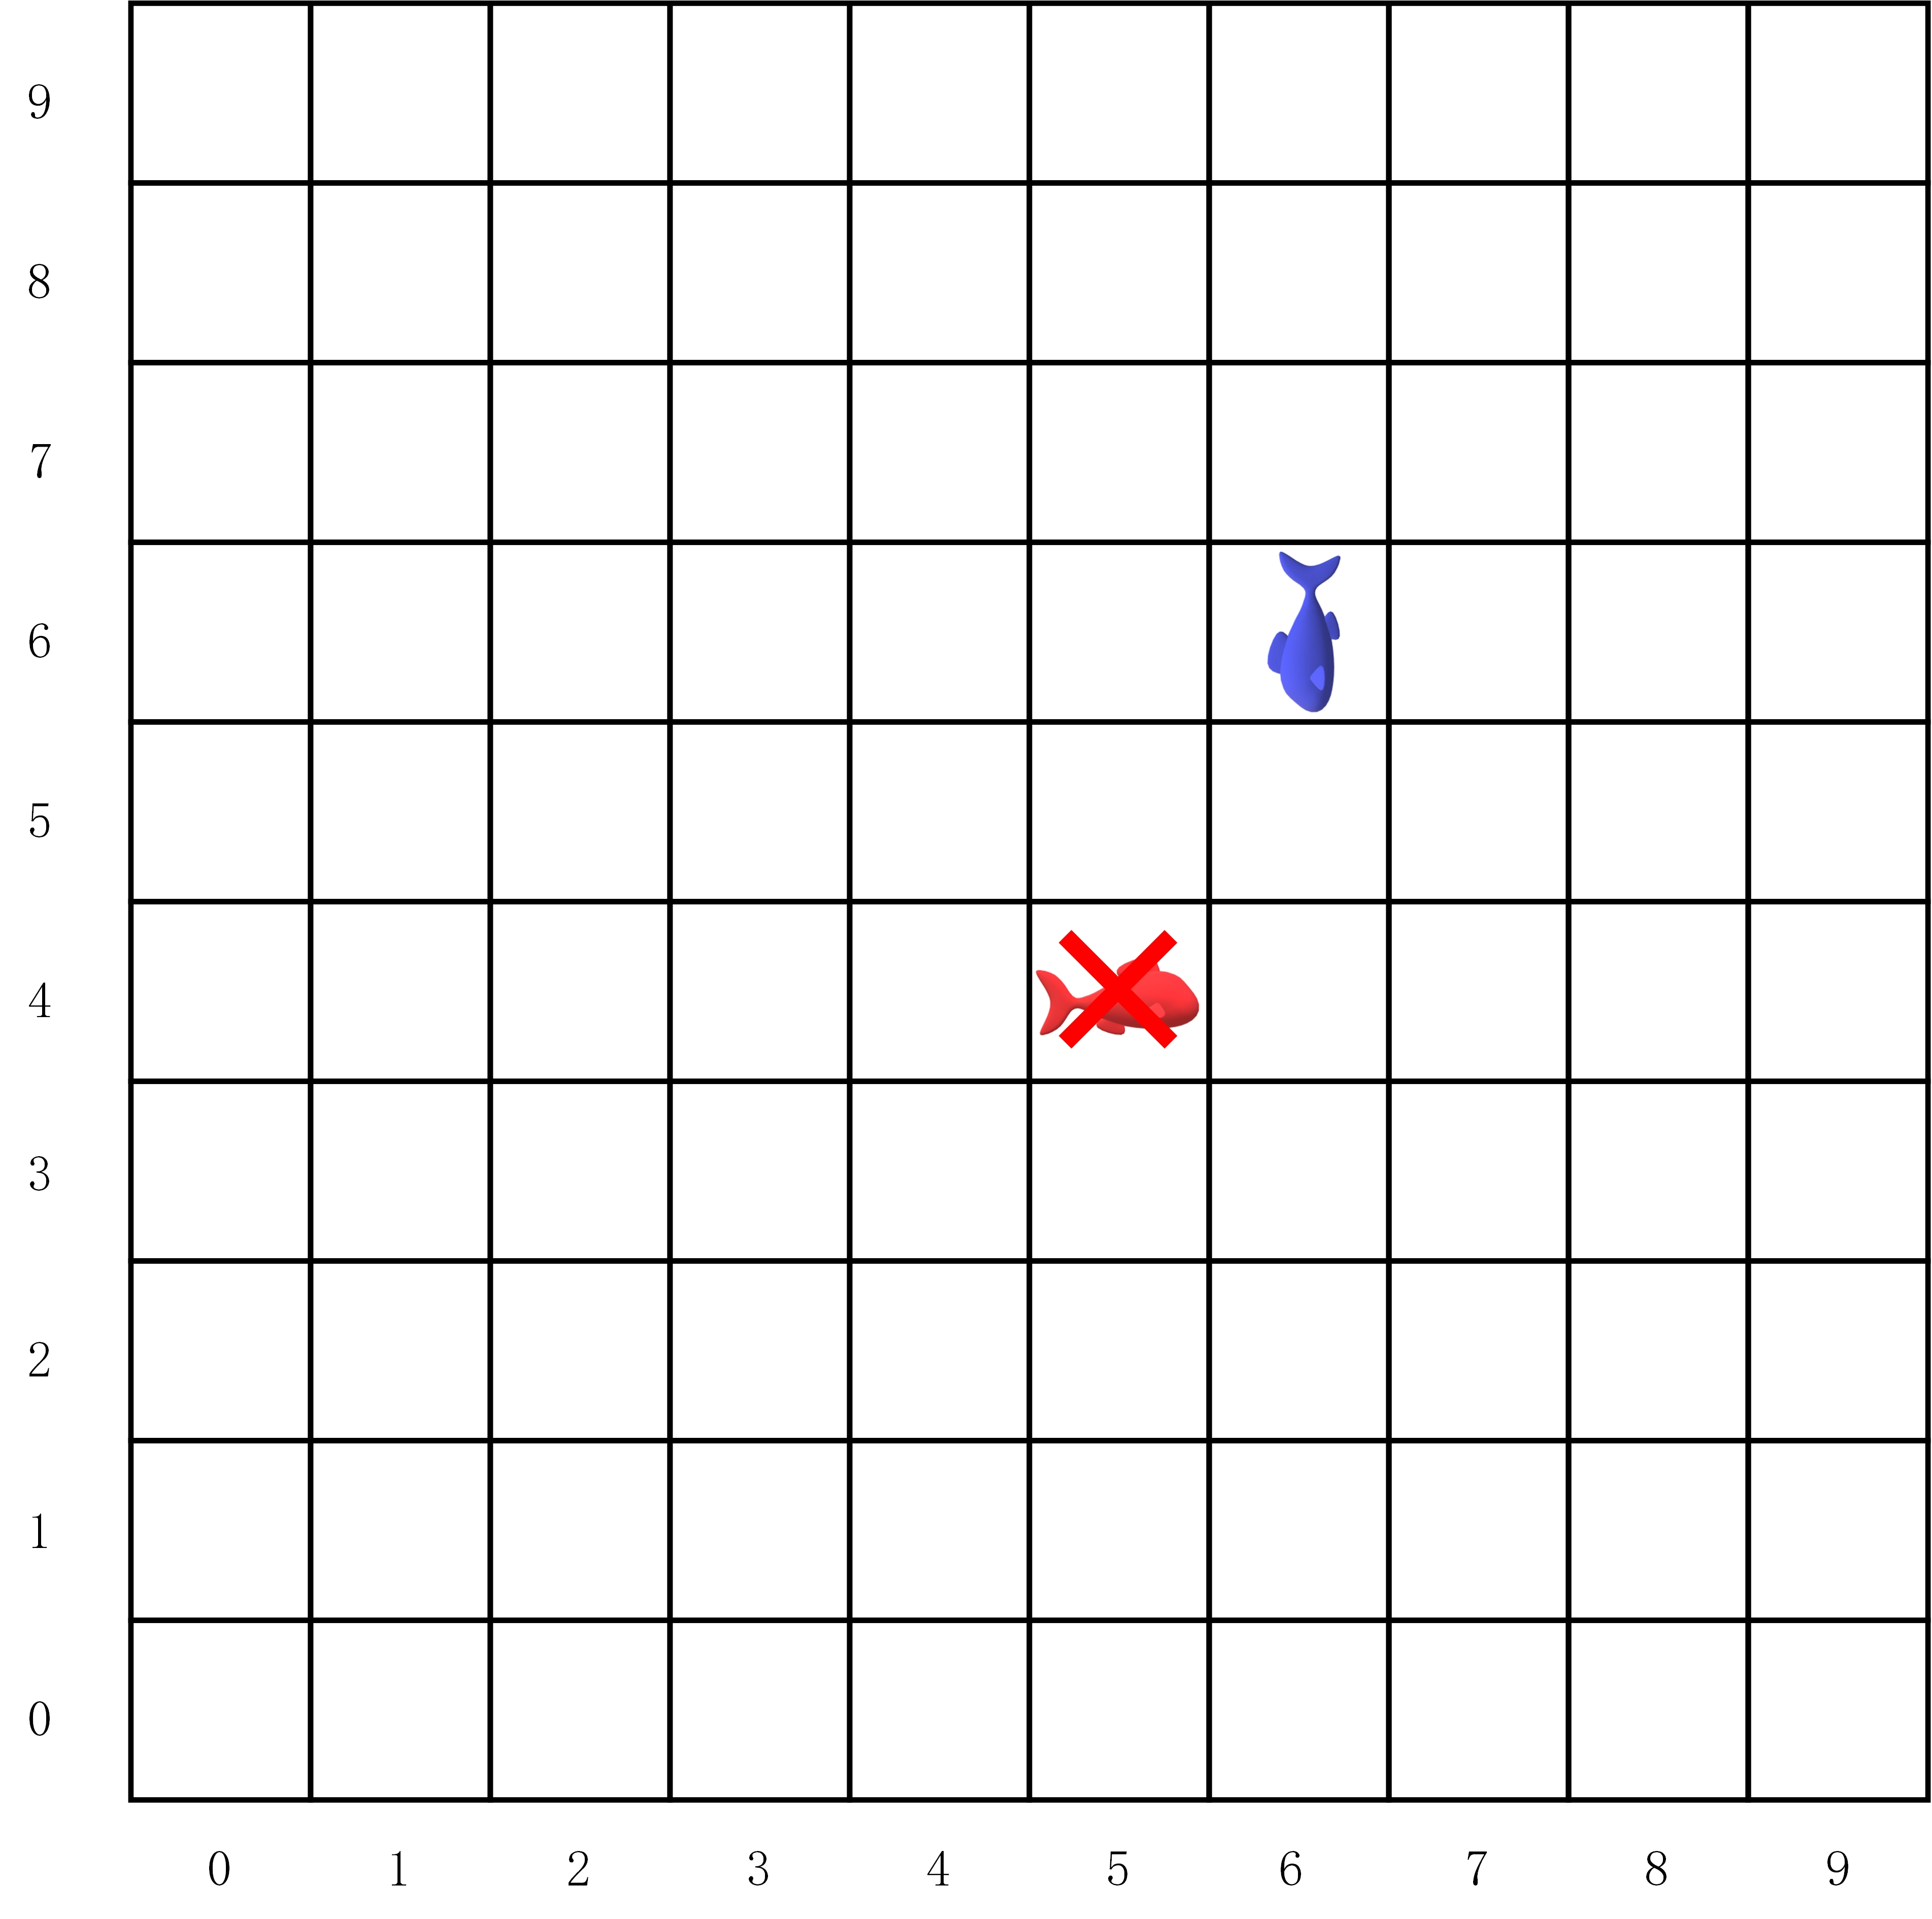
\includegraphics[width=0.45\hsize,height=0.45\hsize]{example/yiduiyi6.jpg}}
	\bicaption
	{一对一人机对弈过程图示}
	{Examples of response maps during occlusions and not.The first row shows the original and response maps with no occlusions while the second row shows the maps with occlusions. The first column are the shots of sequence bear front in Princeton dataset. The color response maps are in the second column while the depth’s are in the third.}
	\label{fig2:yiduiyi3-6}
\end{figure}

对于\ref{fig2:yiduiyi3-6:b}状态,假设蓝方分别执行四个动作,看其和红方的相对状态:
\begin{figure}[!htp]
	\centering
	\subcaptionbox{向上双方状态\label{fig2:yiduiyi7-10:a}}
	{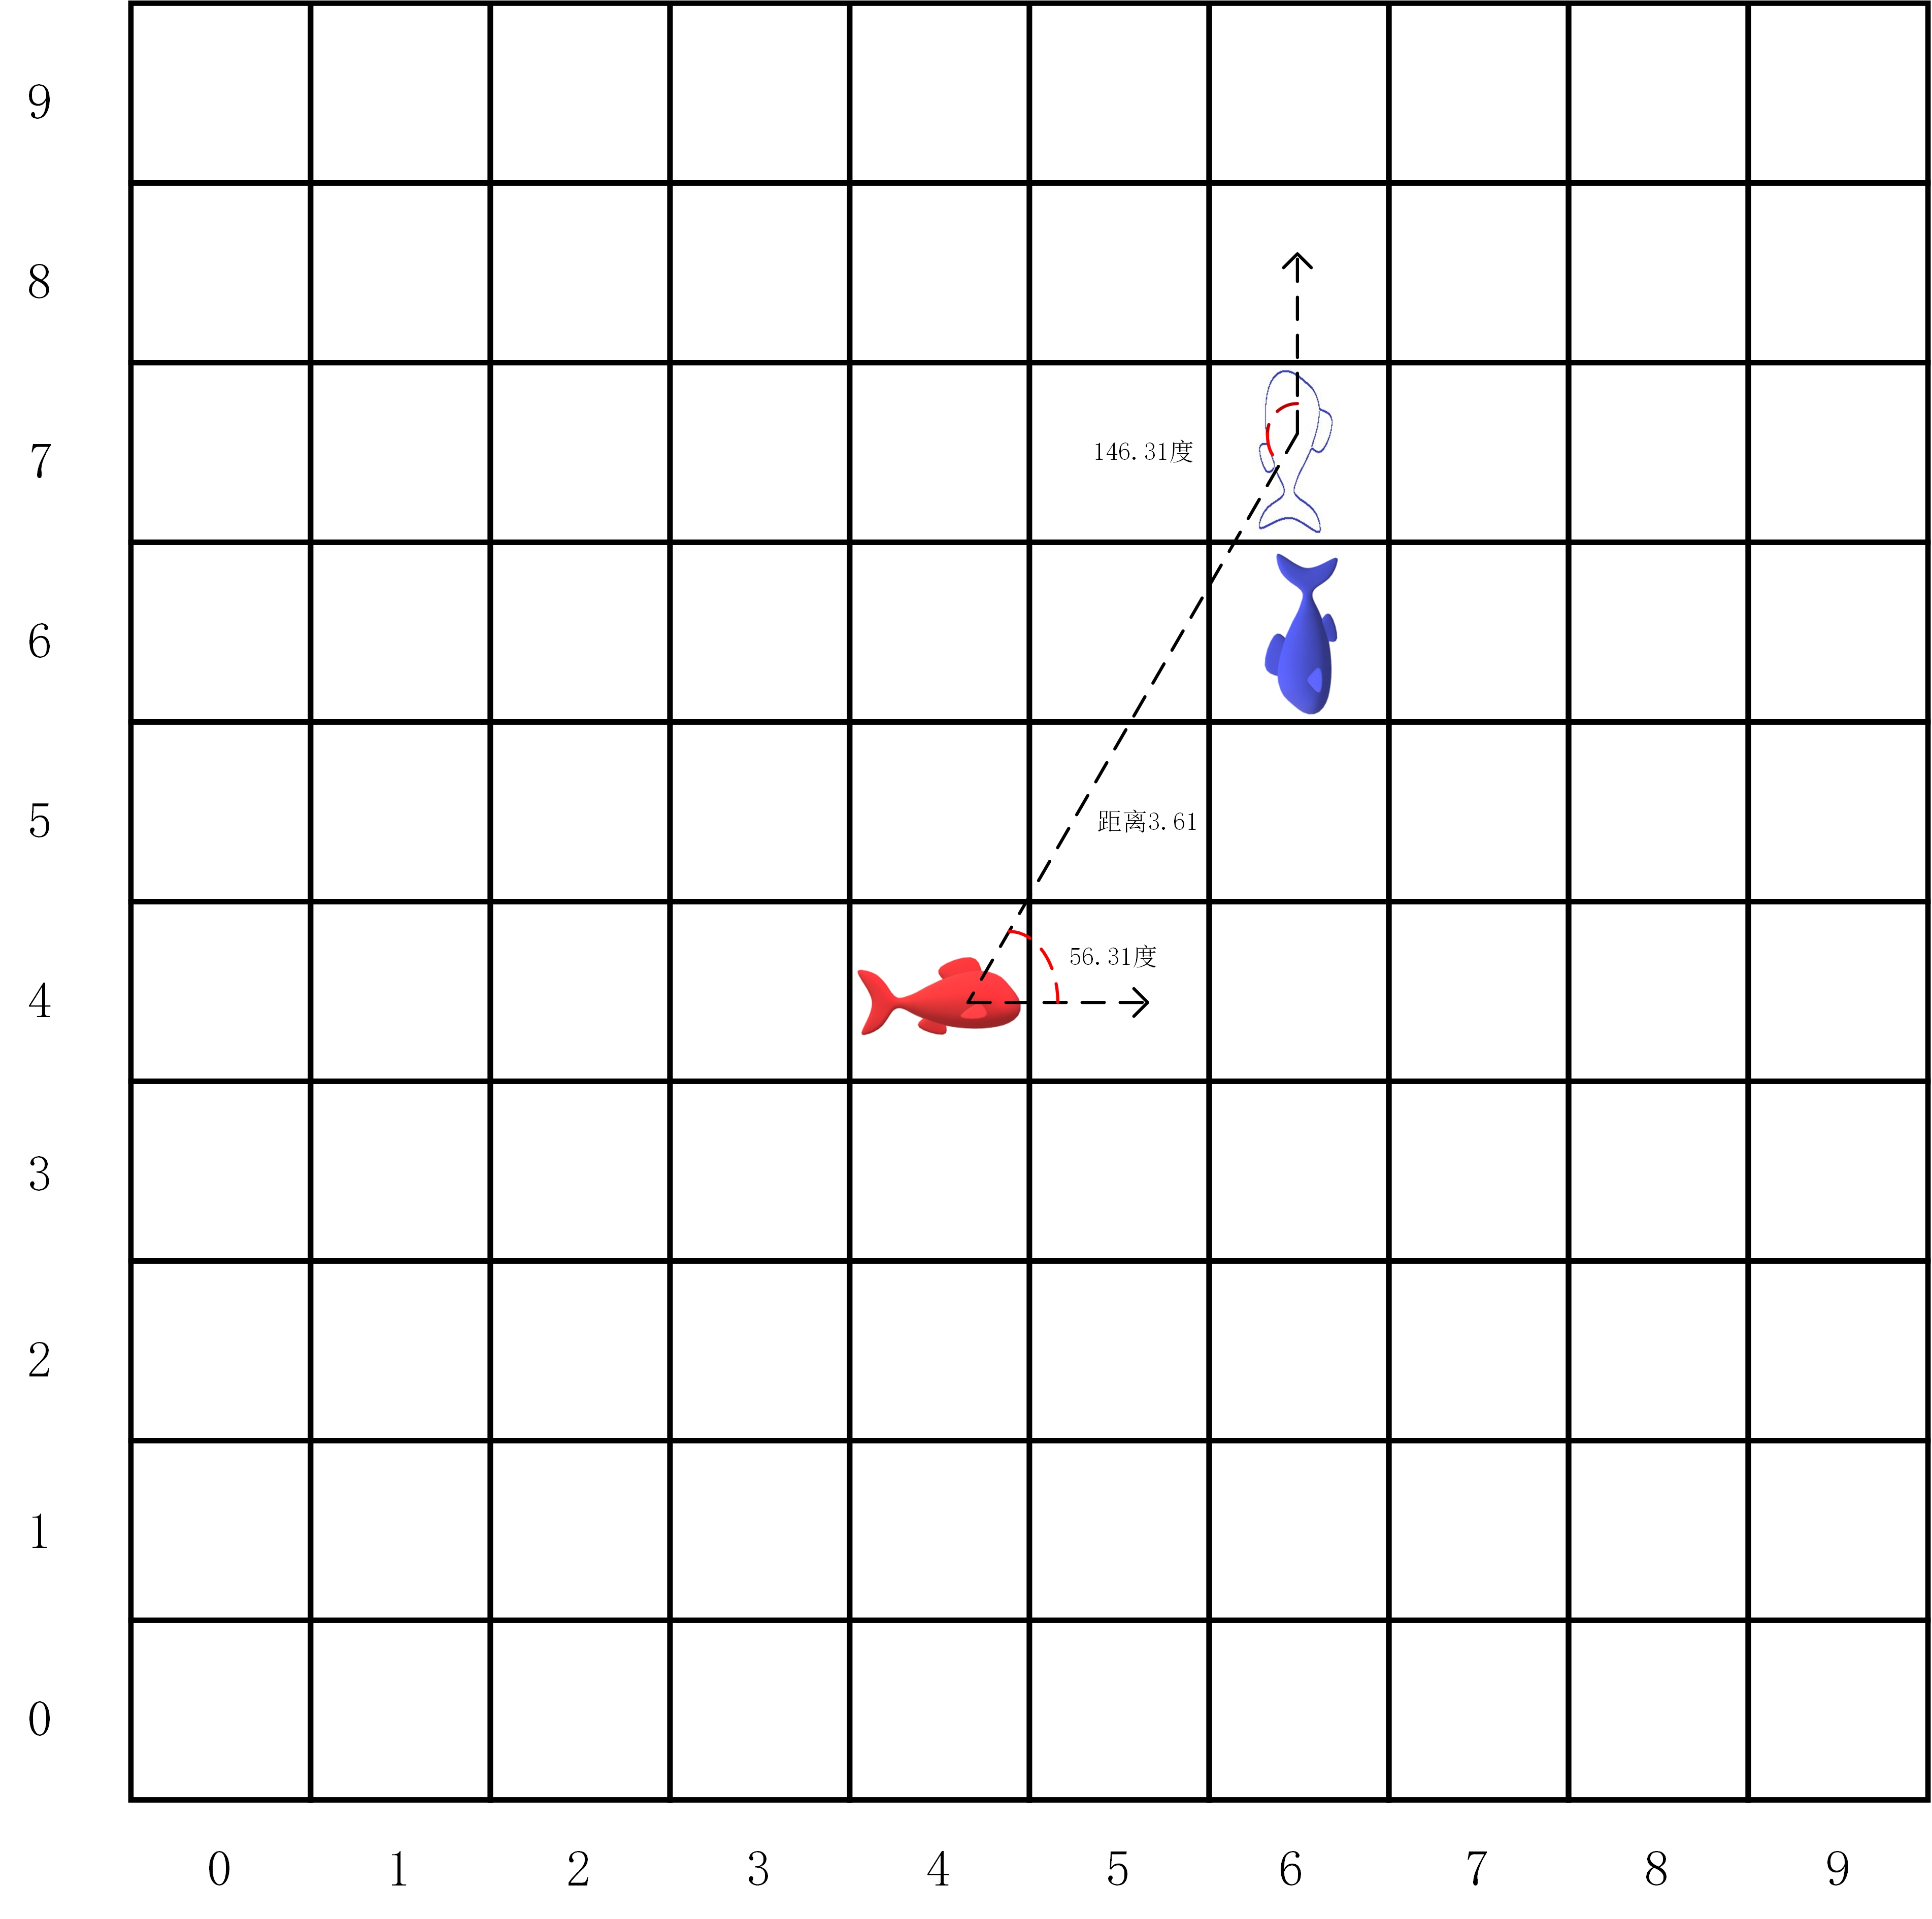
\includegraphics[width=0.45\hsize,height=0.45\hsize]{example/yiduiyi7.jpg}}
	\hspace{0.5em}
	\subcaptionbox{向下双方状态\label{fig2:yiduiyi7-10:b}}
	{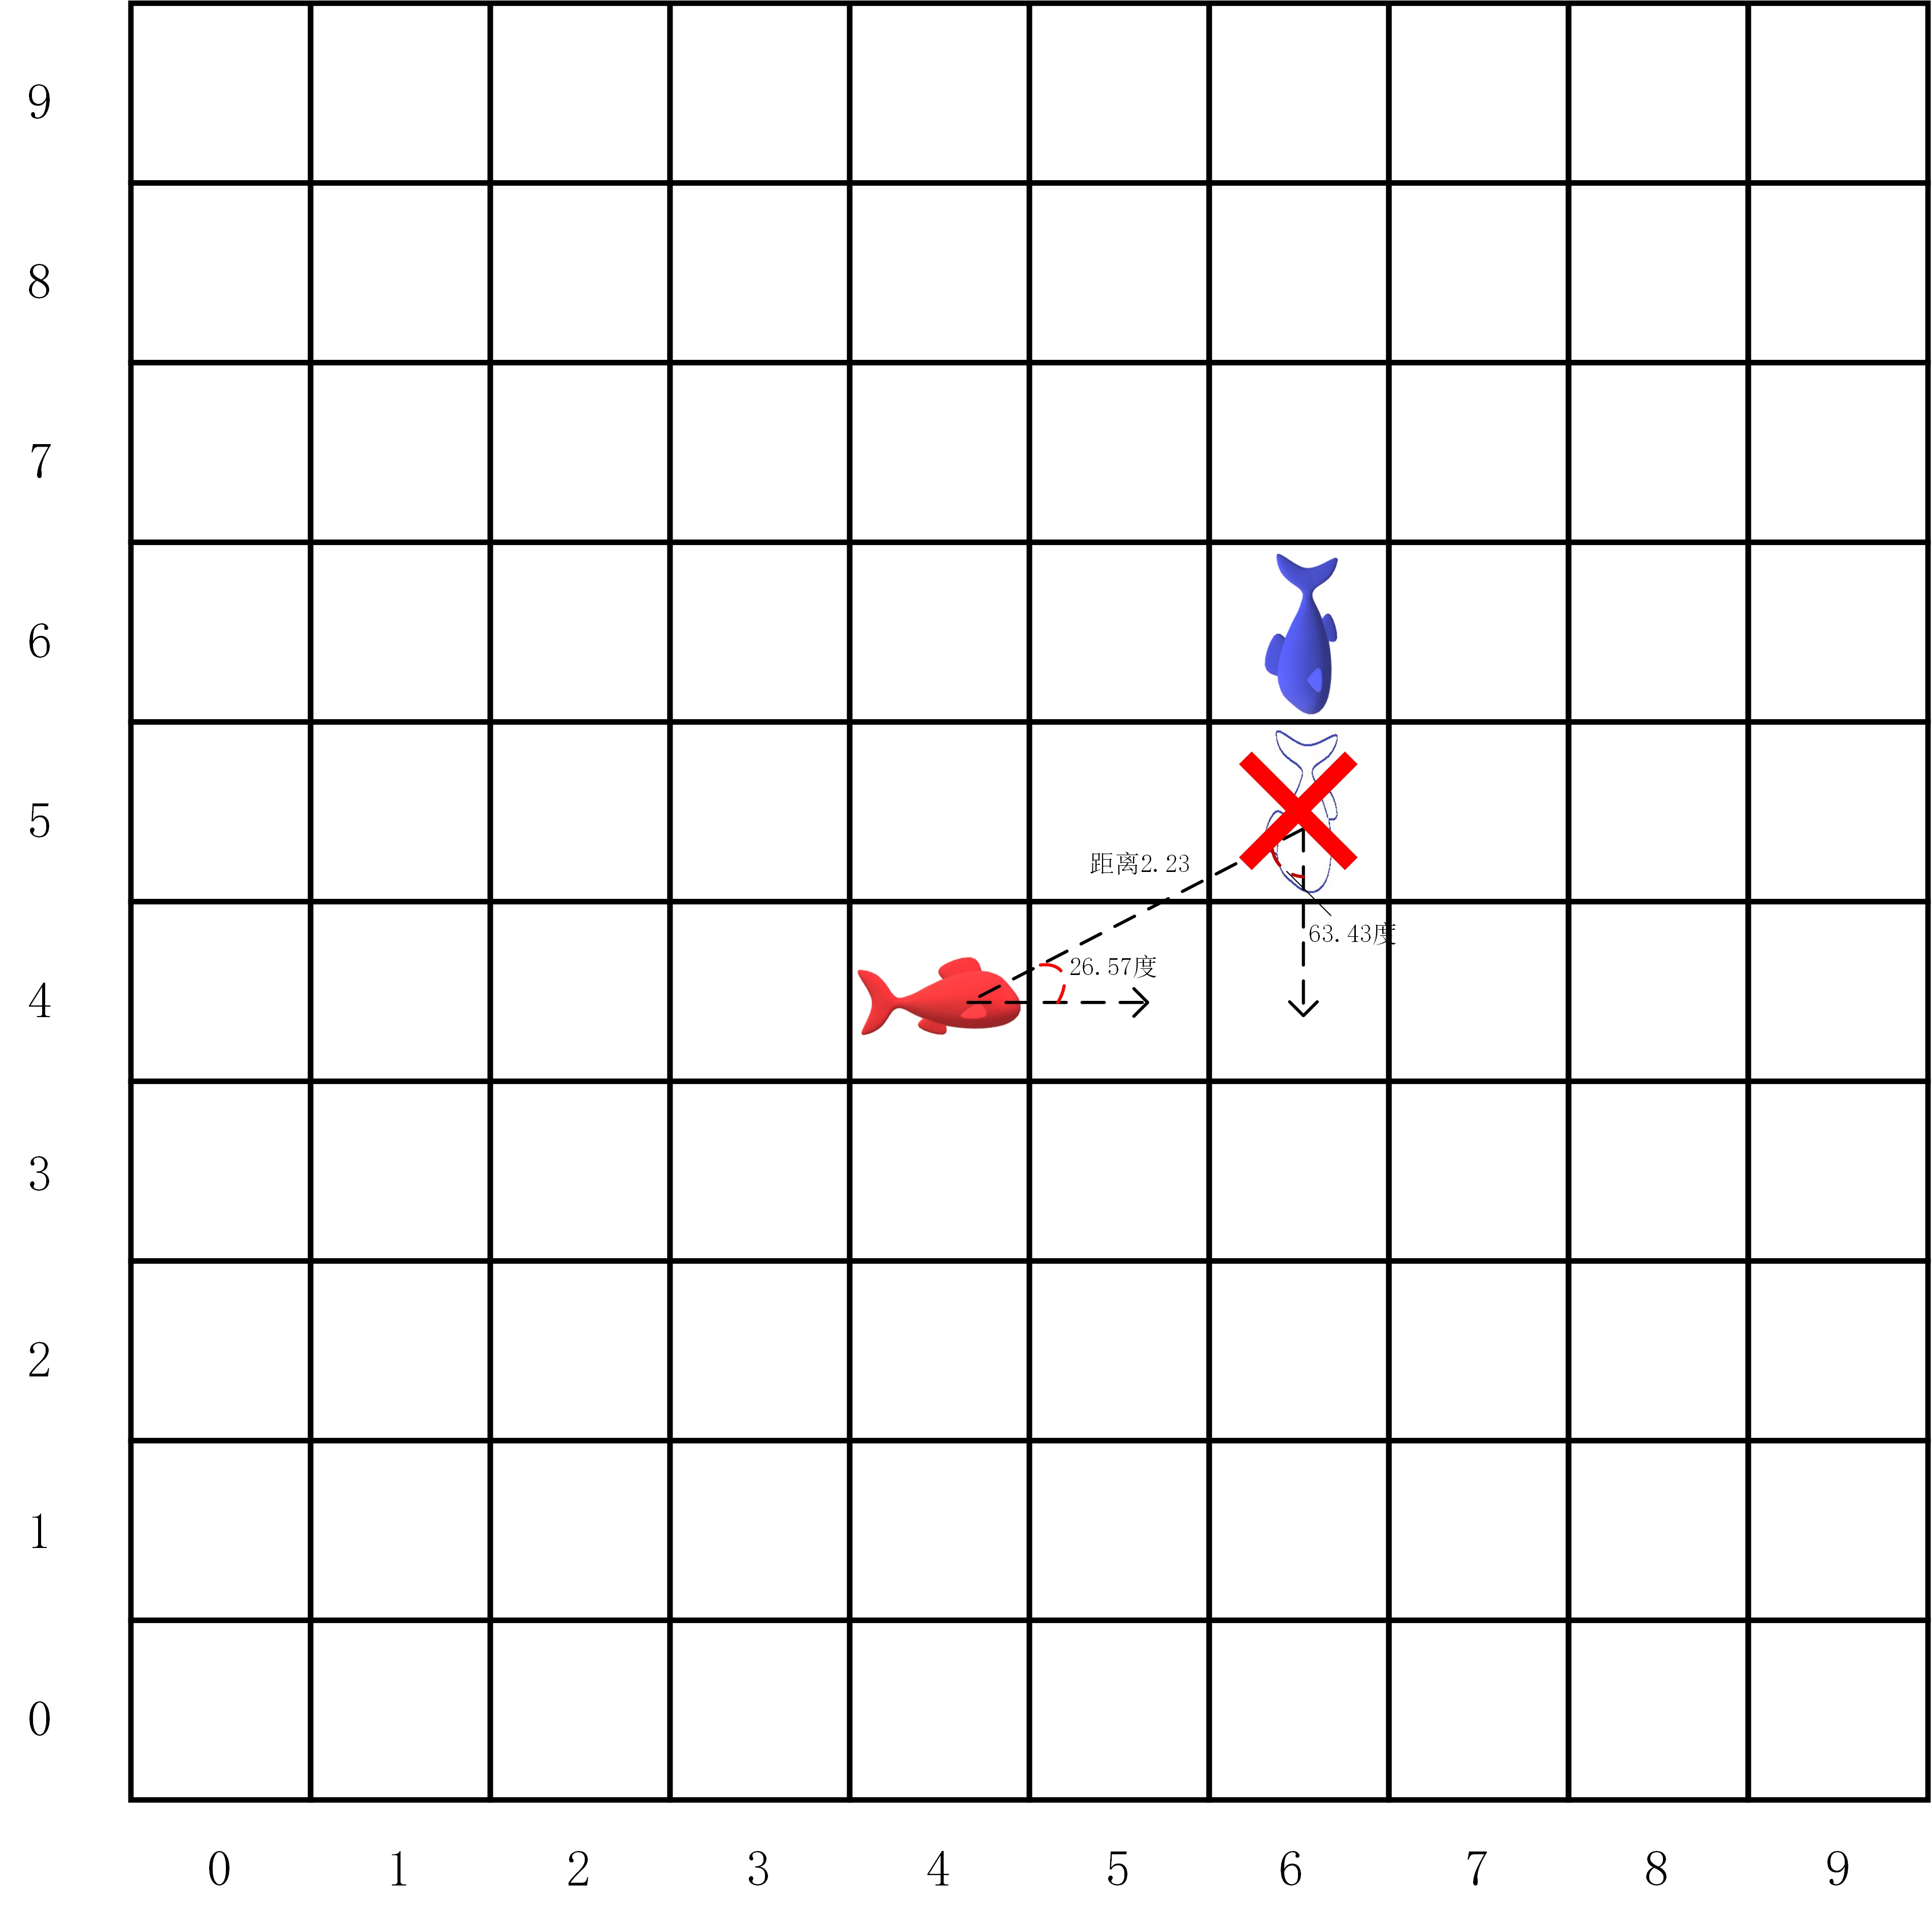
\includegraphics[width=0.45\hsize,height=0.45\hsize]{example/yiduiyi8.jpg}}
	\newline
	\centering
	\subcaptionbox{向左双方状态\label{fig2:yiduiyi7-10:c}}
	{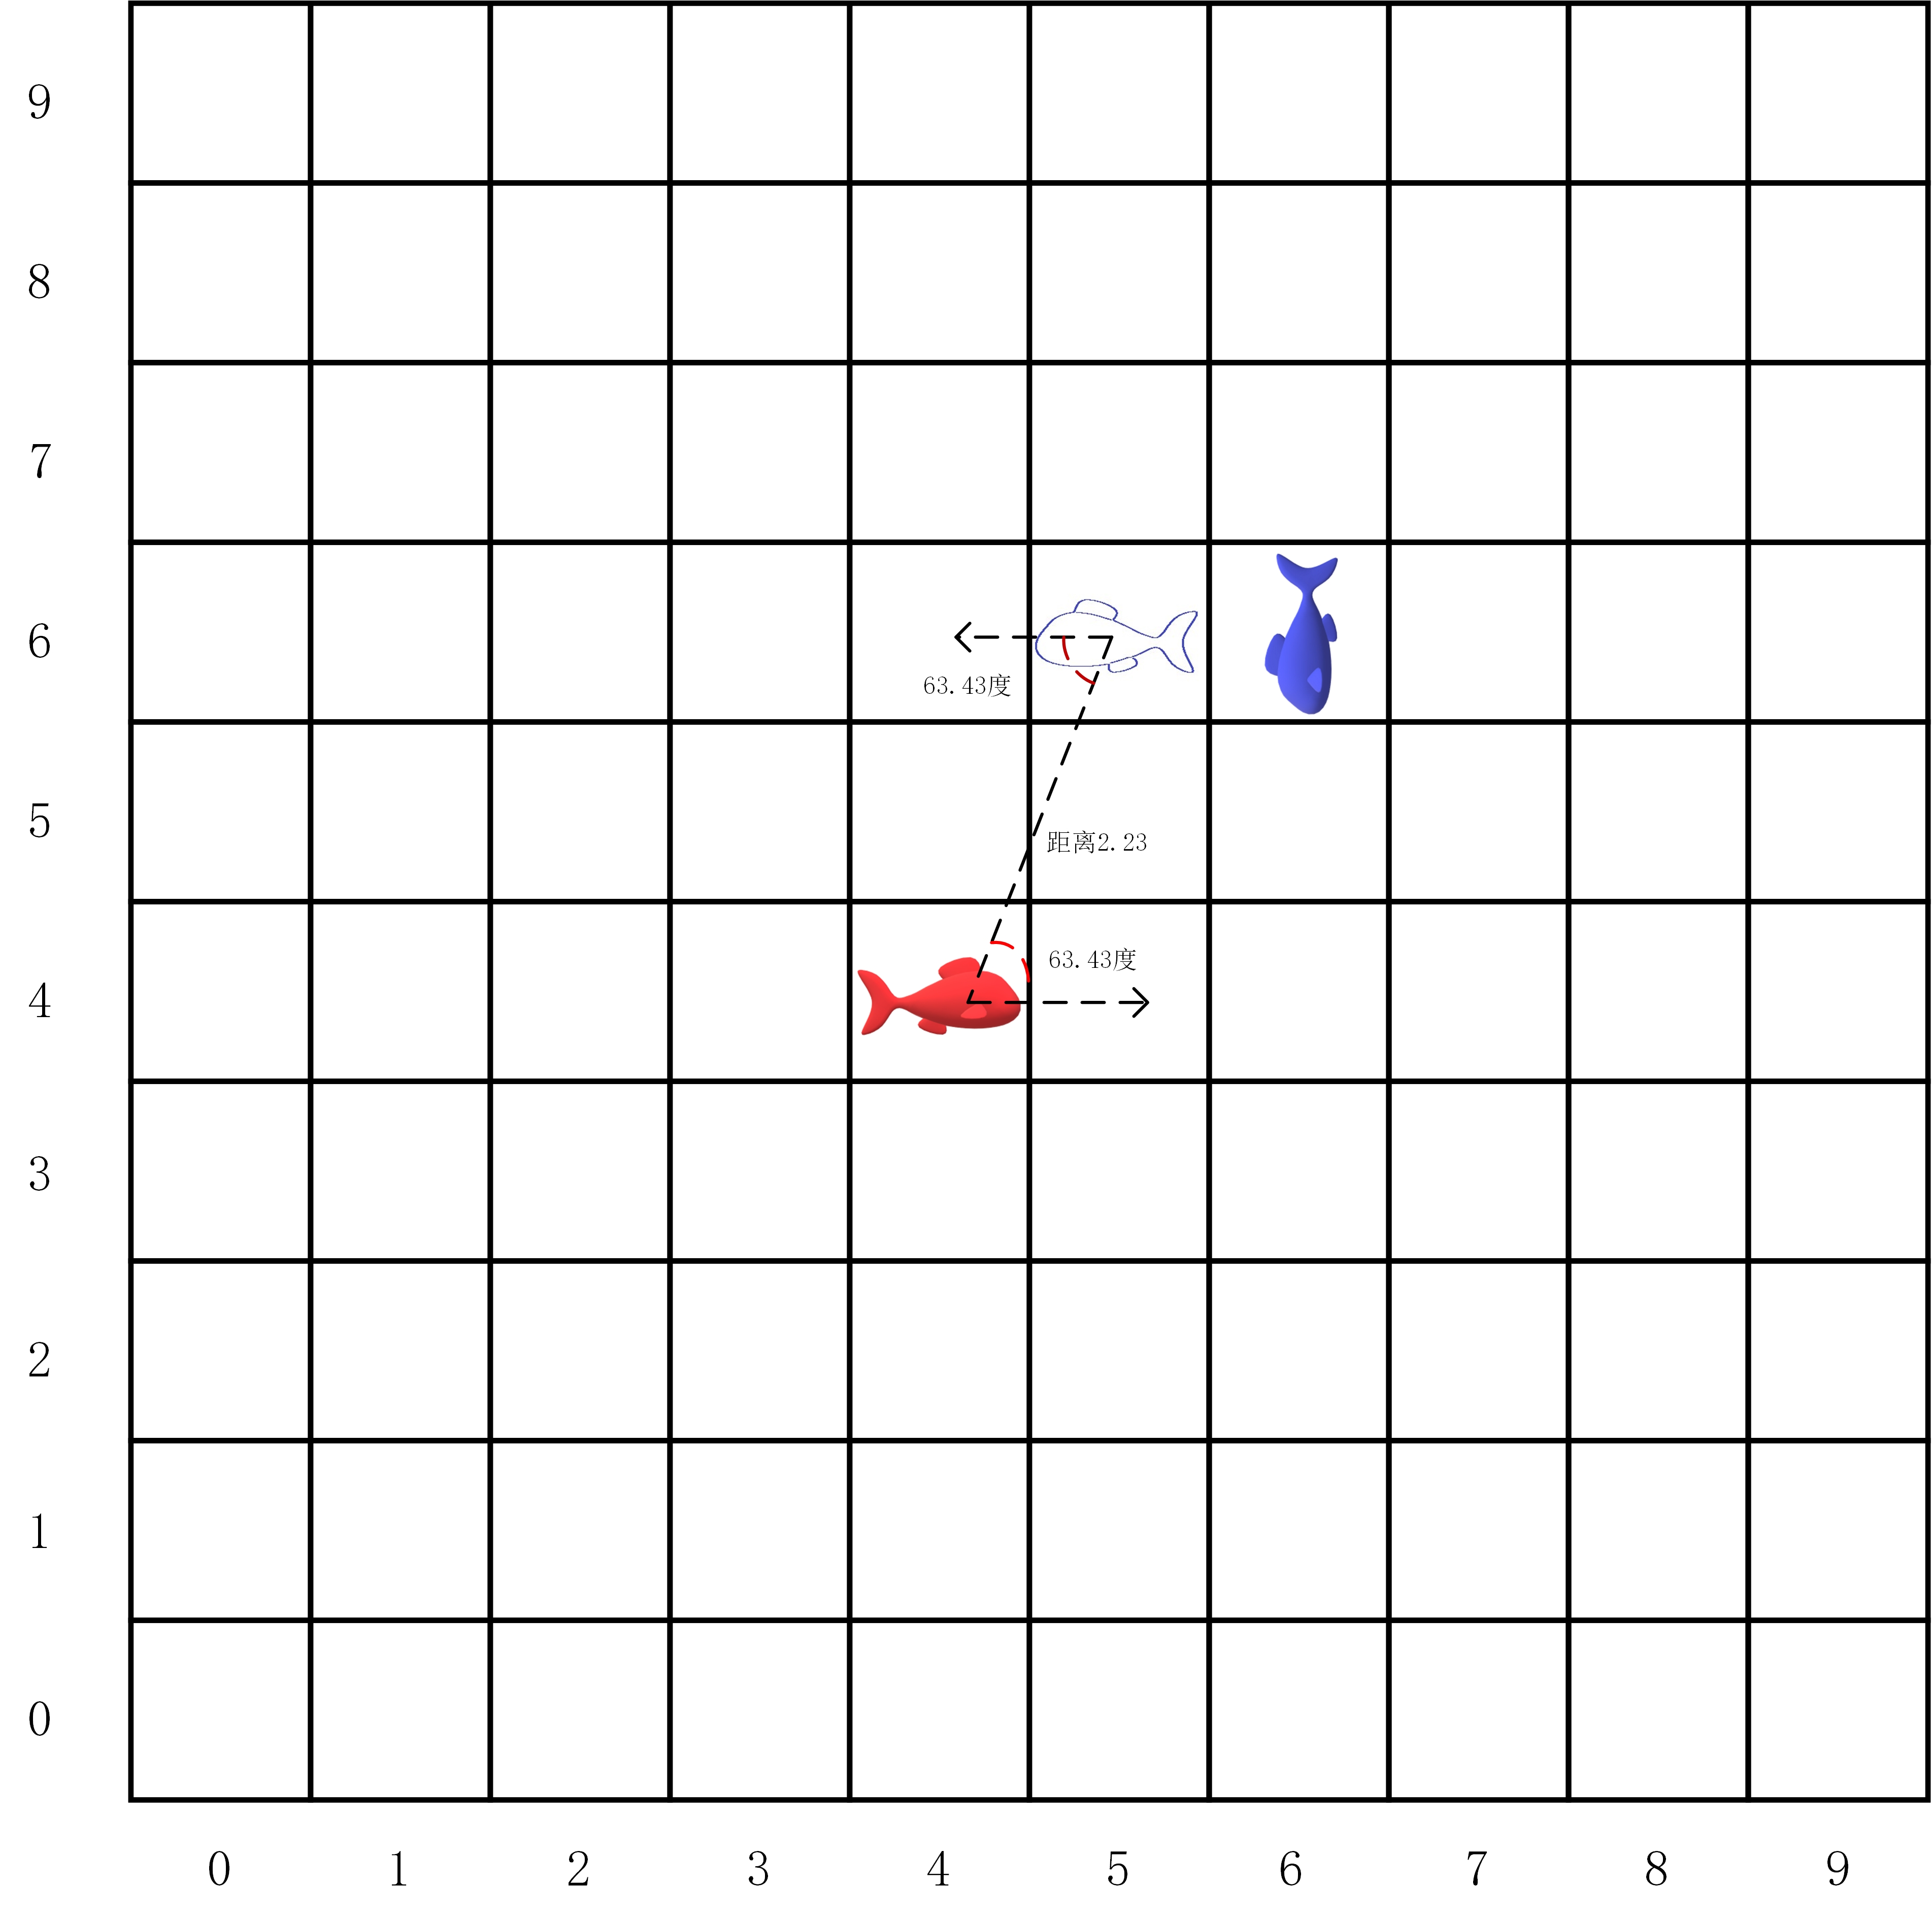
\includegraphics[width=0.45\hsize,height=0.45\hsize]{example/yiduiyi9.jpg}}
	\hspace{0.5em}
	\subcaptionbox{向右双方状态\label{fig2:yiduiyi7-10:d}}
	{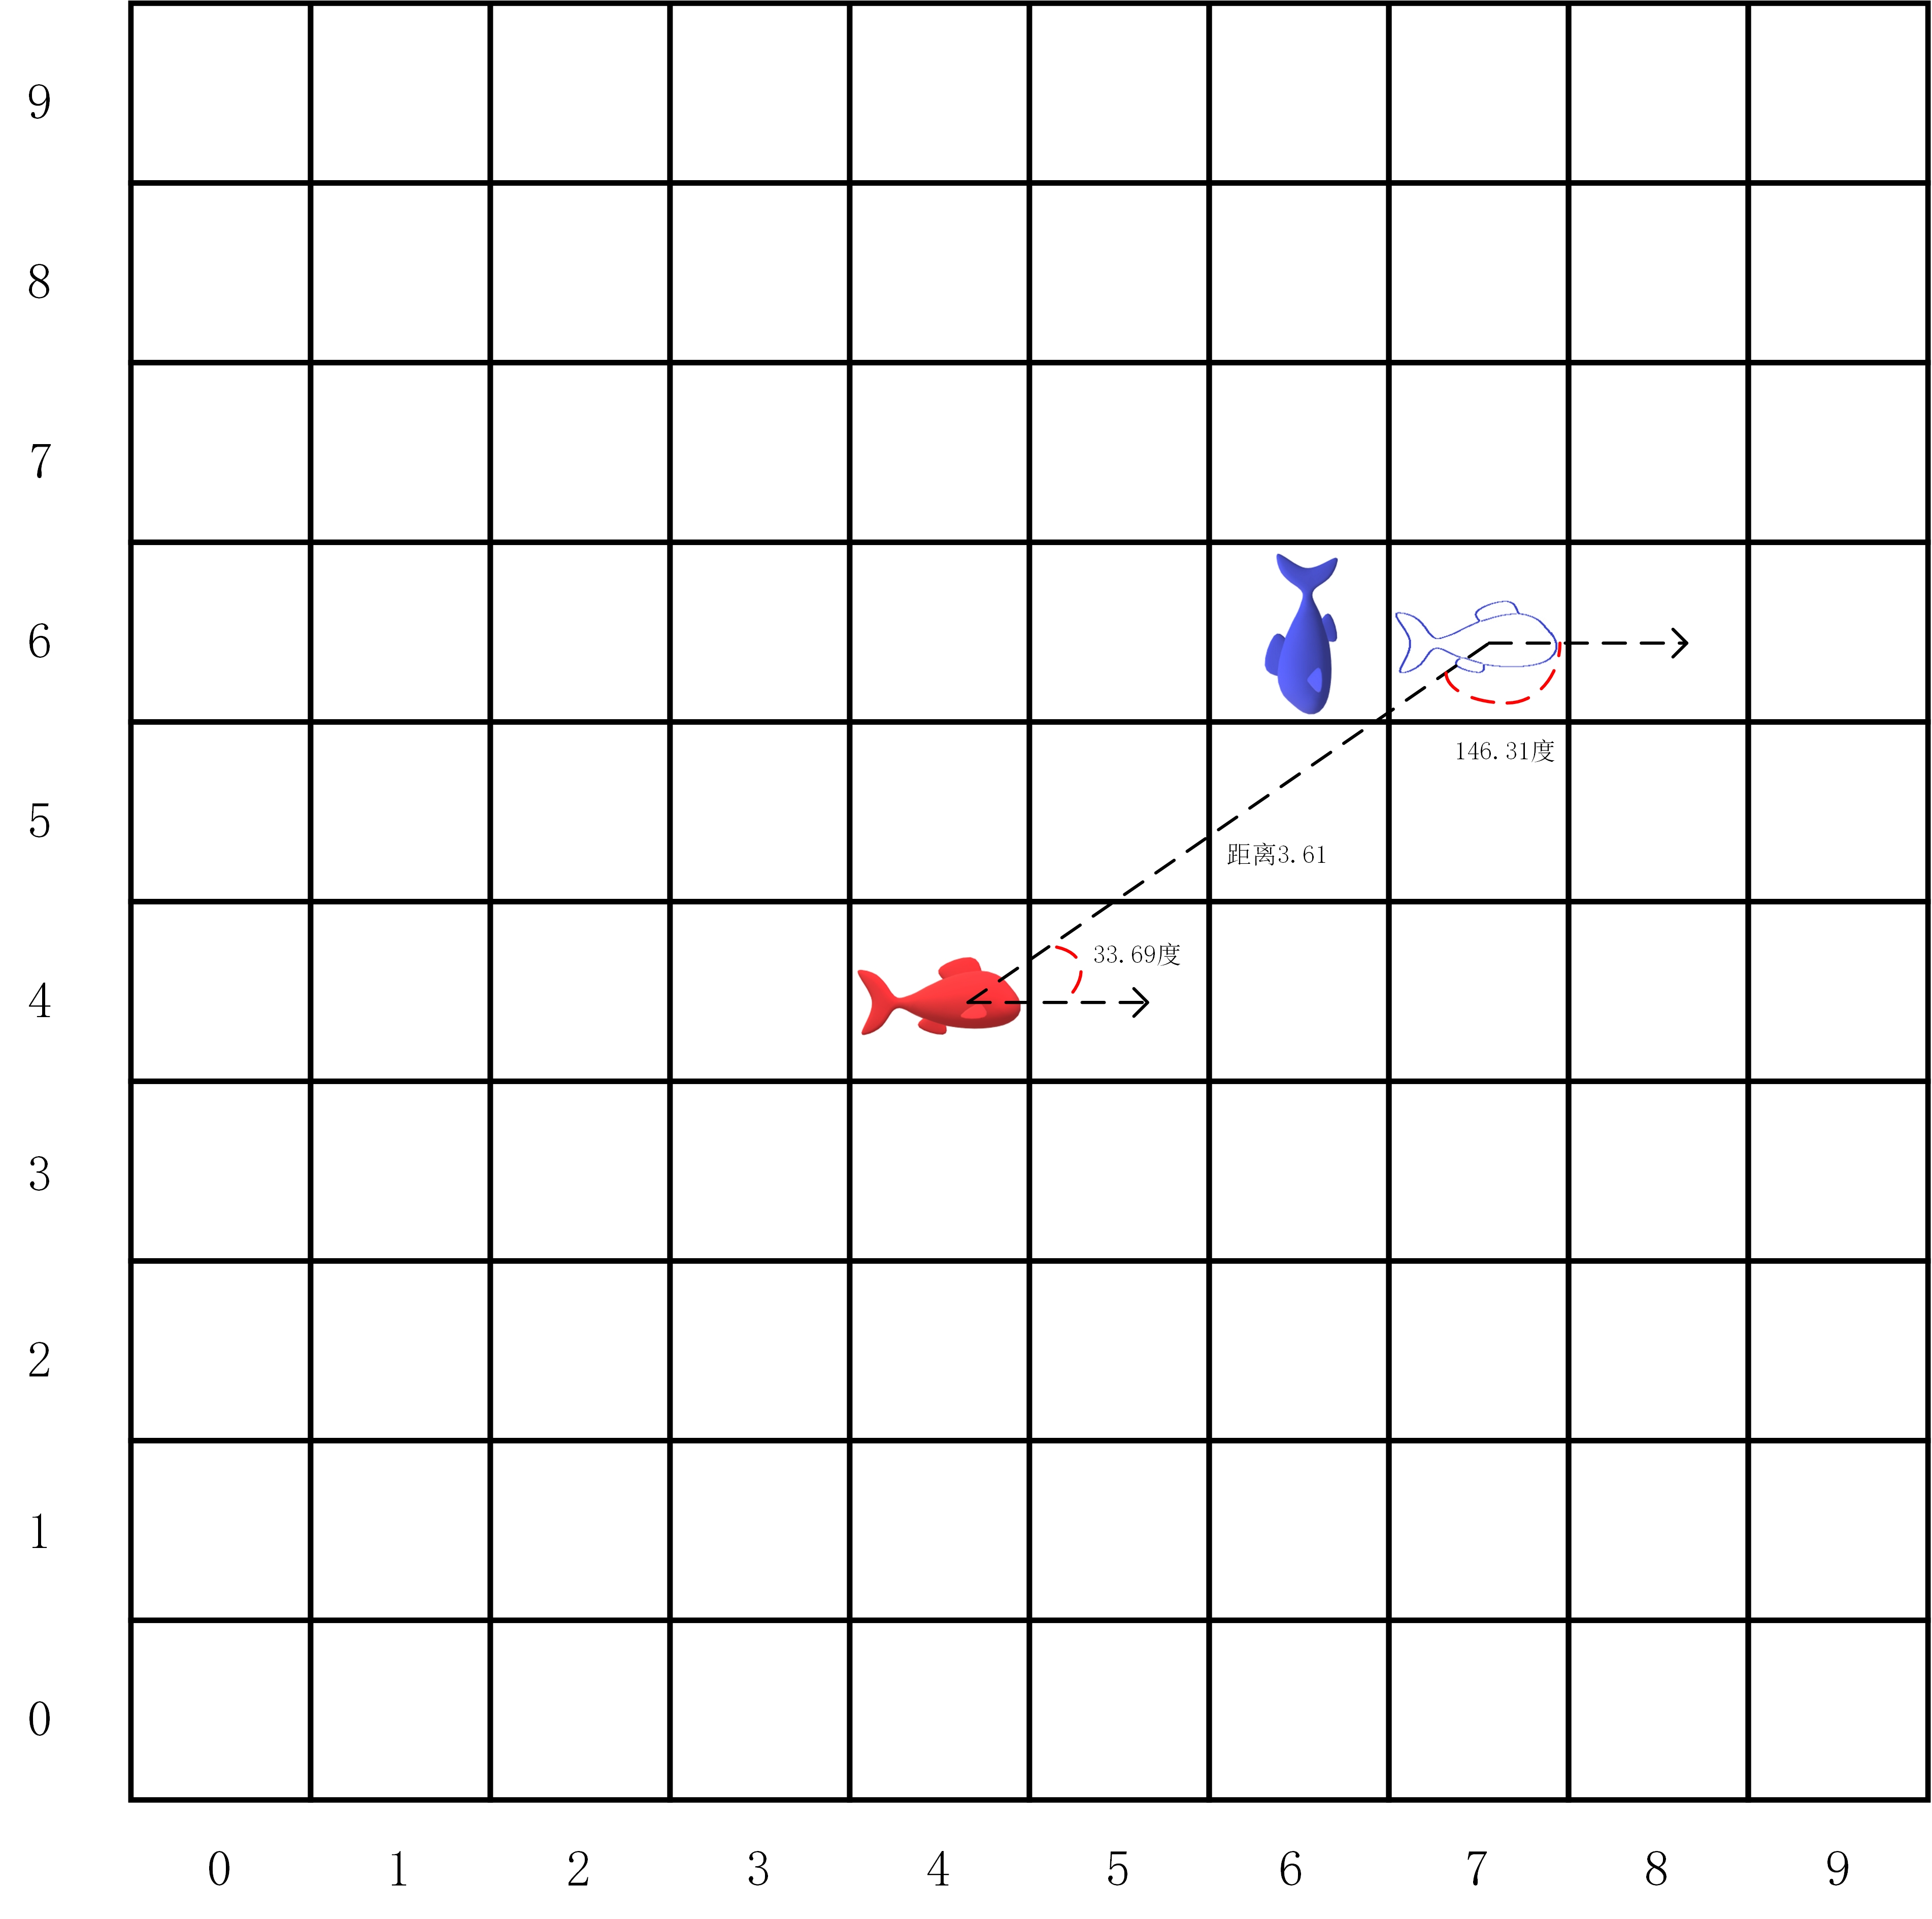
\includegraphics[width=0.45\hsize,height=0.45\hsize]{example/yiduiyi10.jpg}}
	\bicaption
	{一对一人机对弈状态分析}
	{Examples of response maps during occlusions and not.The first row shows the original and response maps with no occlusions while the second row shows the maps with occlusions. The first column are the shots of sequence bear front in Princeton dataset. The color response maps are in the second column while the depth’s are in the third.}
	\label{fig2:yiduiyi7-10}
\end{figure}
可以看出当蓝方向下走时,会被红方吃掉,对模型搜索得到的概率为0.0375。在\ref{fig2:yiduiyi3-6:c}状态时,对于蓝方执行四个动作进行分析:

\begin{figure}[!htpb]
	\centering
	\subcaptionbox{向上双方状态\label{fig2:yiduiyi11-14:a}}
	{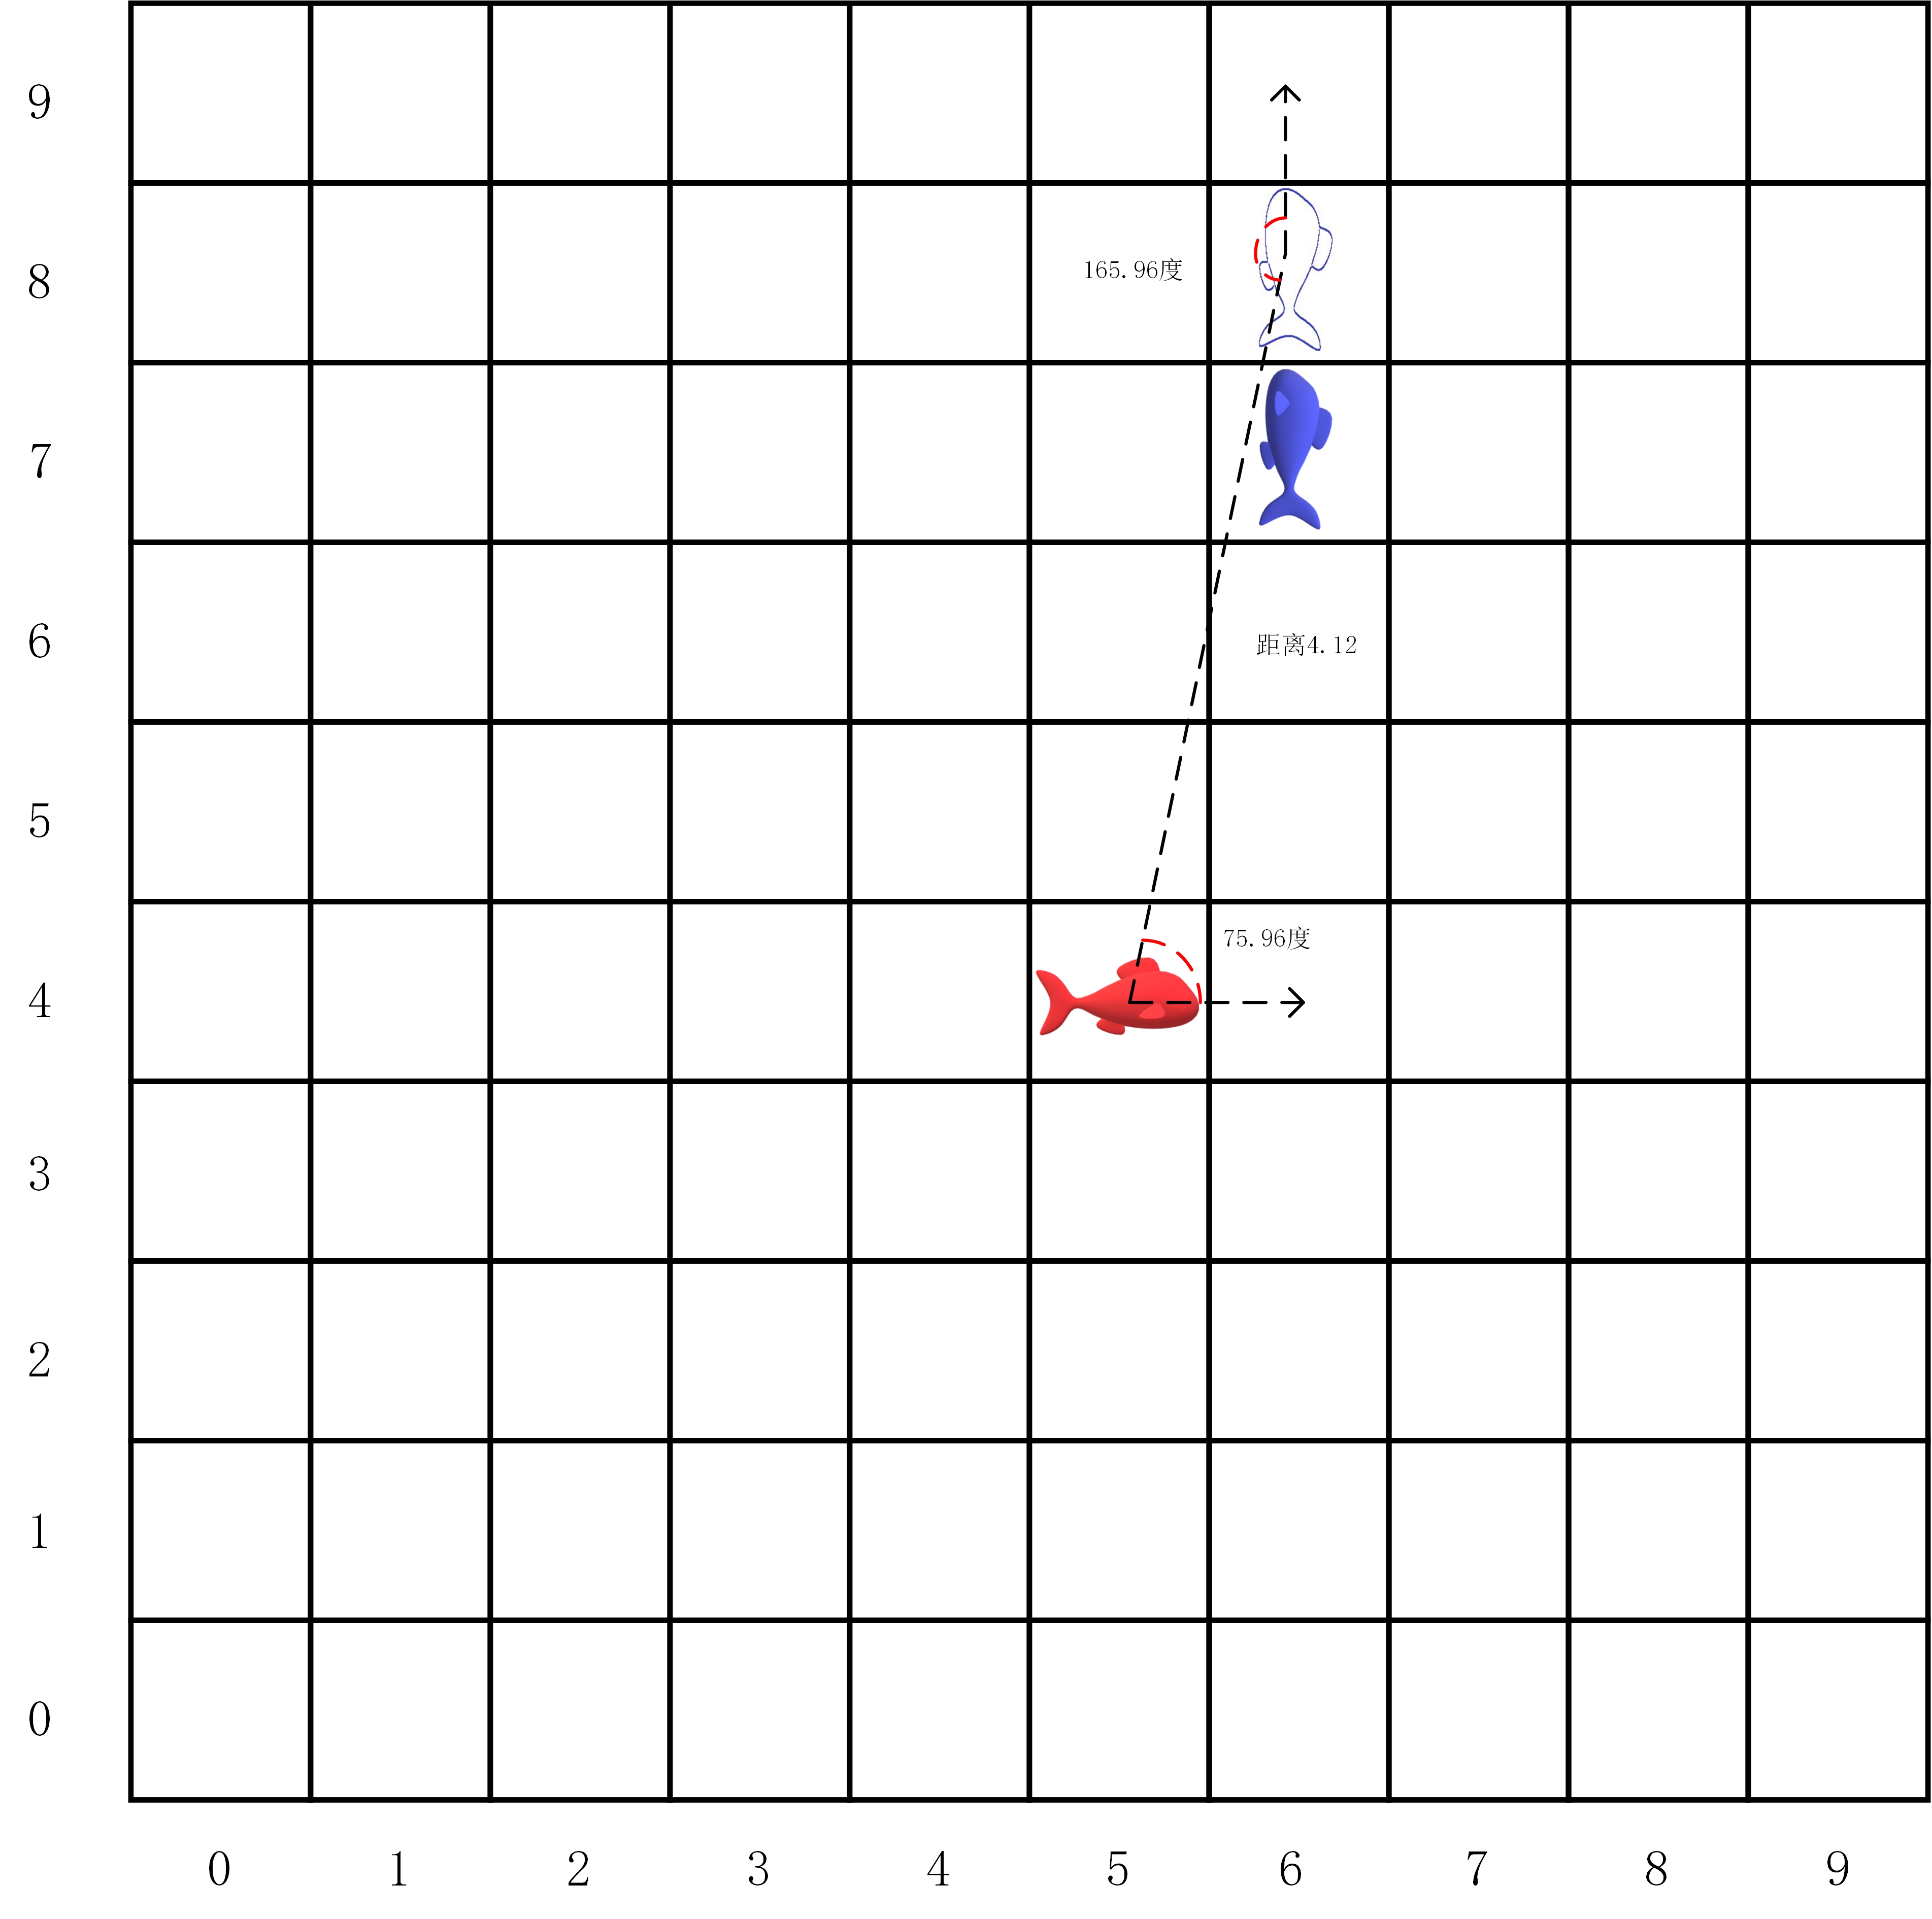
\includegraphics[width=0.45\hsize,height=0.45\hsize]{example/yiduiyi11.jpg}}
	\hspace{0.5em}
	\subcaptionbox{向下双方状态\label{fig2:yiduiyi11-14:b}}
	{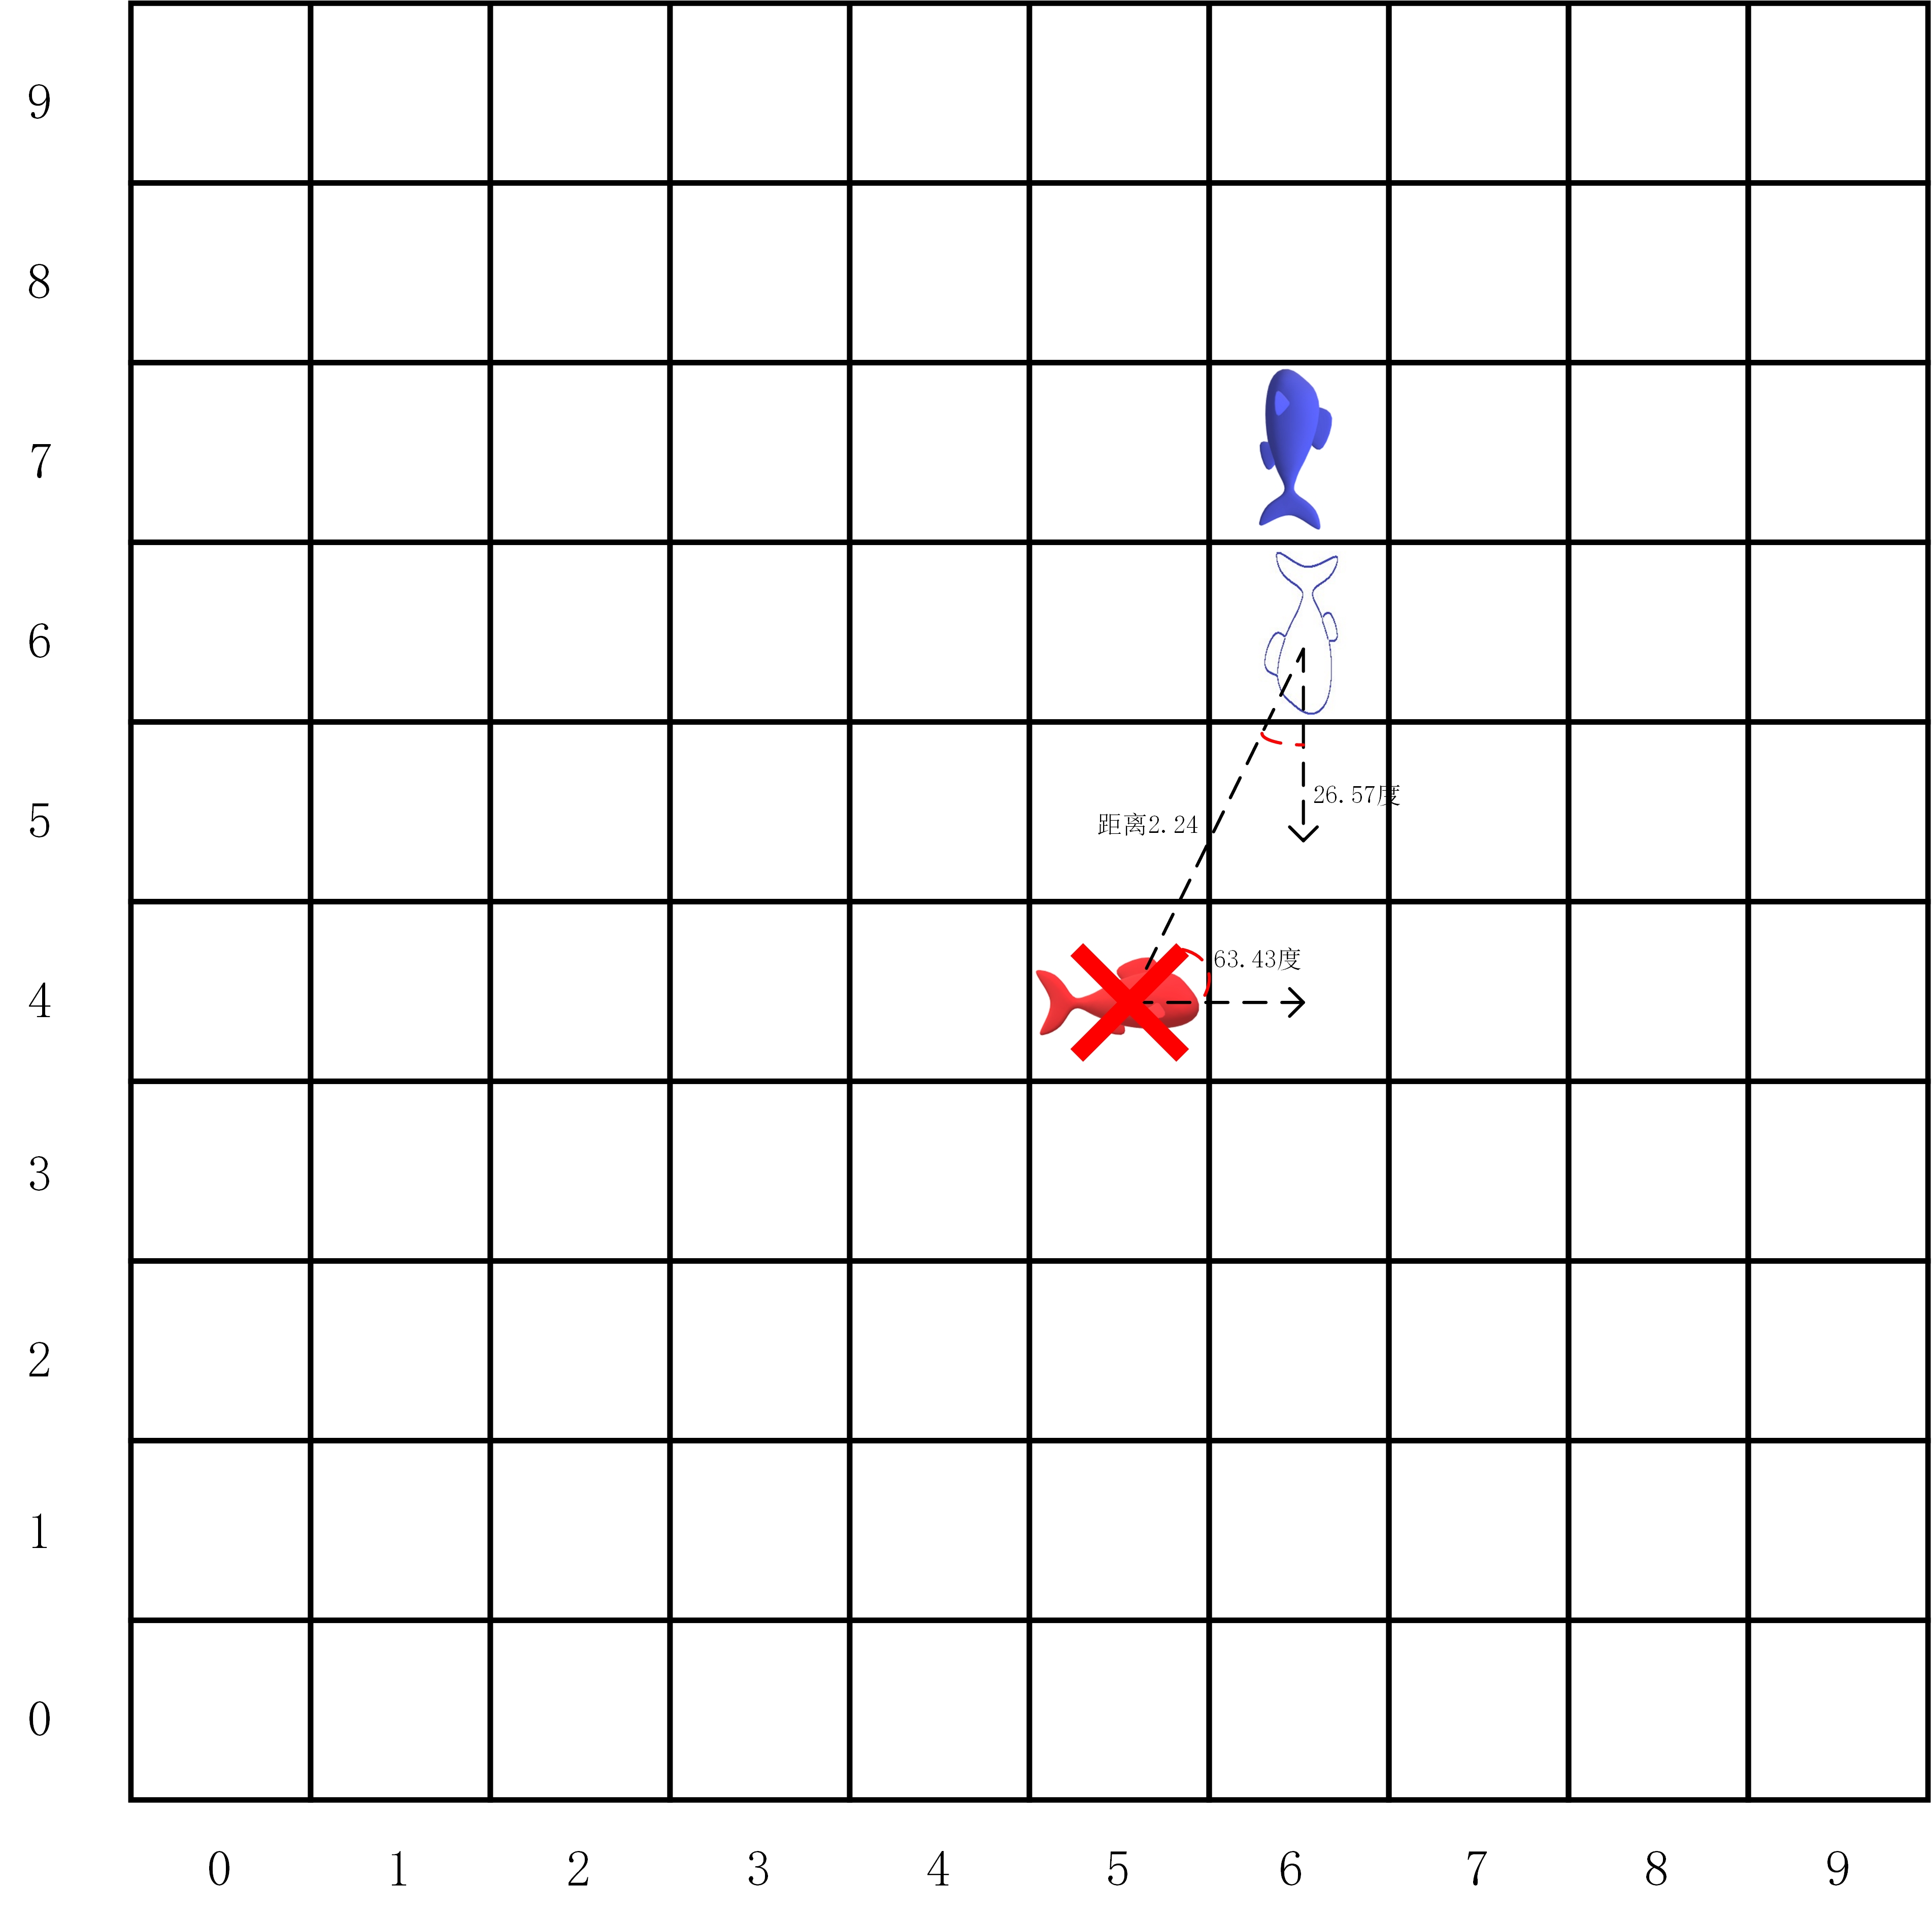
\includegraphics[width=0.45\hsize,height=0.45\hsize]{example/yiduiyi12.jpg}}
	\newline
	\centering
	\subcaptionbox{向左双方状态\label{fig2:yiduiyi11-14:c}}
	{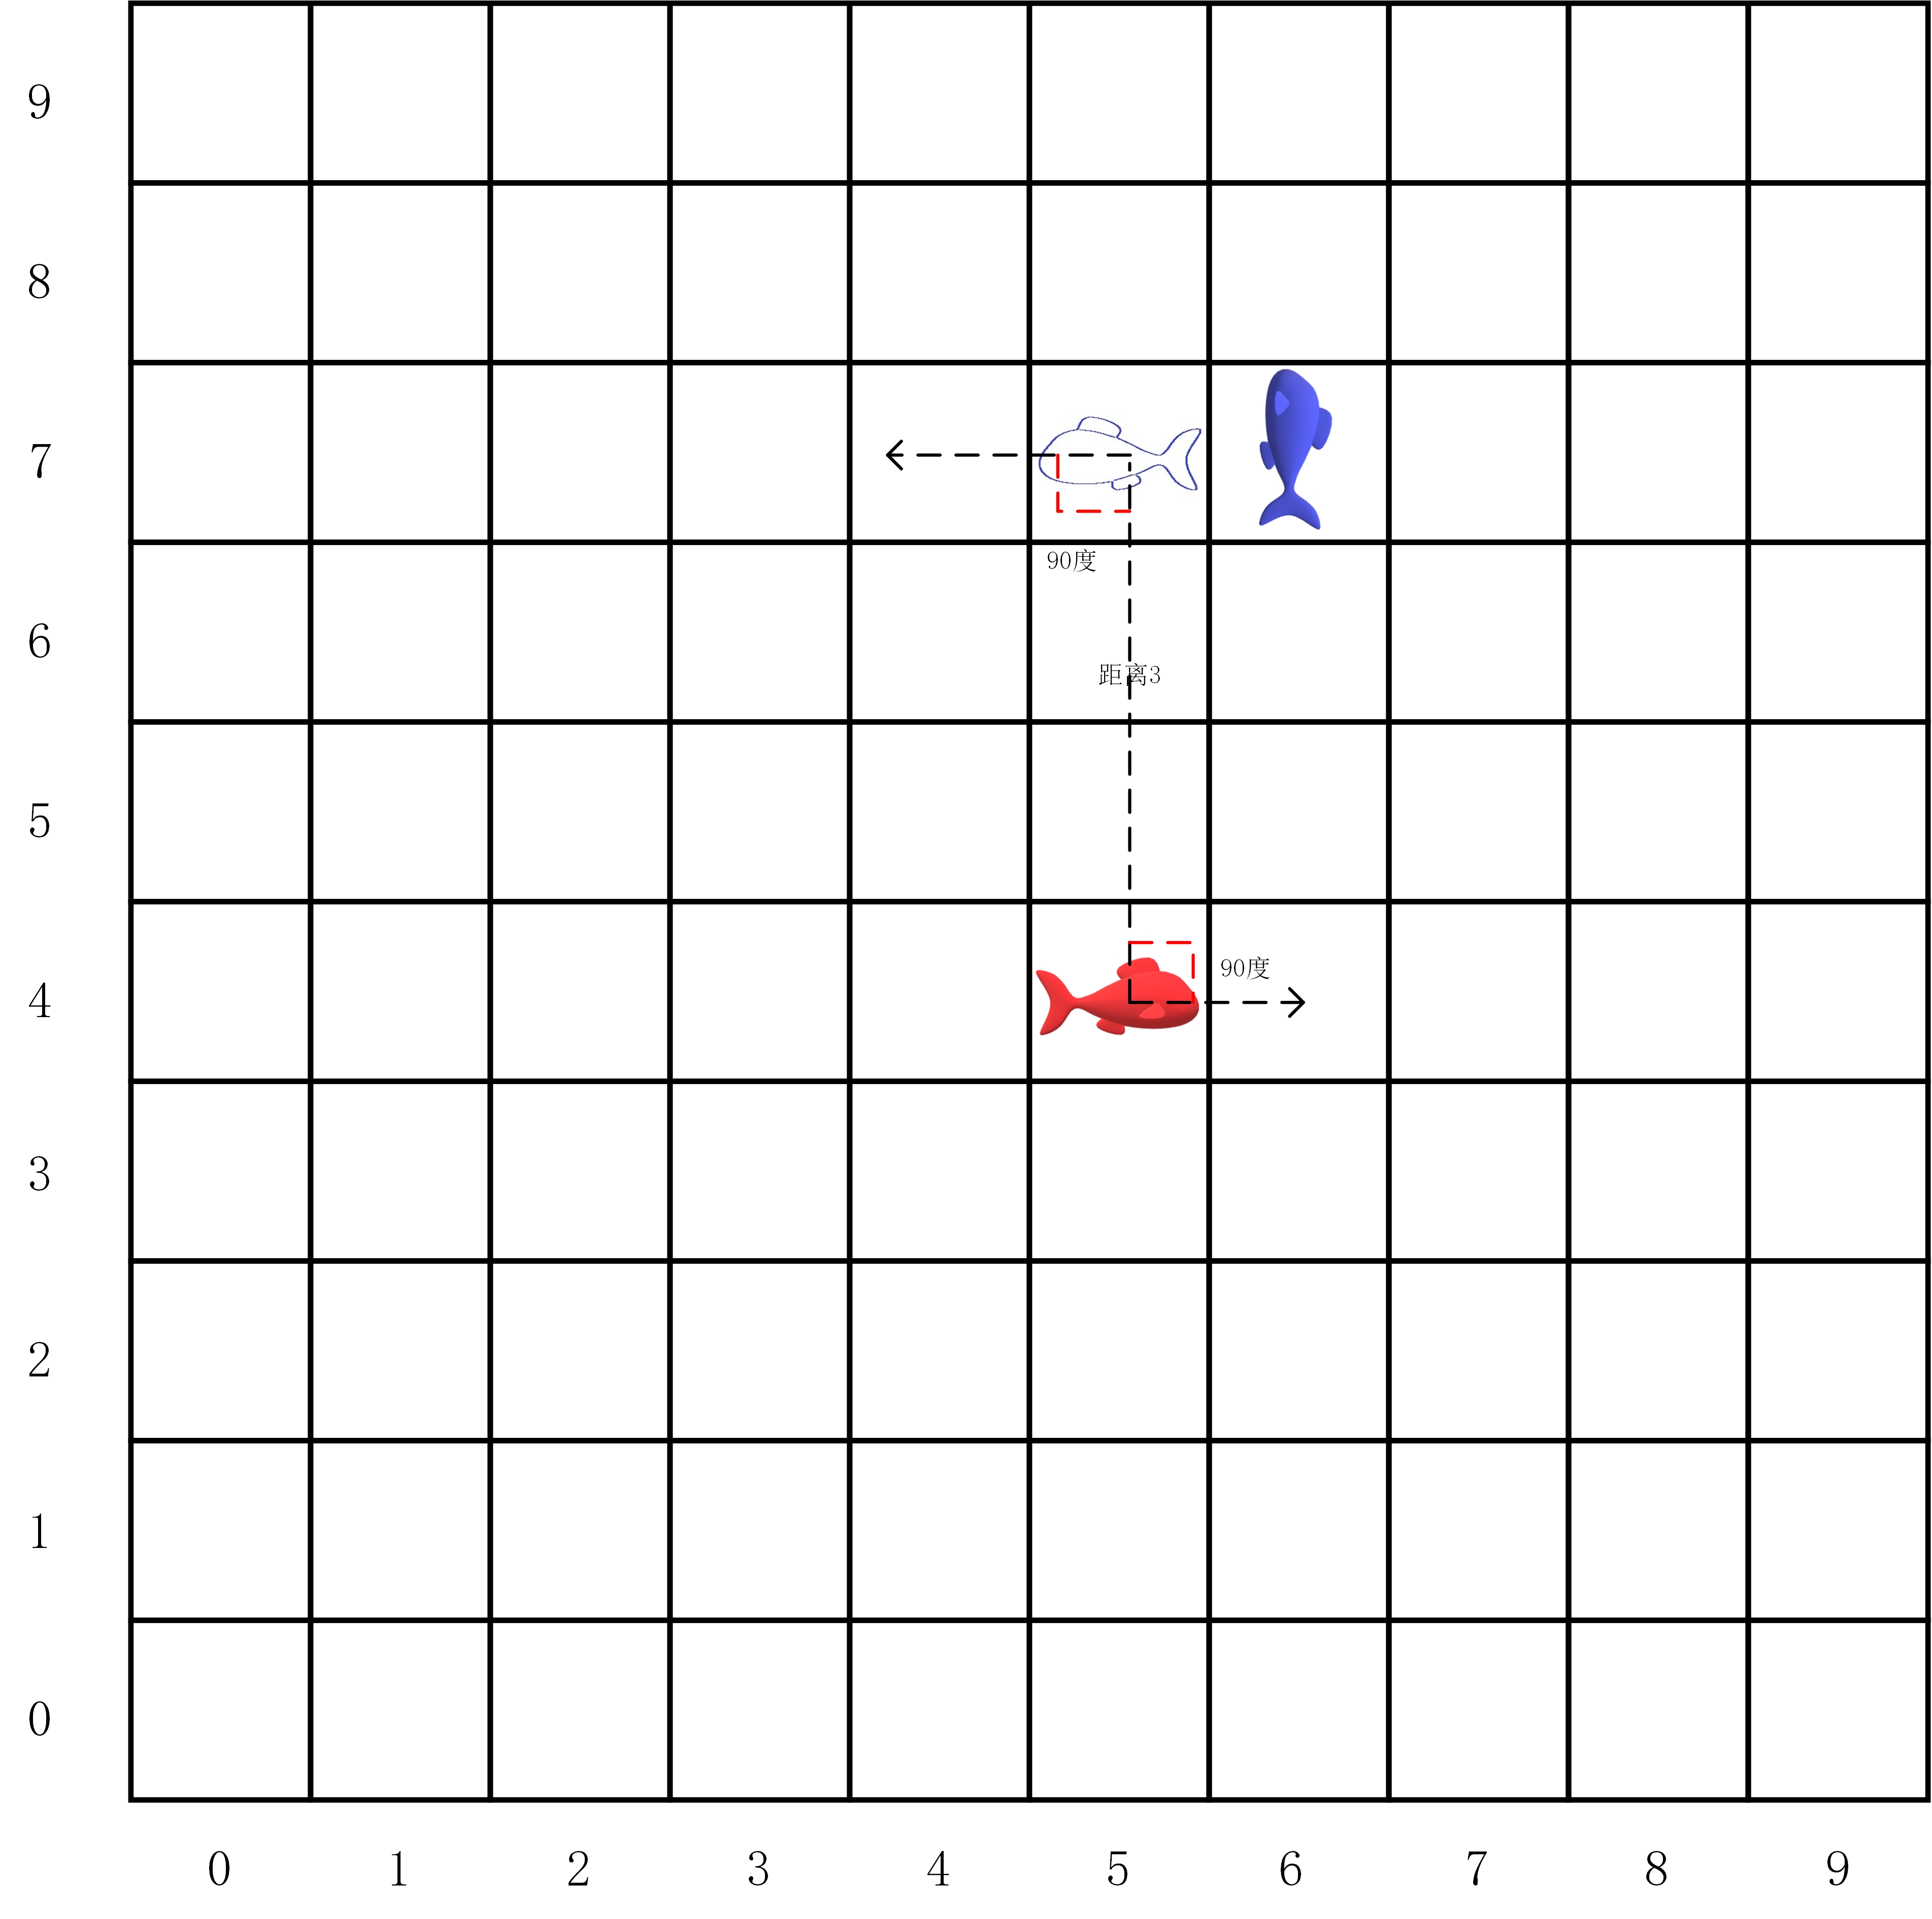
\includegraphics[width=0.45\hsize,height=0.45\hsize]{example/yiduiyi13.jpg}}
	\hspace{0.5em}
	\subcaptionbox{向右双方状态\label{fig2:yiduiyi11-14:d}}
	{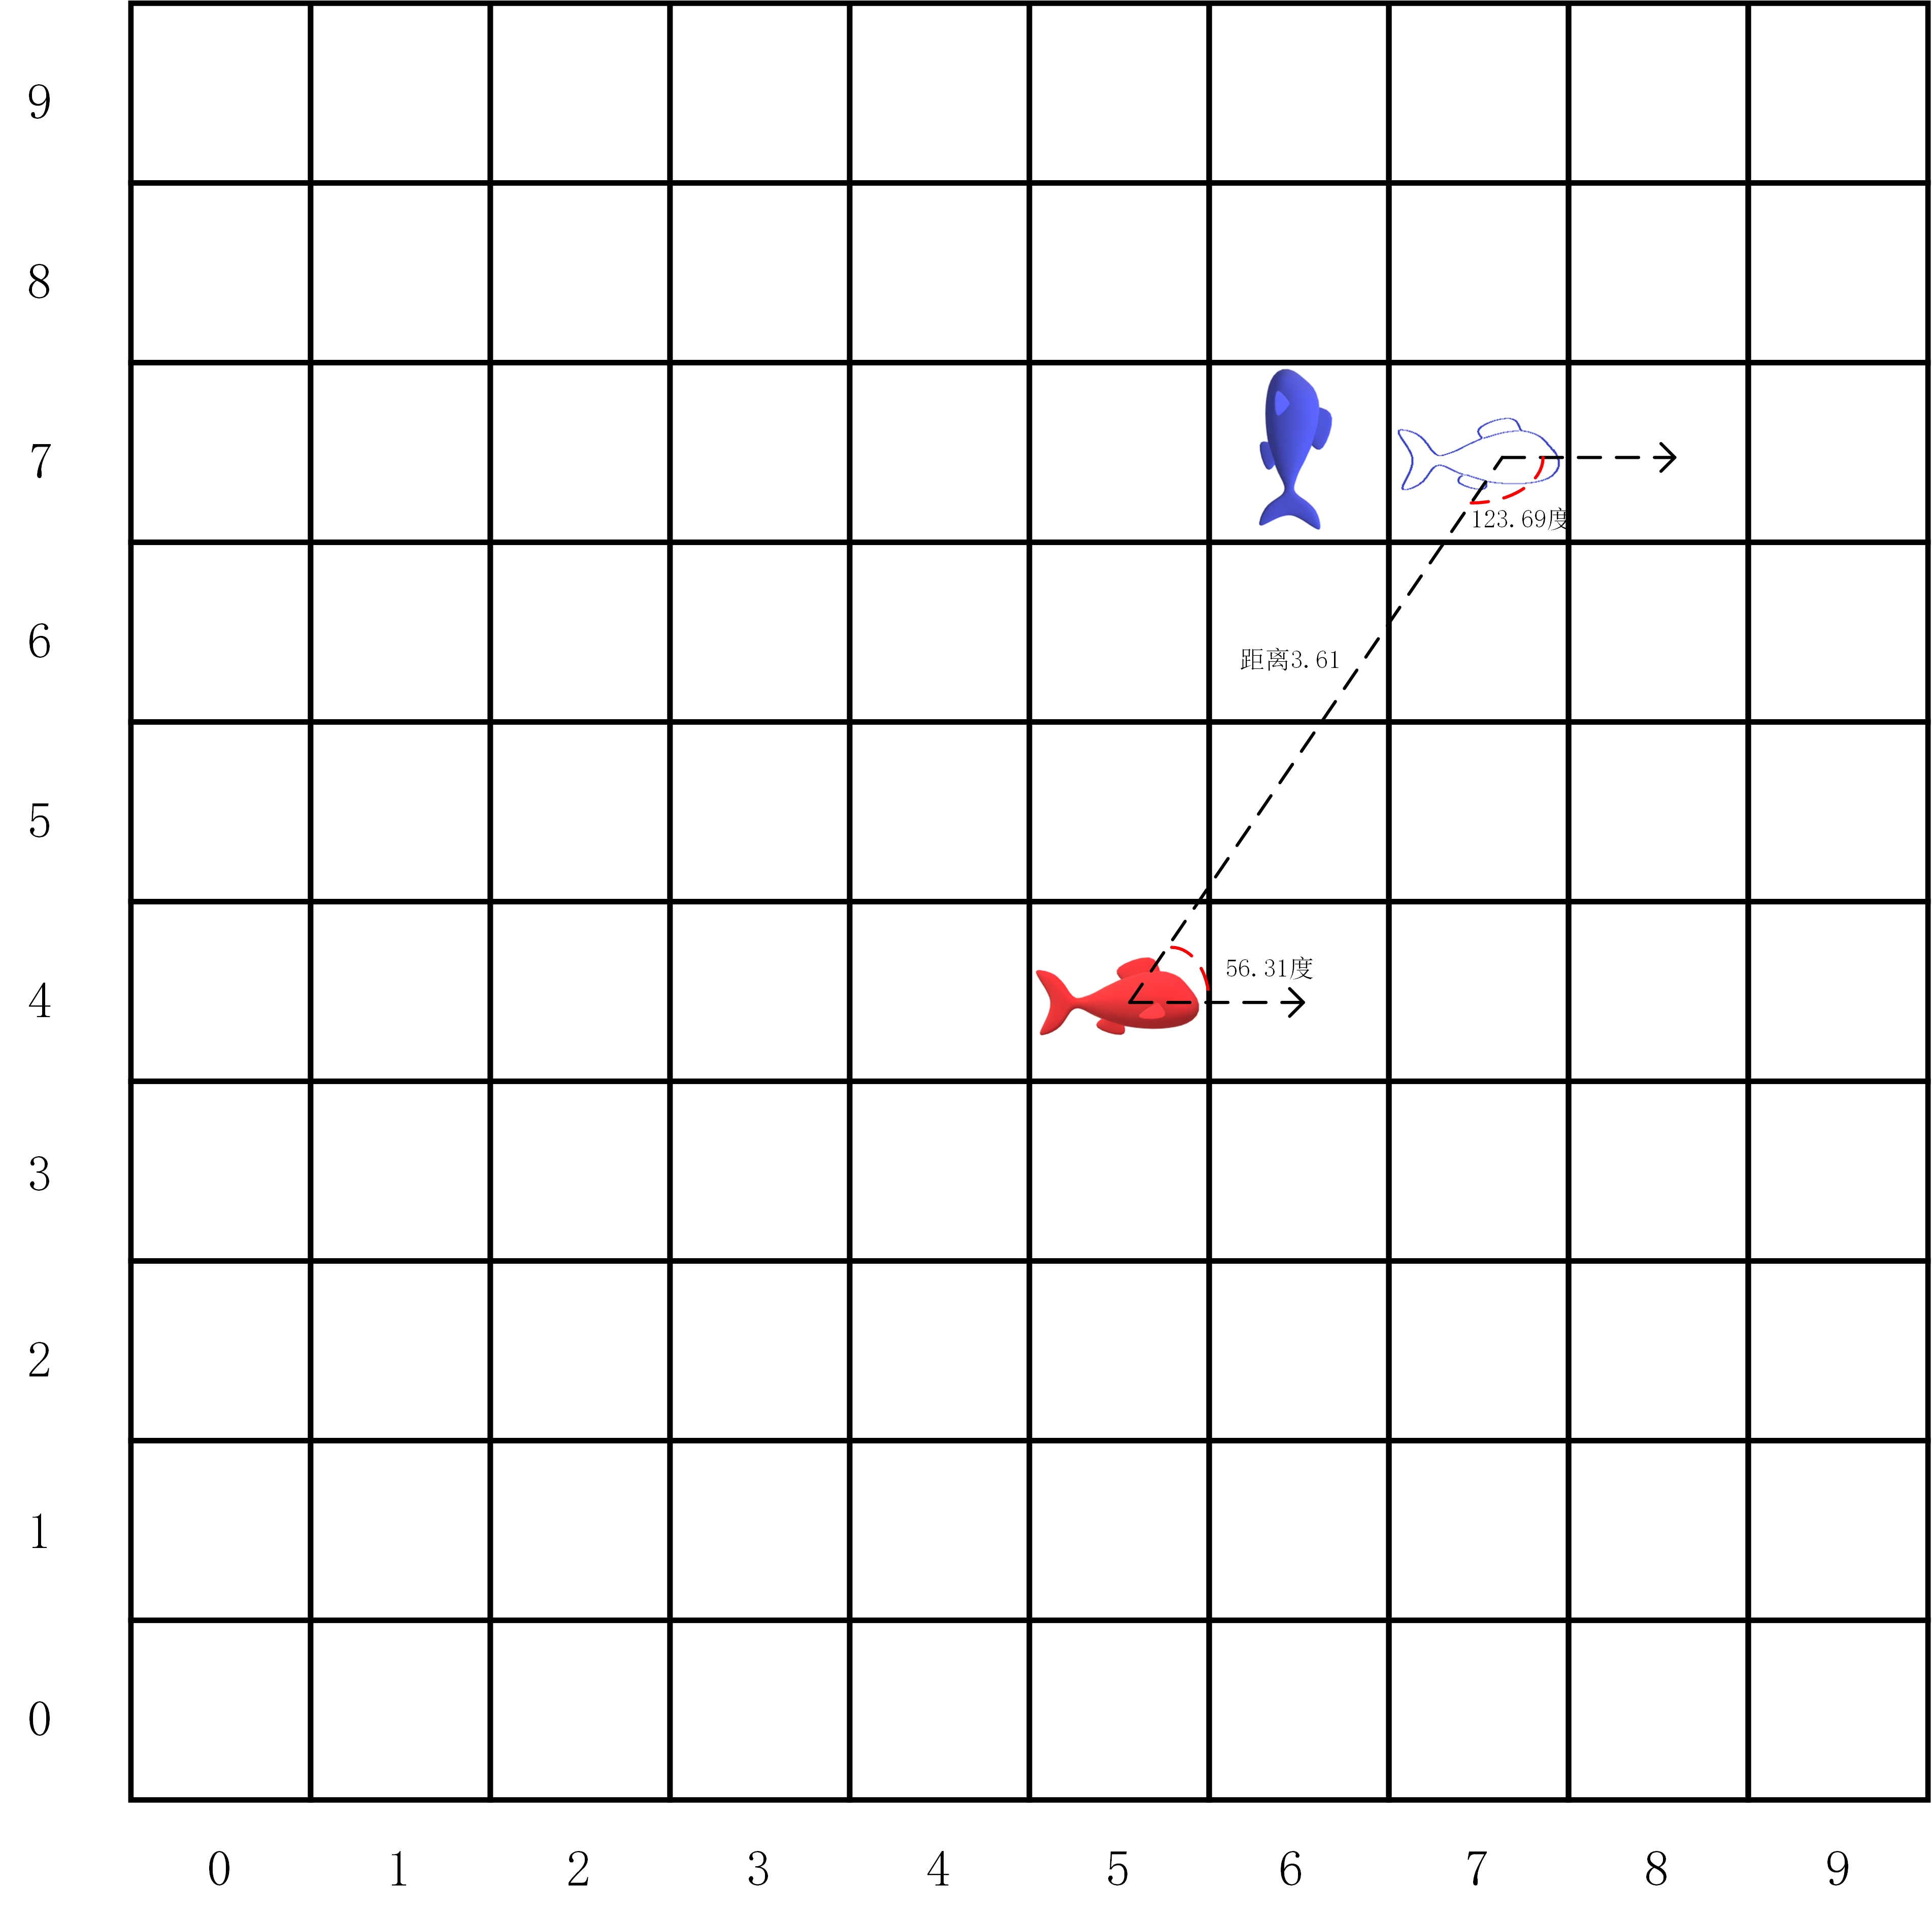
\includegraphics[width=0.45\hsize,height=0.45\hsize]{example/yiduiyi14.jpg}}
	\bicaption
	{一对一人机对弈状态分析}
	{Examples of response maps during occlusions and not.The first row shows the original and response maps with no occlusions while the second row shows the maps with occlusions. The first column are the shots of sequence bear front in Princeton dataset. The color response maps are in the second column while the depth’s are in the third.}
	\label{fig2:yiduiyi11-14}
\end{figure}
可见当蓝方向下时会把红方吃掉,对照模型搜索得到的概率,向下的概率最大,为0.755。

从一对一结果分析可以看出训练后的模型已经能识别出在那种状态应该远离敌方,并在合适的位置进行攻击。



\subsection{多对多实验结果}
在多对多实验中,参数设置如下:
\begin{table}
	\centering
	\caption{多对多实验参数信息}
	\begin{tabular}{c|c}
		\hline 
		棋盘大小 & 10*10 \\ 
		\hline 
		自适应学习率参数$\lambda$ & 1.5 \\ 
		\hline 
		温度探索参数$\tau$& 1.0 \\ 
		\hline 
		每次落子蒙特卡洛搜索次数 & 500 \\ 
		\hline 
		贪心策略$\epsilon$ & 0.75 \\ 
		\hline 
		起始学习率 & 2e-3
	\end{tabular} 
\end{table}
奖励设置为当双方各走完200步没有分出胜负,各奖励0,当一方至少有一条小鱼被吃掉,获胜方奖励为1,失败方奖励为-1。为了加快收敛速度,人为定义规则,当双方距离小于7时,只能向相互靠近的方向移动,对比加入规则前后得到的交叉熵和损失函数曲线为:
\begin{figure}[!bpt]
	\centering
	\subcaptionbox{规则对交叉熵的影响\label{fig1:guize:a}}
	{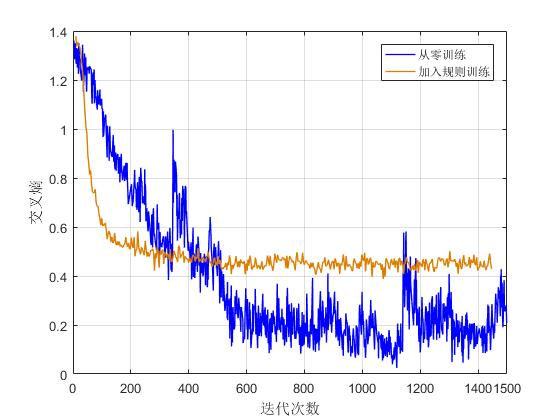
\includegraphics[width=0.45\hsize,height=0.45\hsize]{example/duoduiduoentropy.jpg}}
	\hspace{0.5em}
	\subcaptionbox{规则对损失函数的影响\label{fig1:guize:b}}
	{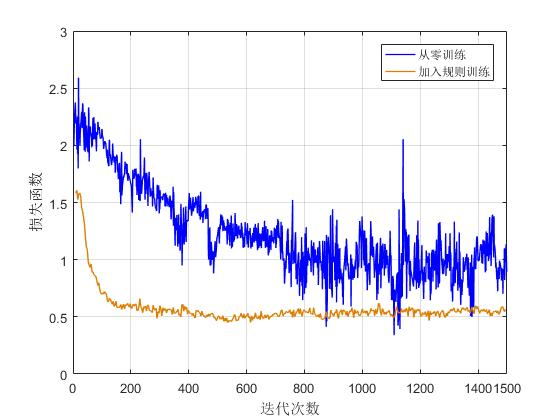
\includegraphics[width=0.45\hsize,height=0.45\hsize]{example/duoduiduoloss.jpg}}
	\bicaption
	{是否引入先验规则效果对比}
	{Examples of response maps during occlusions and not.The first row shows the original and response maps with no occlusions while the second row shows the maps with occlusions. The first column are the shots of sequence bear front in Princeton dataset. The color response maps are in the second column while the depth’s are in the third.}
	\label{fig1:guize}
\end{figure}
从\ref{fig1:guize:a}可以看出在训练初期加入规则之前交叉熵下降相对缓慢,加入规则之后在训练初期交叉熵下降较快,但是在后期交叉熵稳定在0.45左右,而不加规则的模型交叉熵还在持续下降。从\ref{fig1:guize:b}可以看出加入规则的模型损失函数相对容易学习,因为加入规则后人为干预了数据样本的多样性,所以网络更容易学习,但是同时失去了模型的泛化能力。利用加入规则的模型和没有加规则的模型分别在训练的前中后期进行50轮对弈。得到的对弈的结果如下:
\begin{figure}[!hbtp]
	\centering
	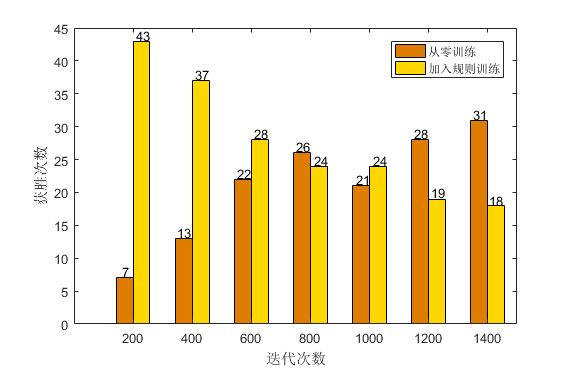
\includegraphics[width=10cm]{example/win.jpg}
	\bicaption[这里将出现在插图索引]
	{对弈统计结果}
	{Neural network training pipeline}
	\label{fig:win}
\end{figure}


人机对战结果展示如下:
在这里人类控制的红色小鱼先向上走一步,到达位置$(1,4)$计算红色小鱼对蓝色鱼和深蓝色鱼的位置信息,都没有被吃掉。轮到模型控制的深蓝色鱼进行动作,蓝色小鱼可行的位置为上,下和左,分别对应动作0,1,2。经过500次蒙特卡洛搜索树搜索得到各个位置的概率信息如下:
\begin{figure}[!htp]
	\centering
	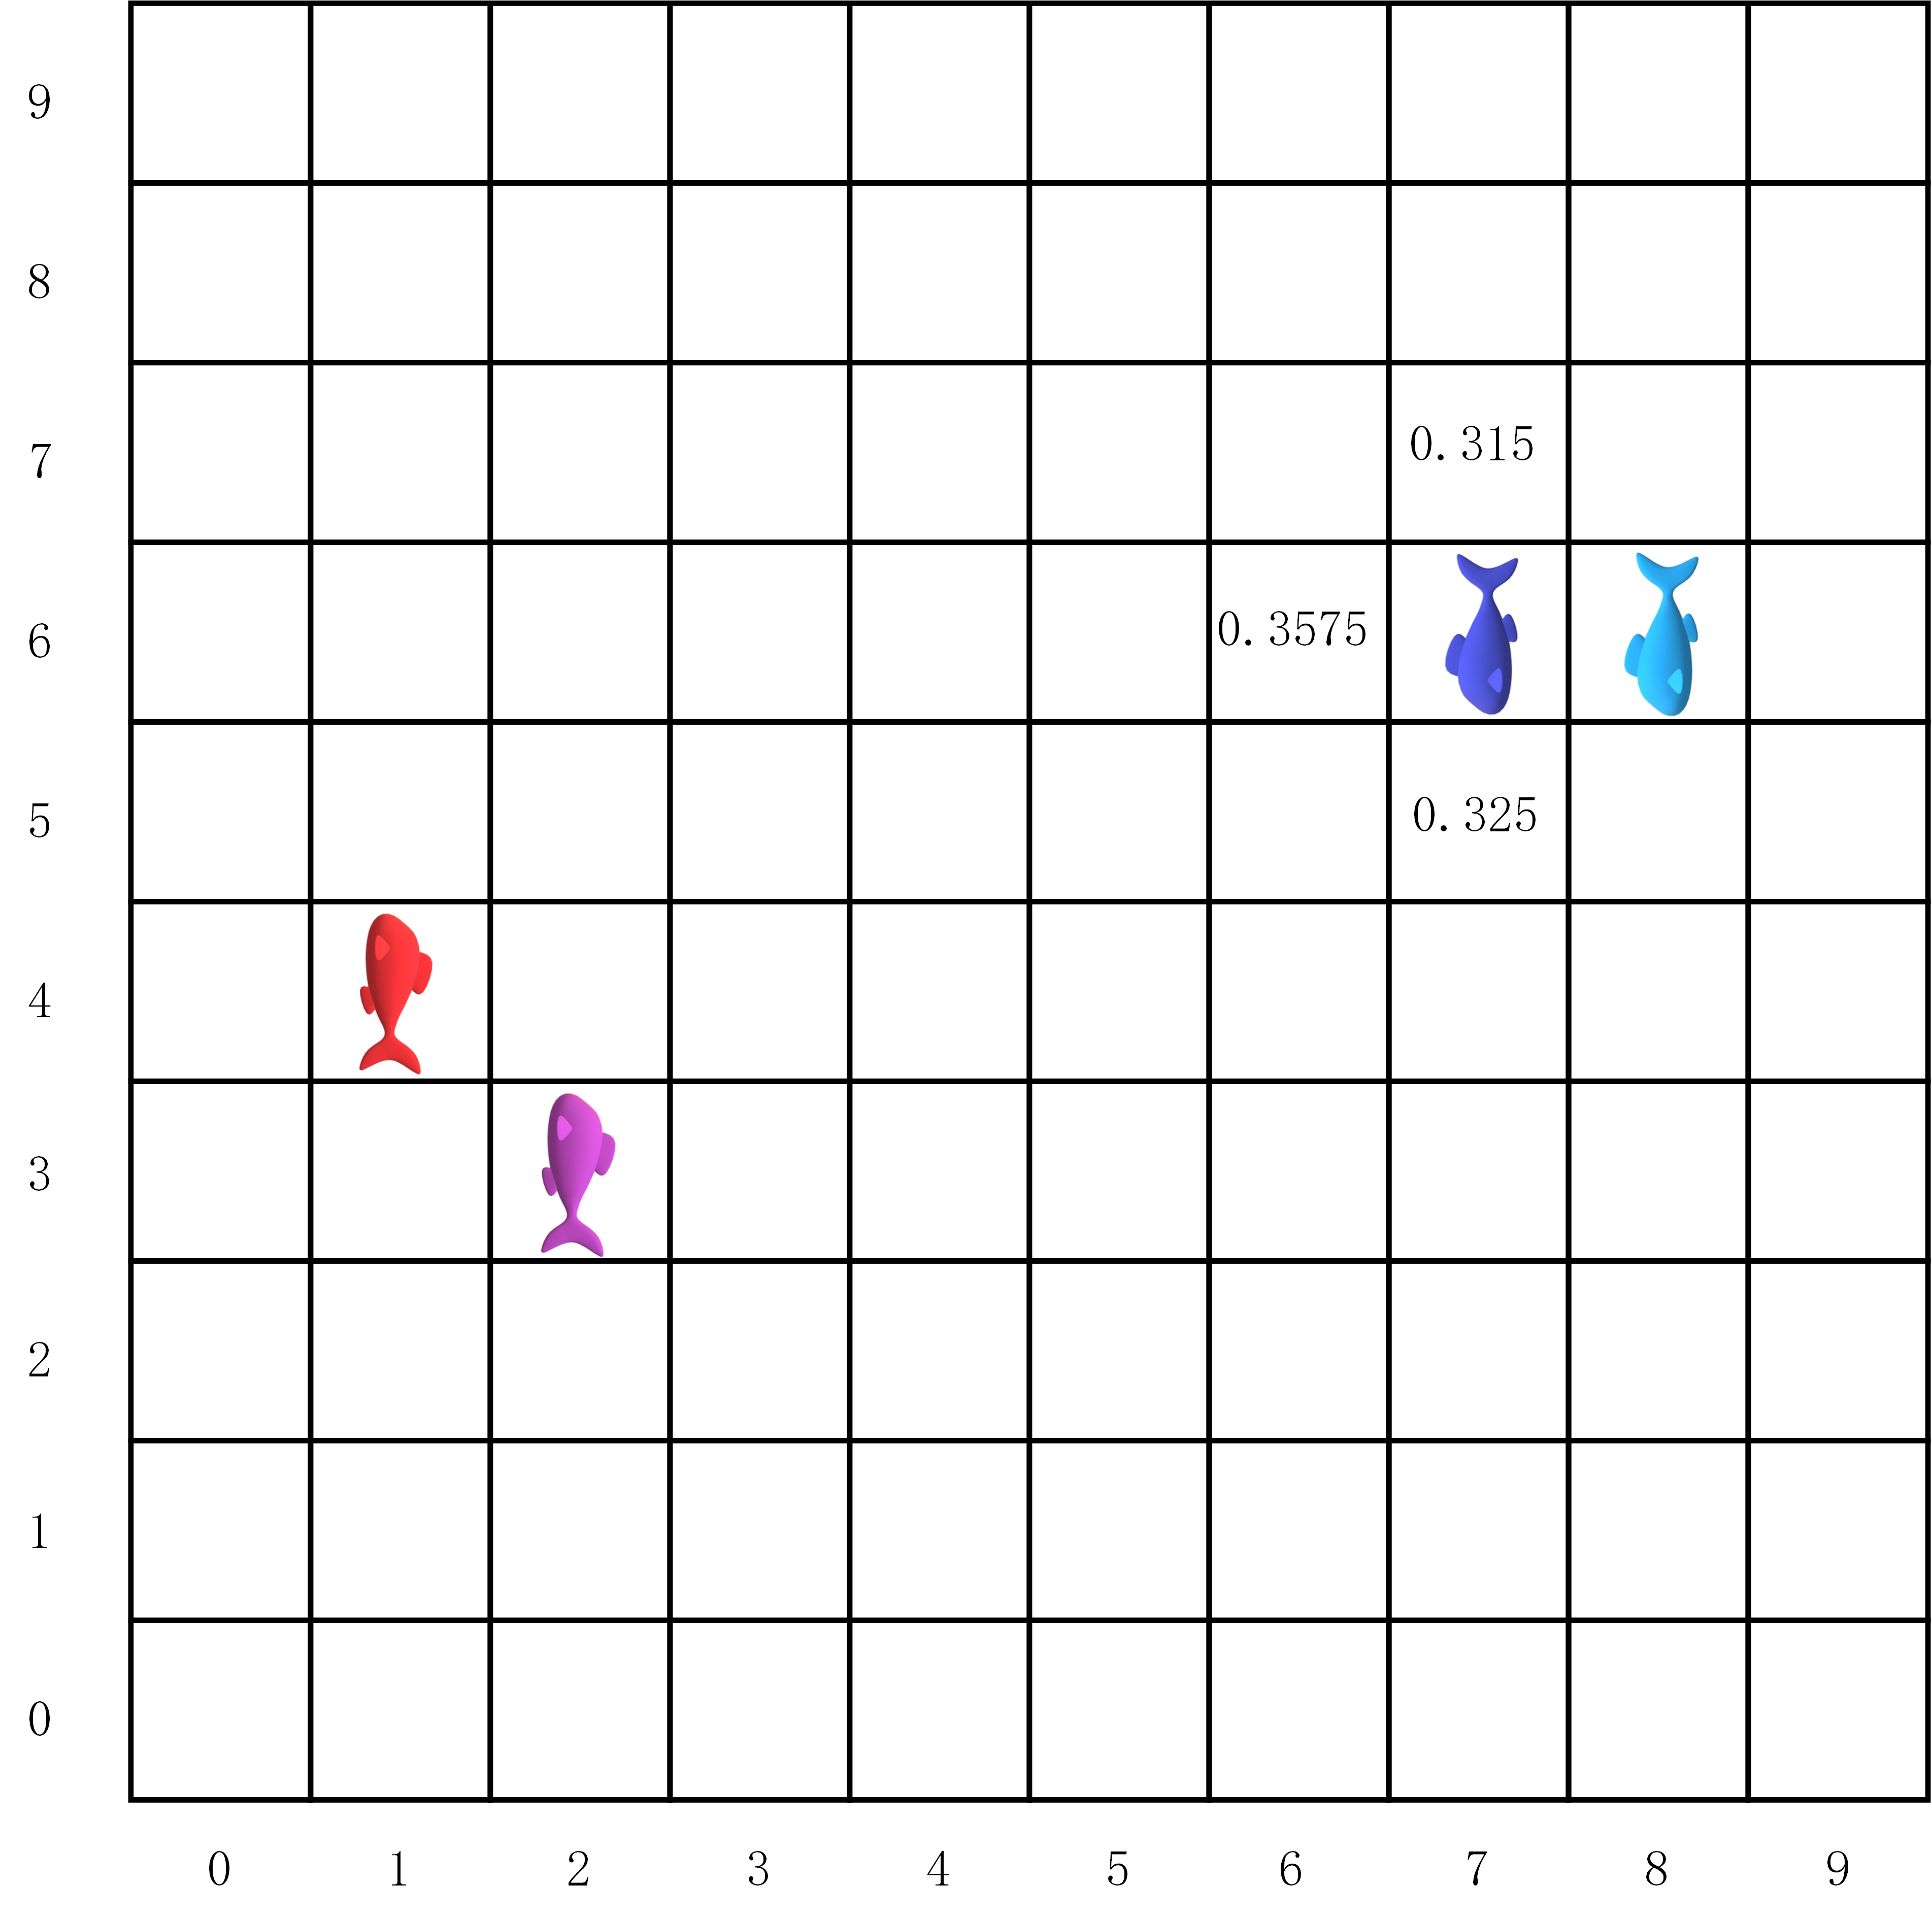
\includegraphics[width=10cm]{example/duoduiduo2.jpg}
	\bicaption[这里将出现在插图索引]
	{蓝方起始状态信息}
	{Neural network training pipeline}
	\label{duoduiduo2.png}
\end{figure}
模型在test过程用贪心策略,选择概率最大的动作向左走,然后人类控制粉色小鱼向右,通过搜索算法统计得到浅蓝色小鱼的策略如图:

\begin{figure}[!htp]
	\centering
	\subcaptionbox{\label{fig2:fig:duoduiduo3-6:a}}
	{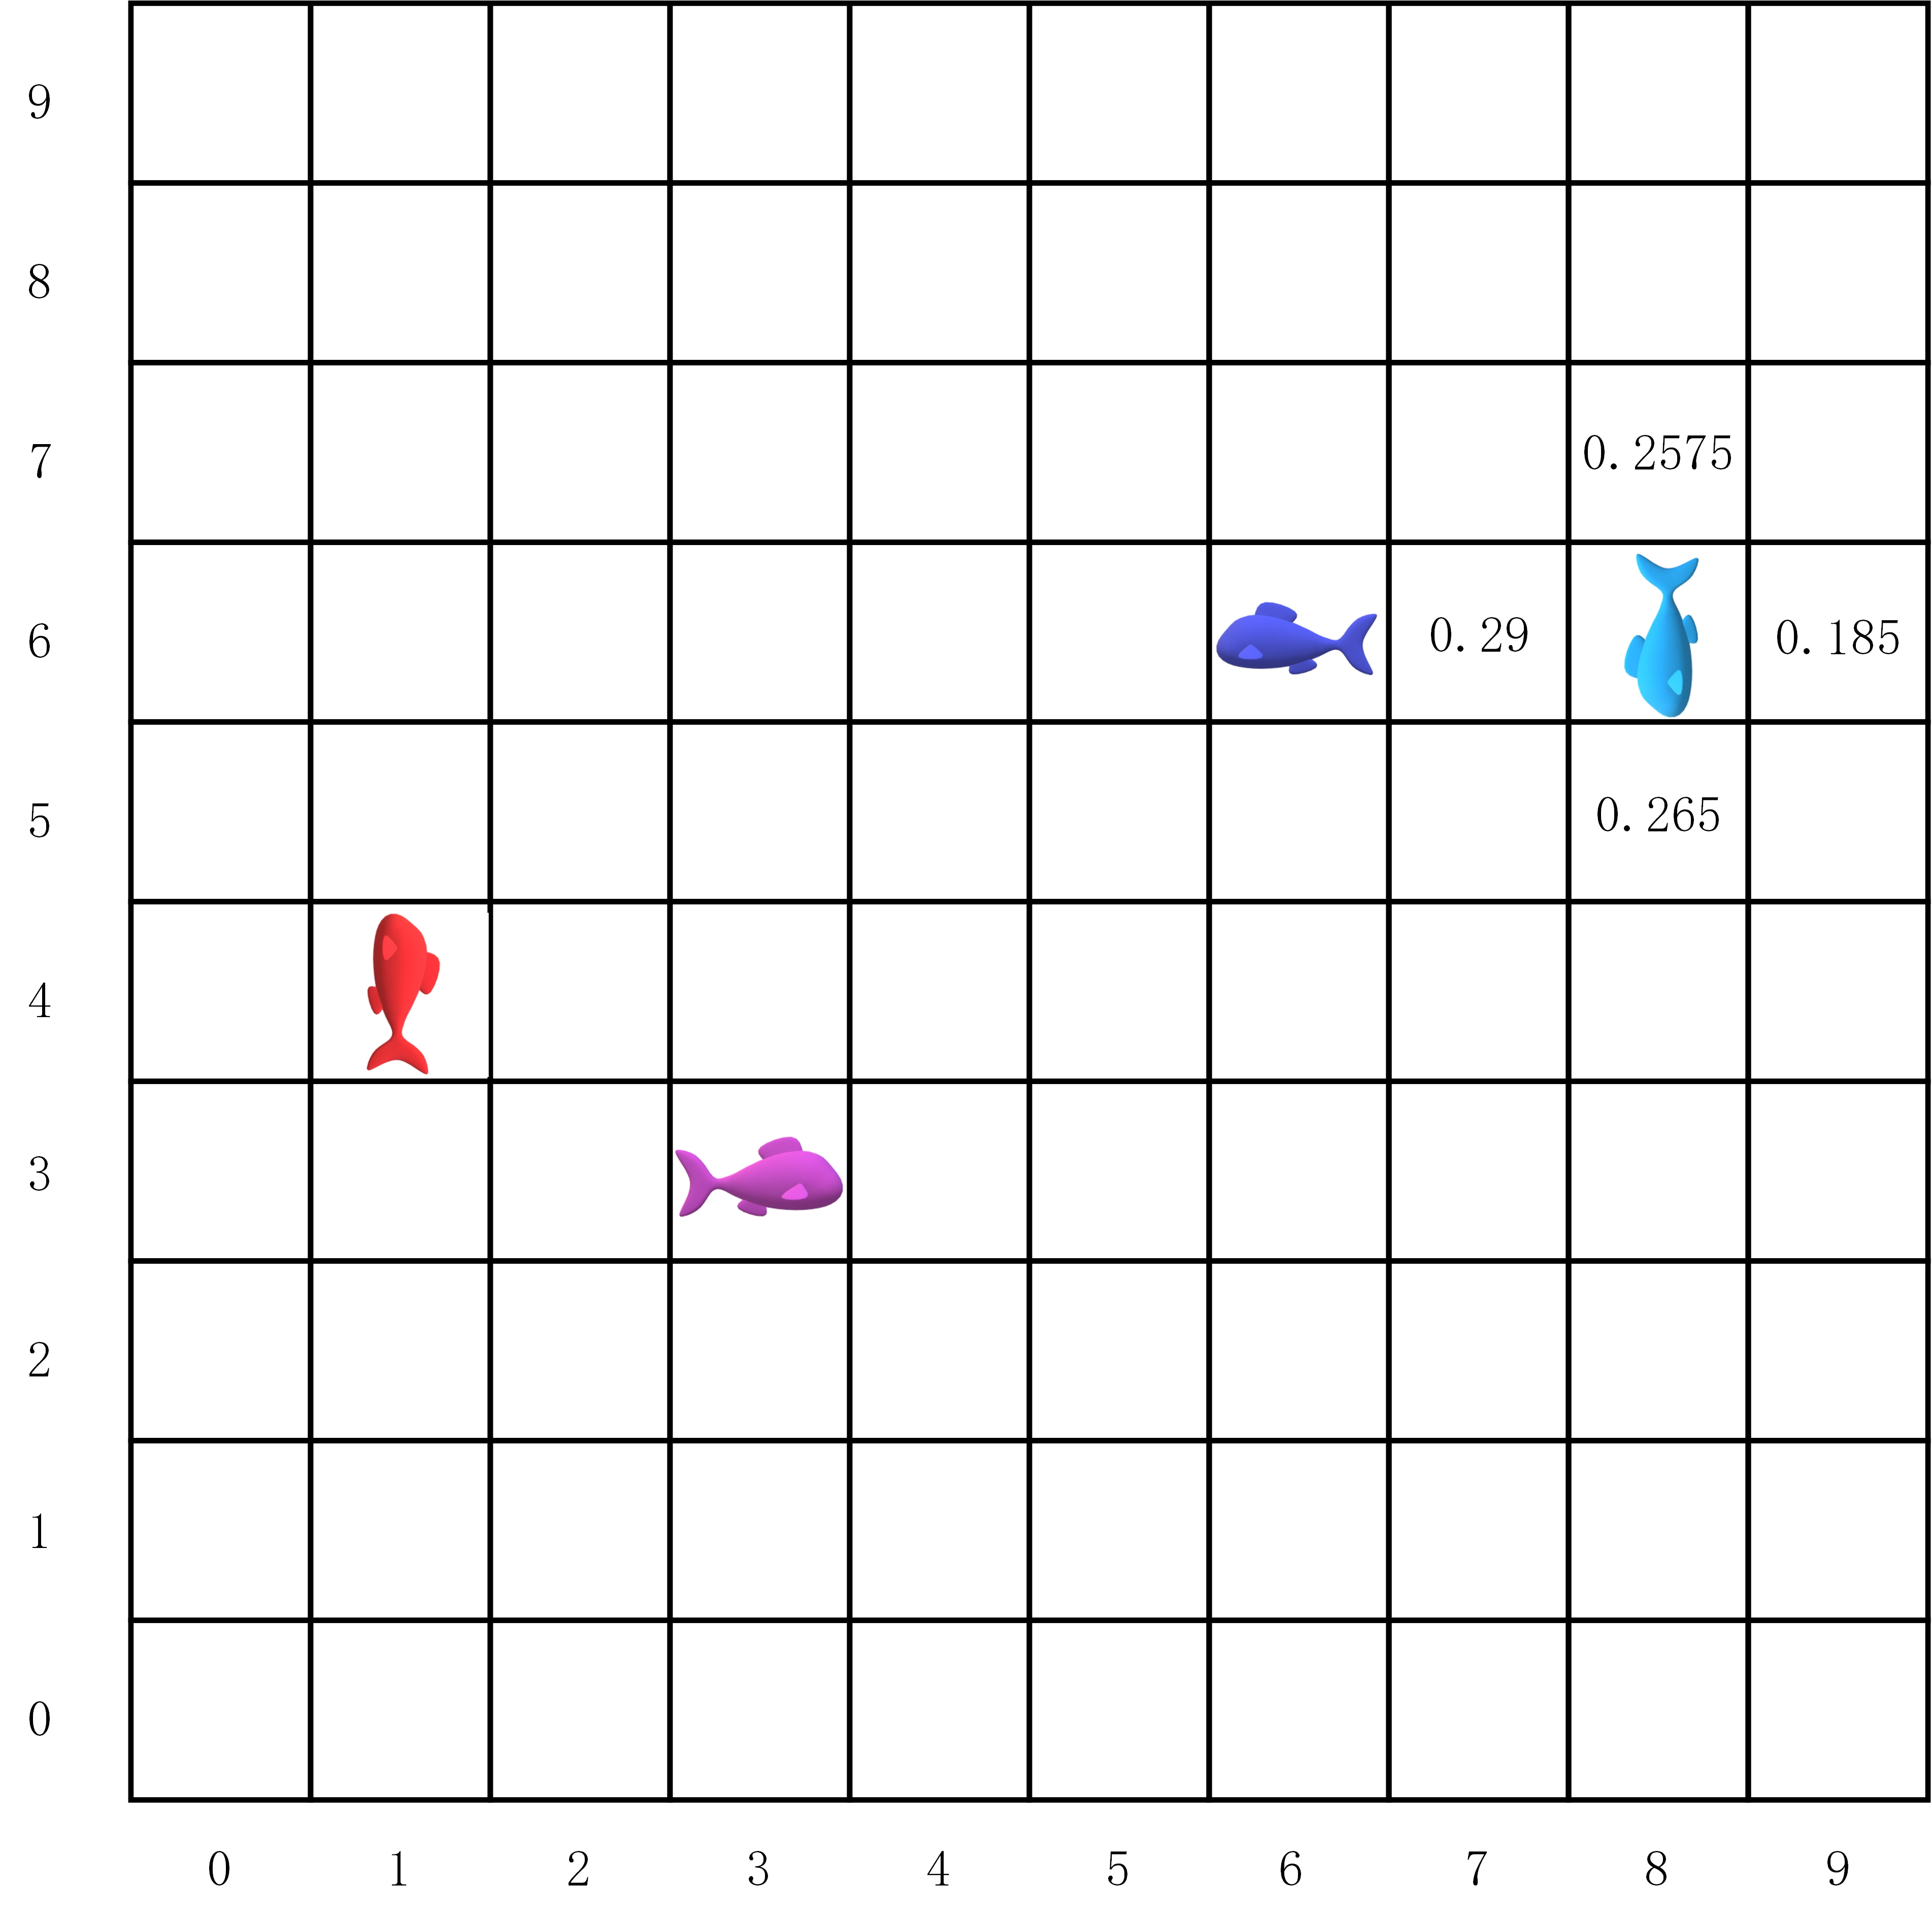
\includegraphics[width=0.45\hsize,height=0.45\hsize]{example/duoduiduo3.jpg}}
	\hspace{0.5em}
	\subcaptionbox{\label{fig:duoduiduo3-6:b}}
	{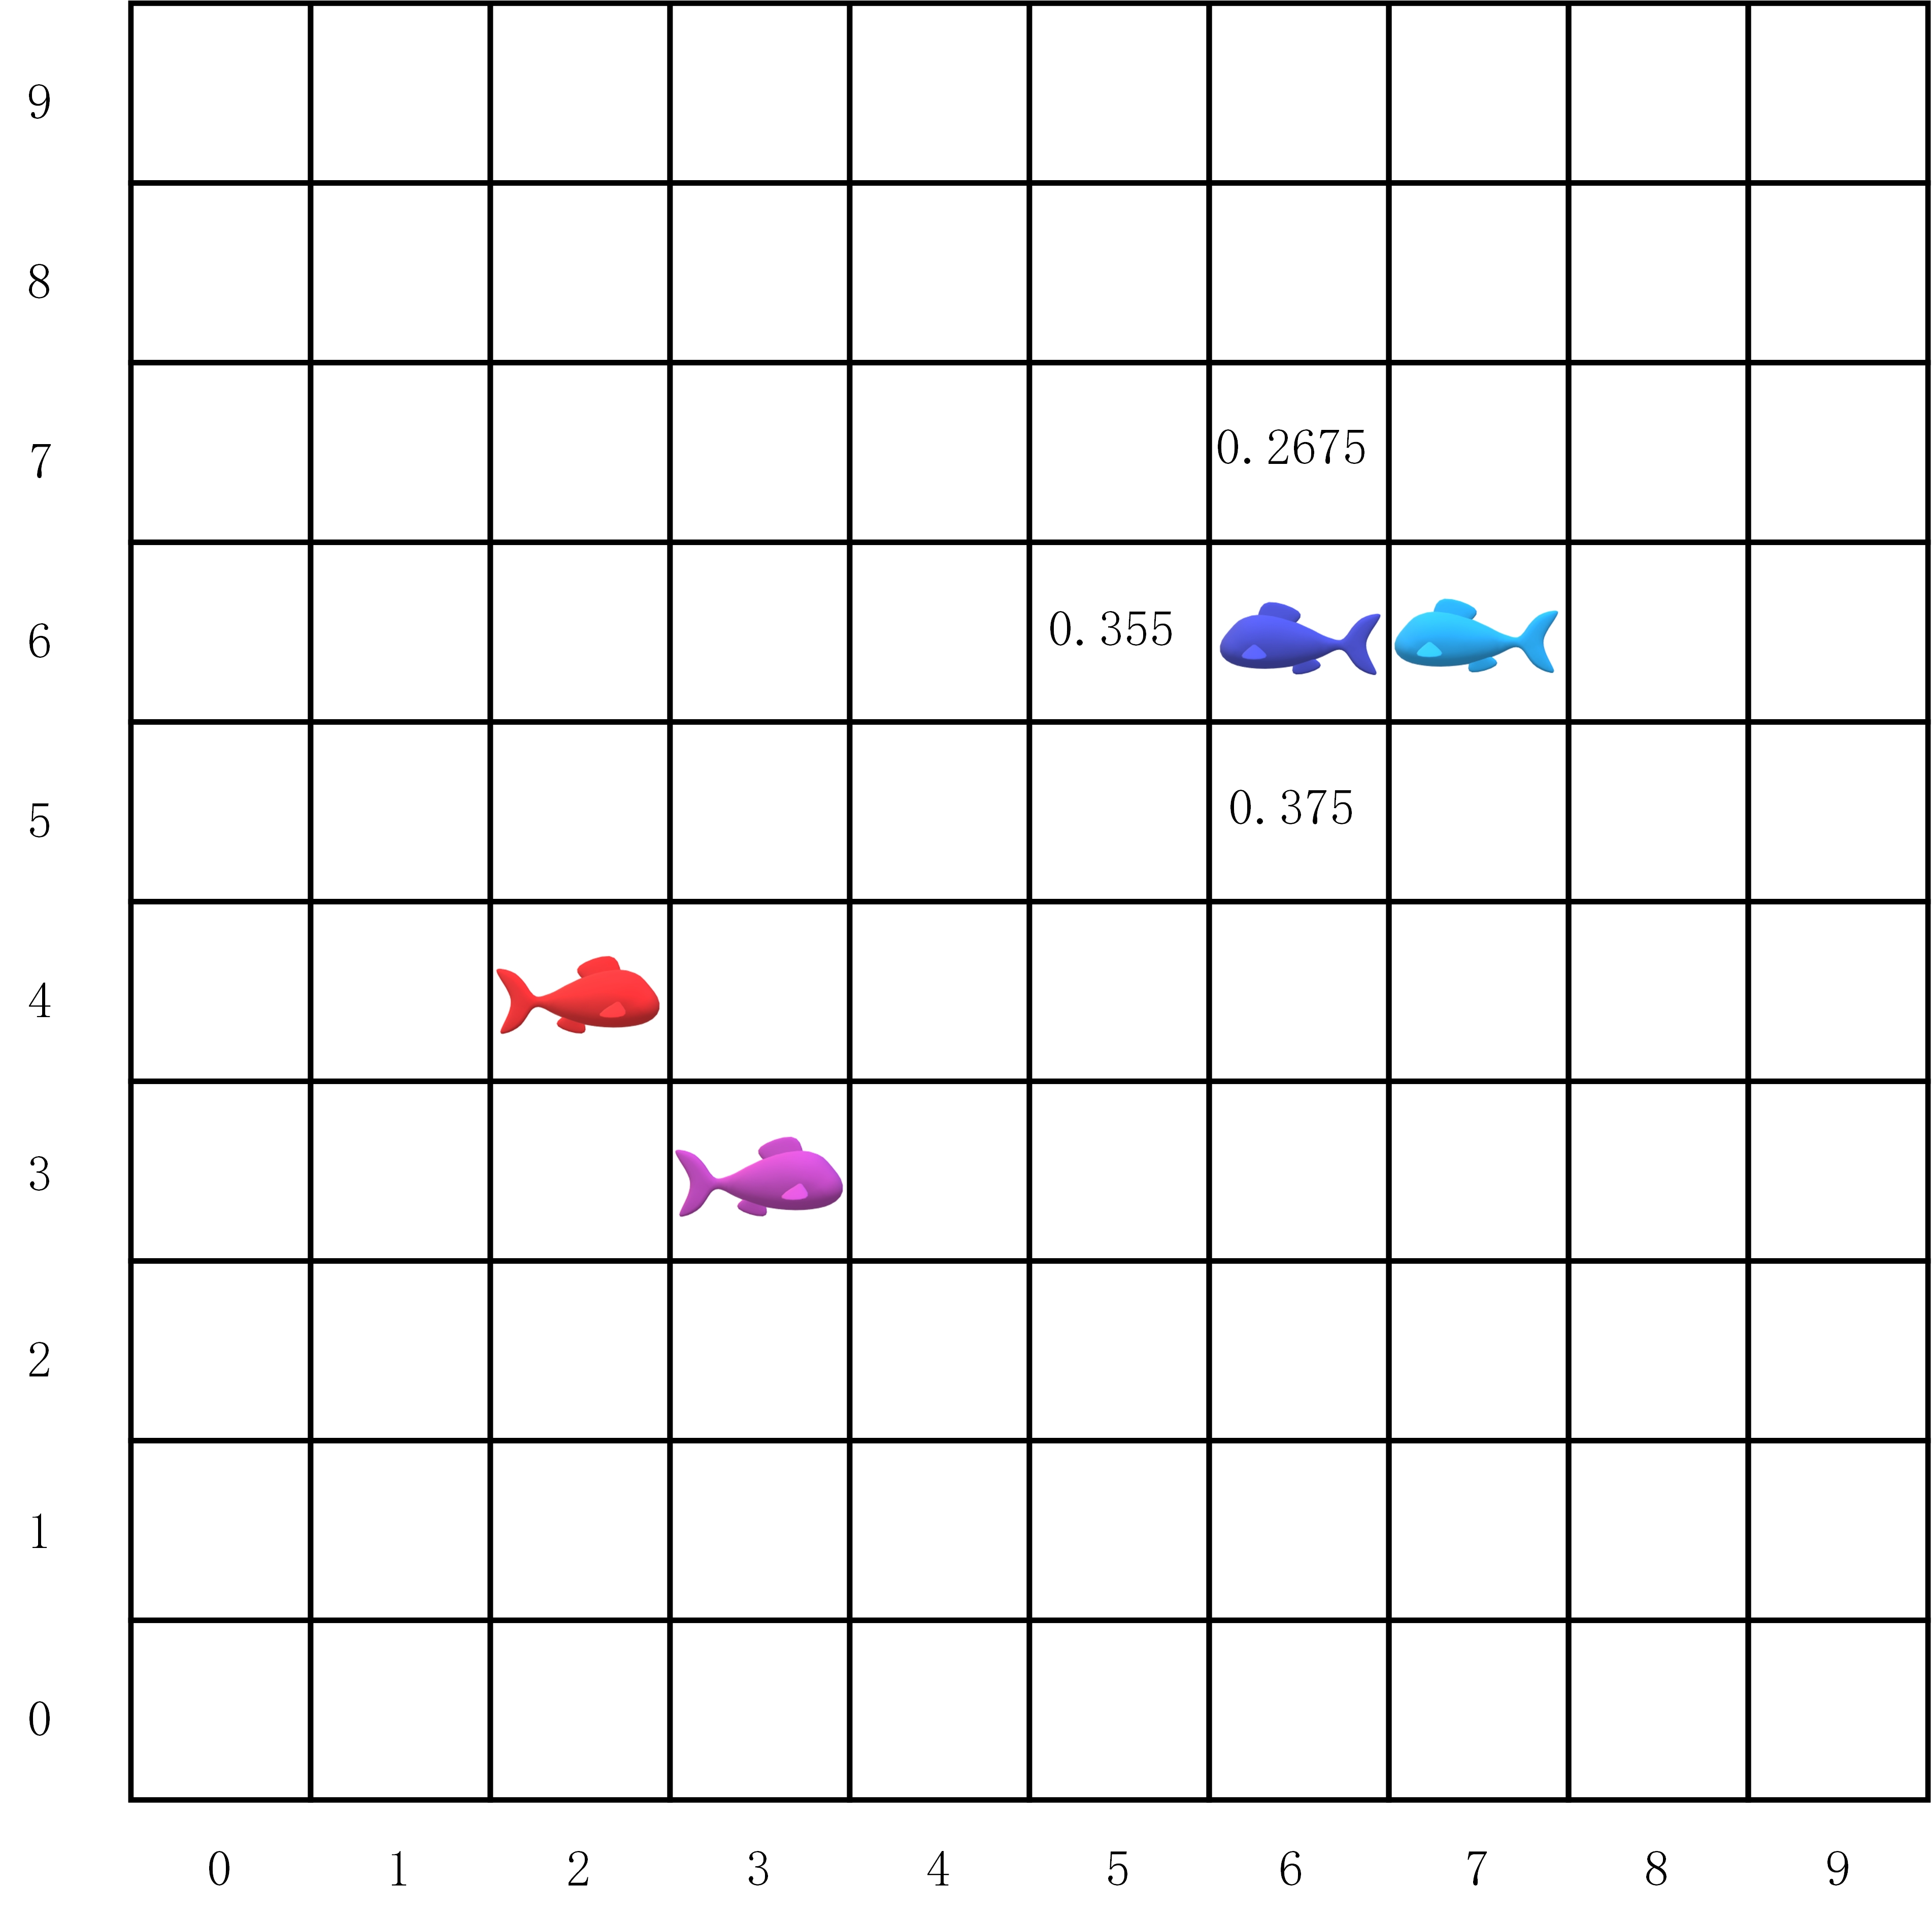
\includegraphics[width=0.45\hsize,height=0.45\hsize]{example/duoduiduo4.jpg}}
	\newline
	\centering
	\subcaptionbox{\label{fig:duoduiduo3-6:c}}
	{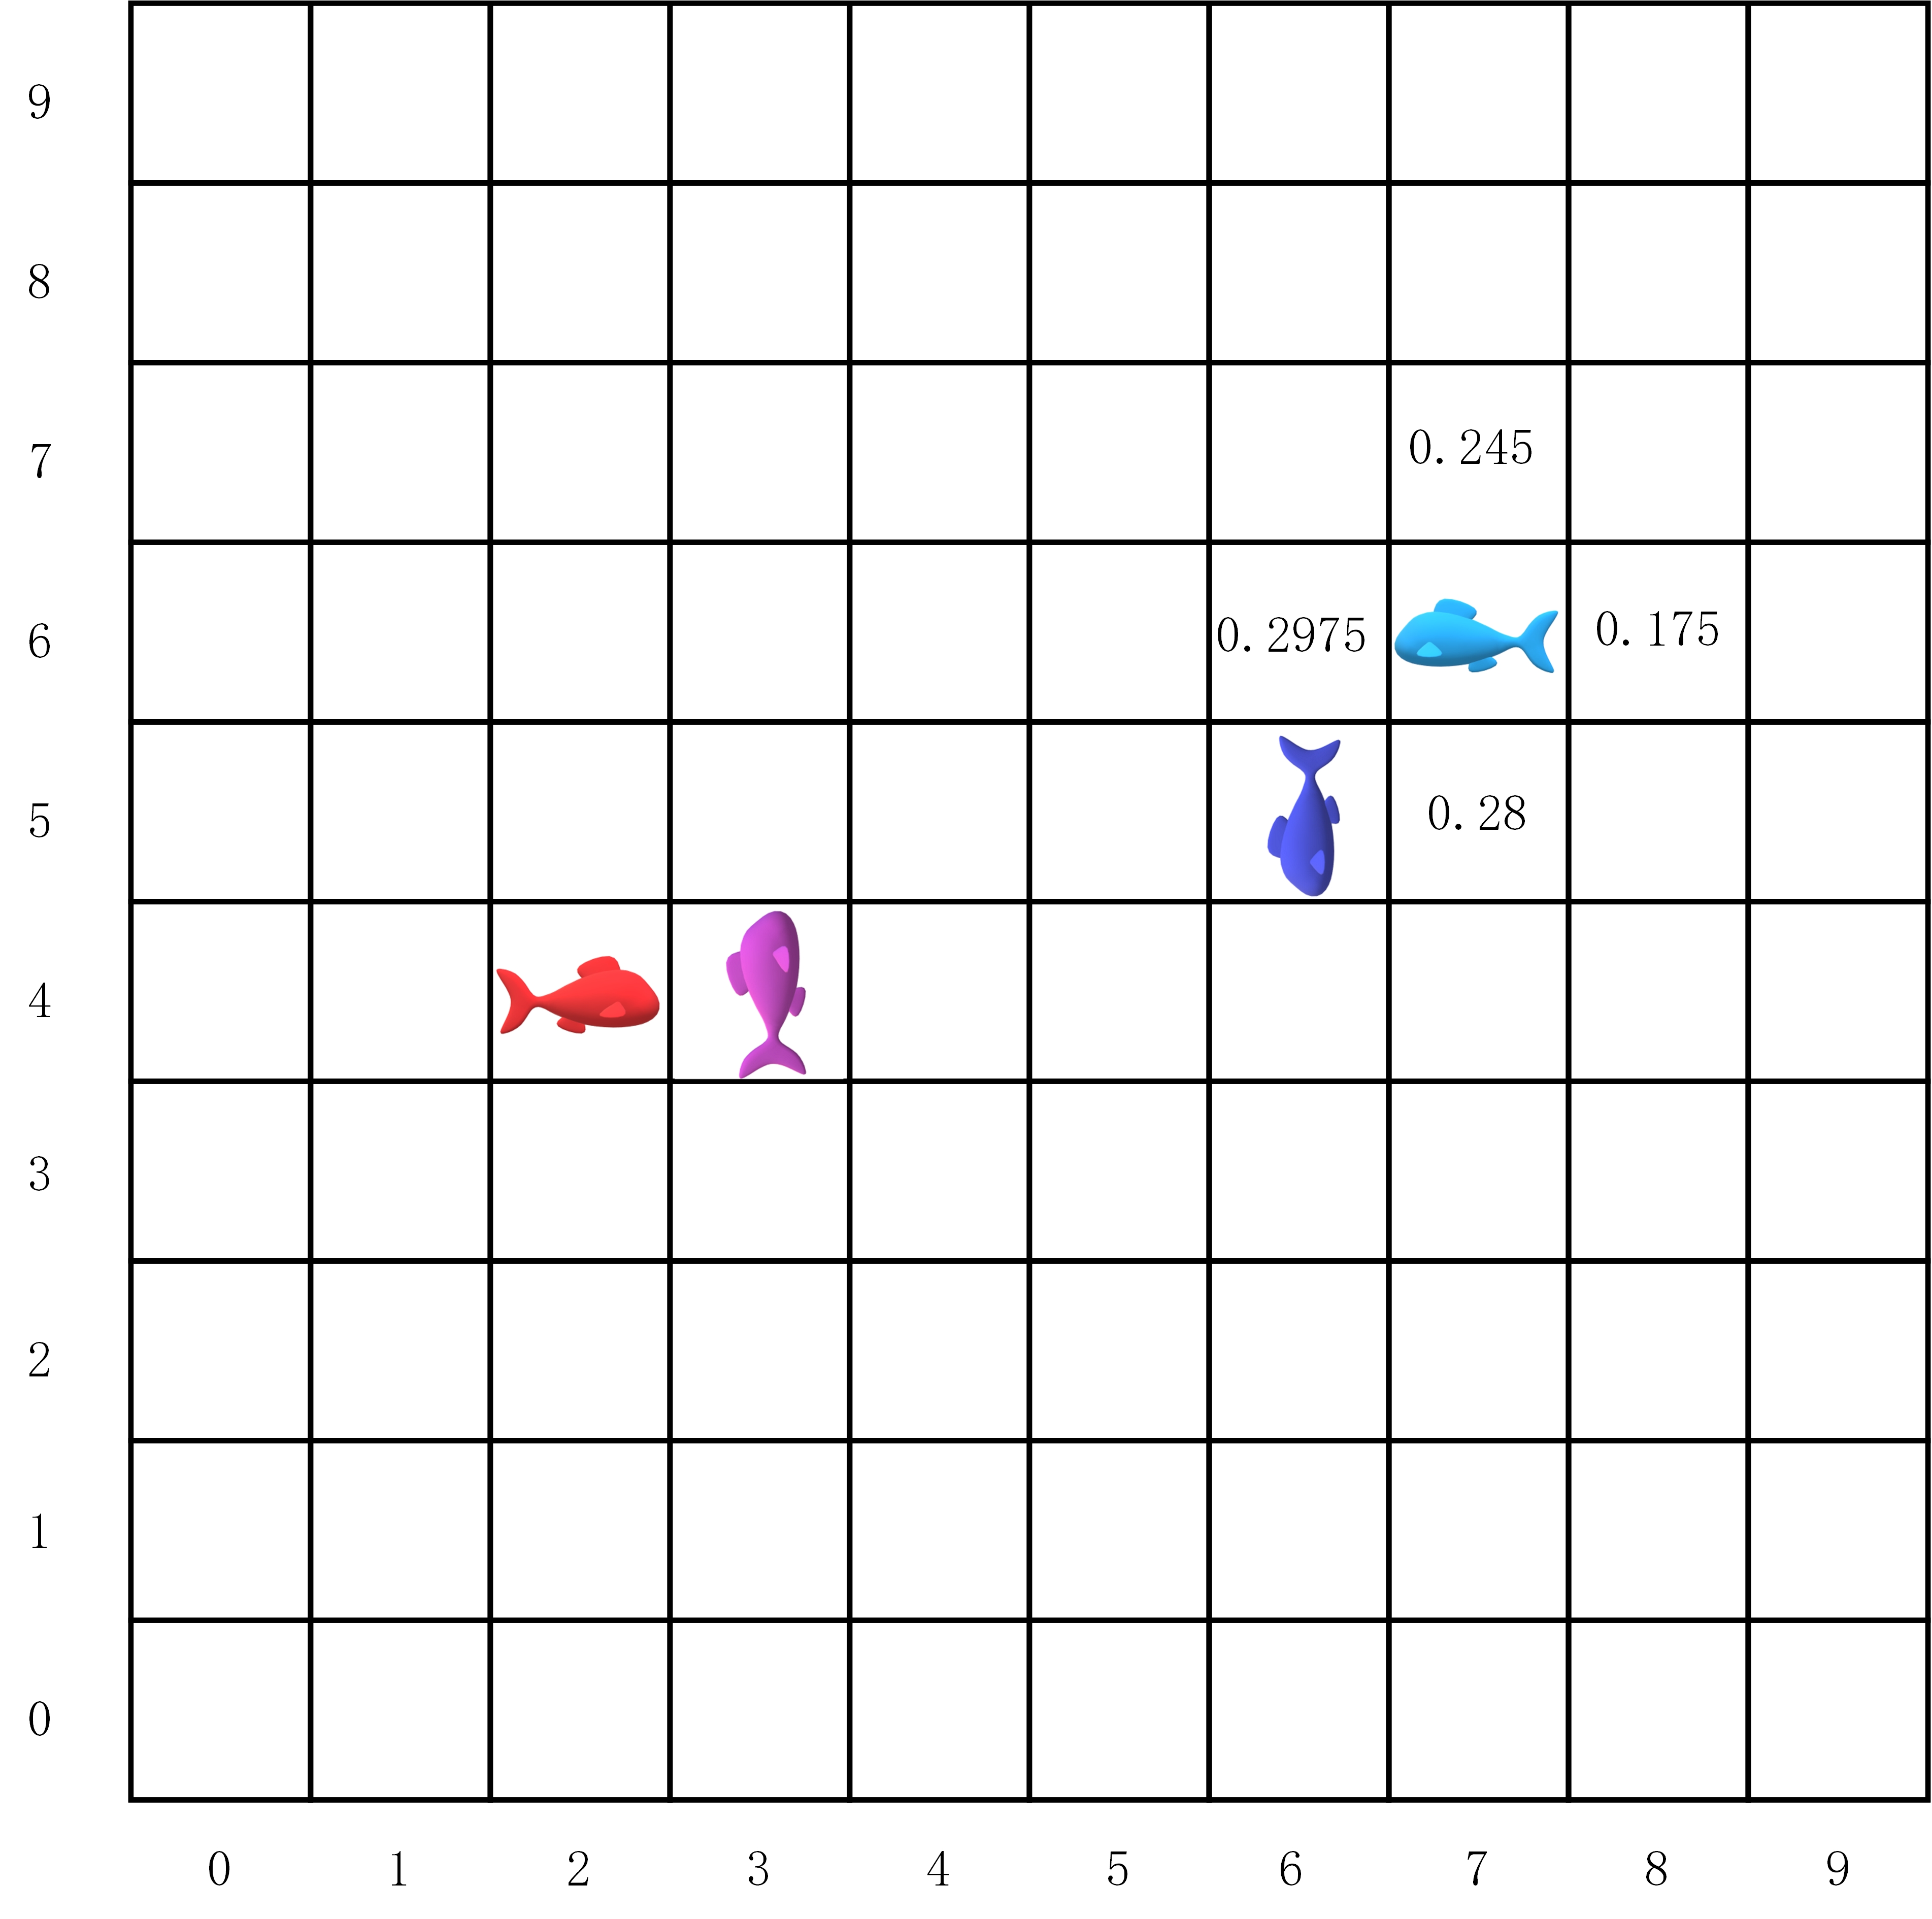
\includegraphics[width=0.45\hsize,height=0.45\hsize]{example/duoduiduo5.jpg}}
	\hspace{0.5em}
	\subcaptionbox{\label{fig:duoduiduo3-6:d}}
	{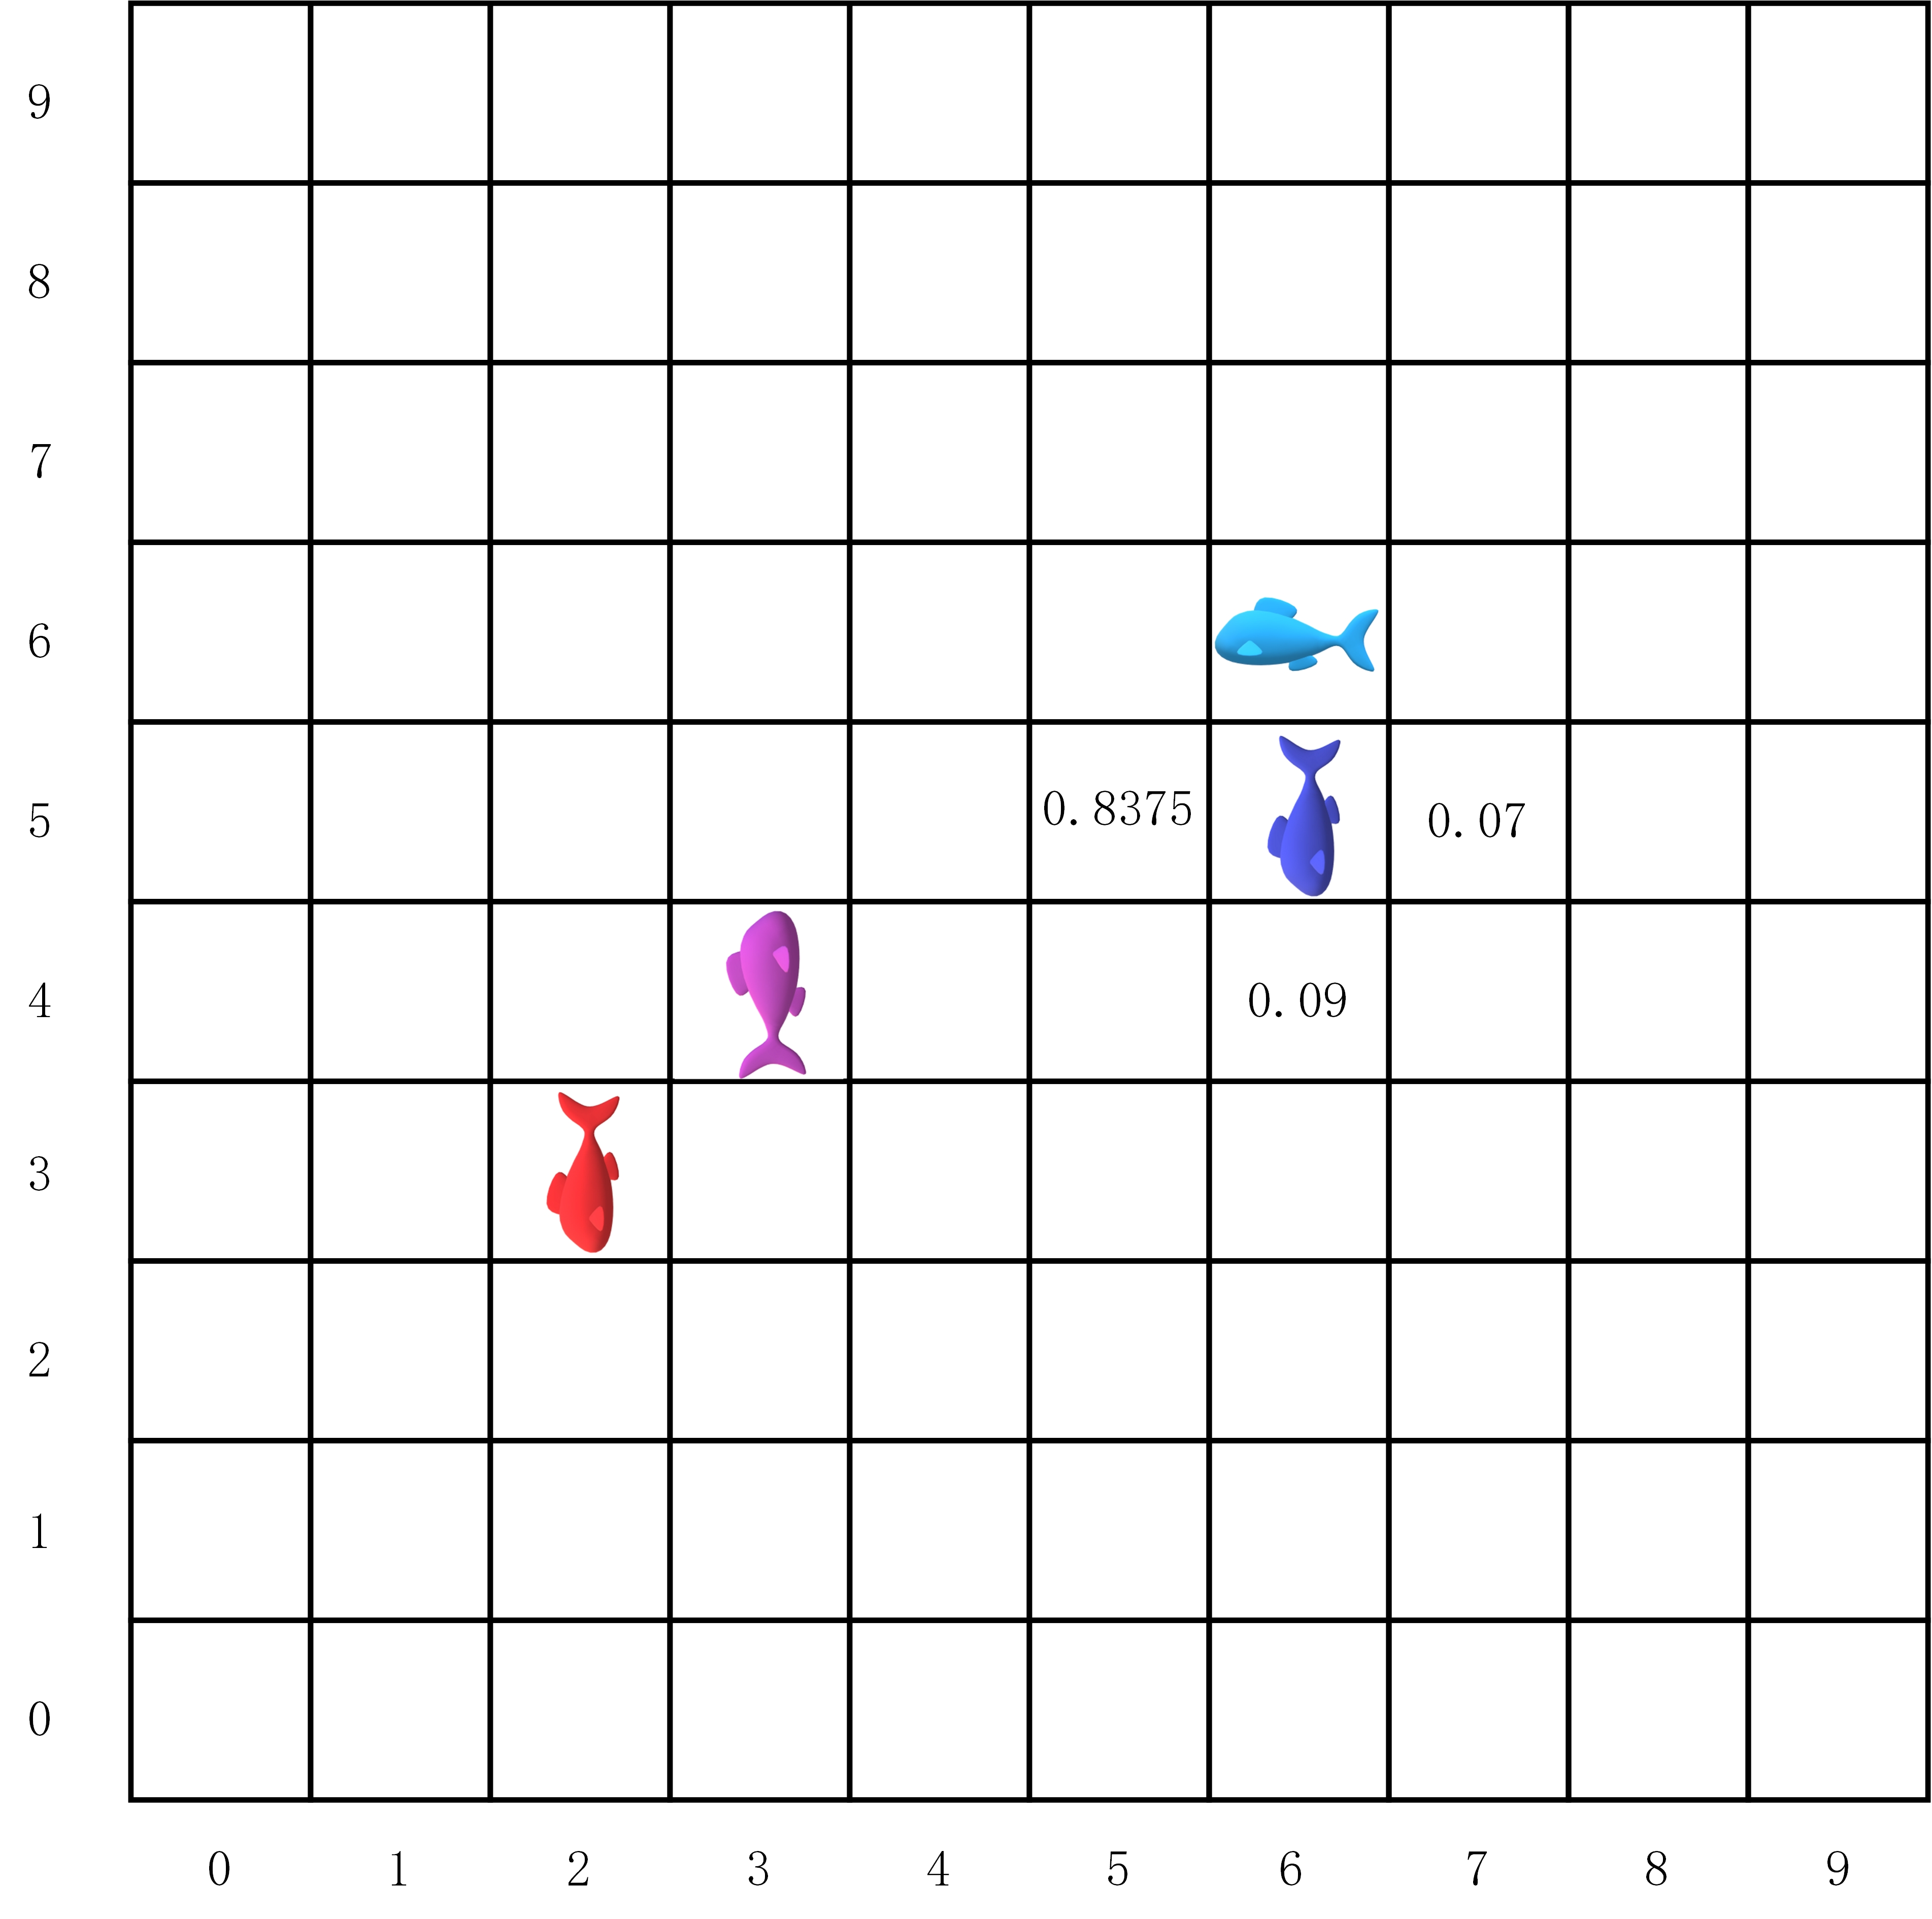
\includegraphics[width=0.45\hsize,height=0.45\hsize]{example/duoduiduo6.jpg}}
	\bicaption
	{多对多人机对弈过程图示}
	{Examples of response maps during occlusions and not.The first row shows the original and response maps with no occlusions while the second row shows the maps with occlusions. The first column are the shots of sequence bear front in Princeton dataset. The color response maps are in the second column while the depth’s are in the third.}
	\label{fig:duoduiduo3-6}
\end{figure}

经过以上的对战到达状态如图\ref{fig:duoduiduo3-6:d},可以看出这时对于深蓝色小鱼的策略已经非常明确,模型以0.8375的概率让深蓝色小鱼向左移动。下面分析当深蓝色小鱼分别执行可行的左,下,右的情况。
当小鱼向下移动时,和对方智能体相对状态如图\ref{fig:duoduiduo9.jpg}


\begin{figure}[!hpbt]
	\centering
	\subcaptionbox{向下状态\label{fig2:duoduiduo:a}}
	{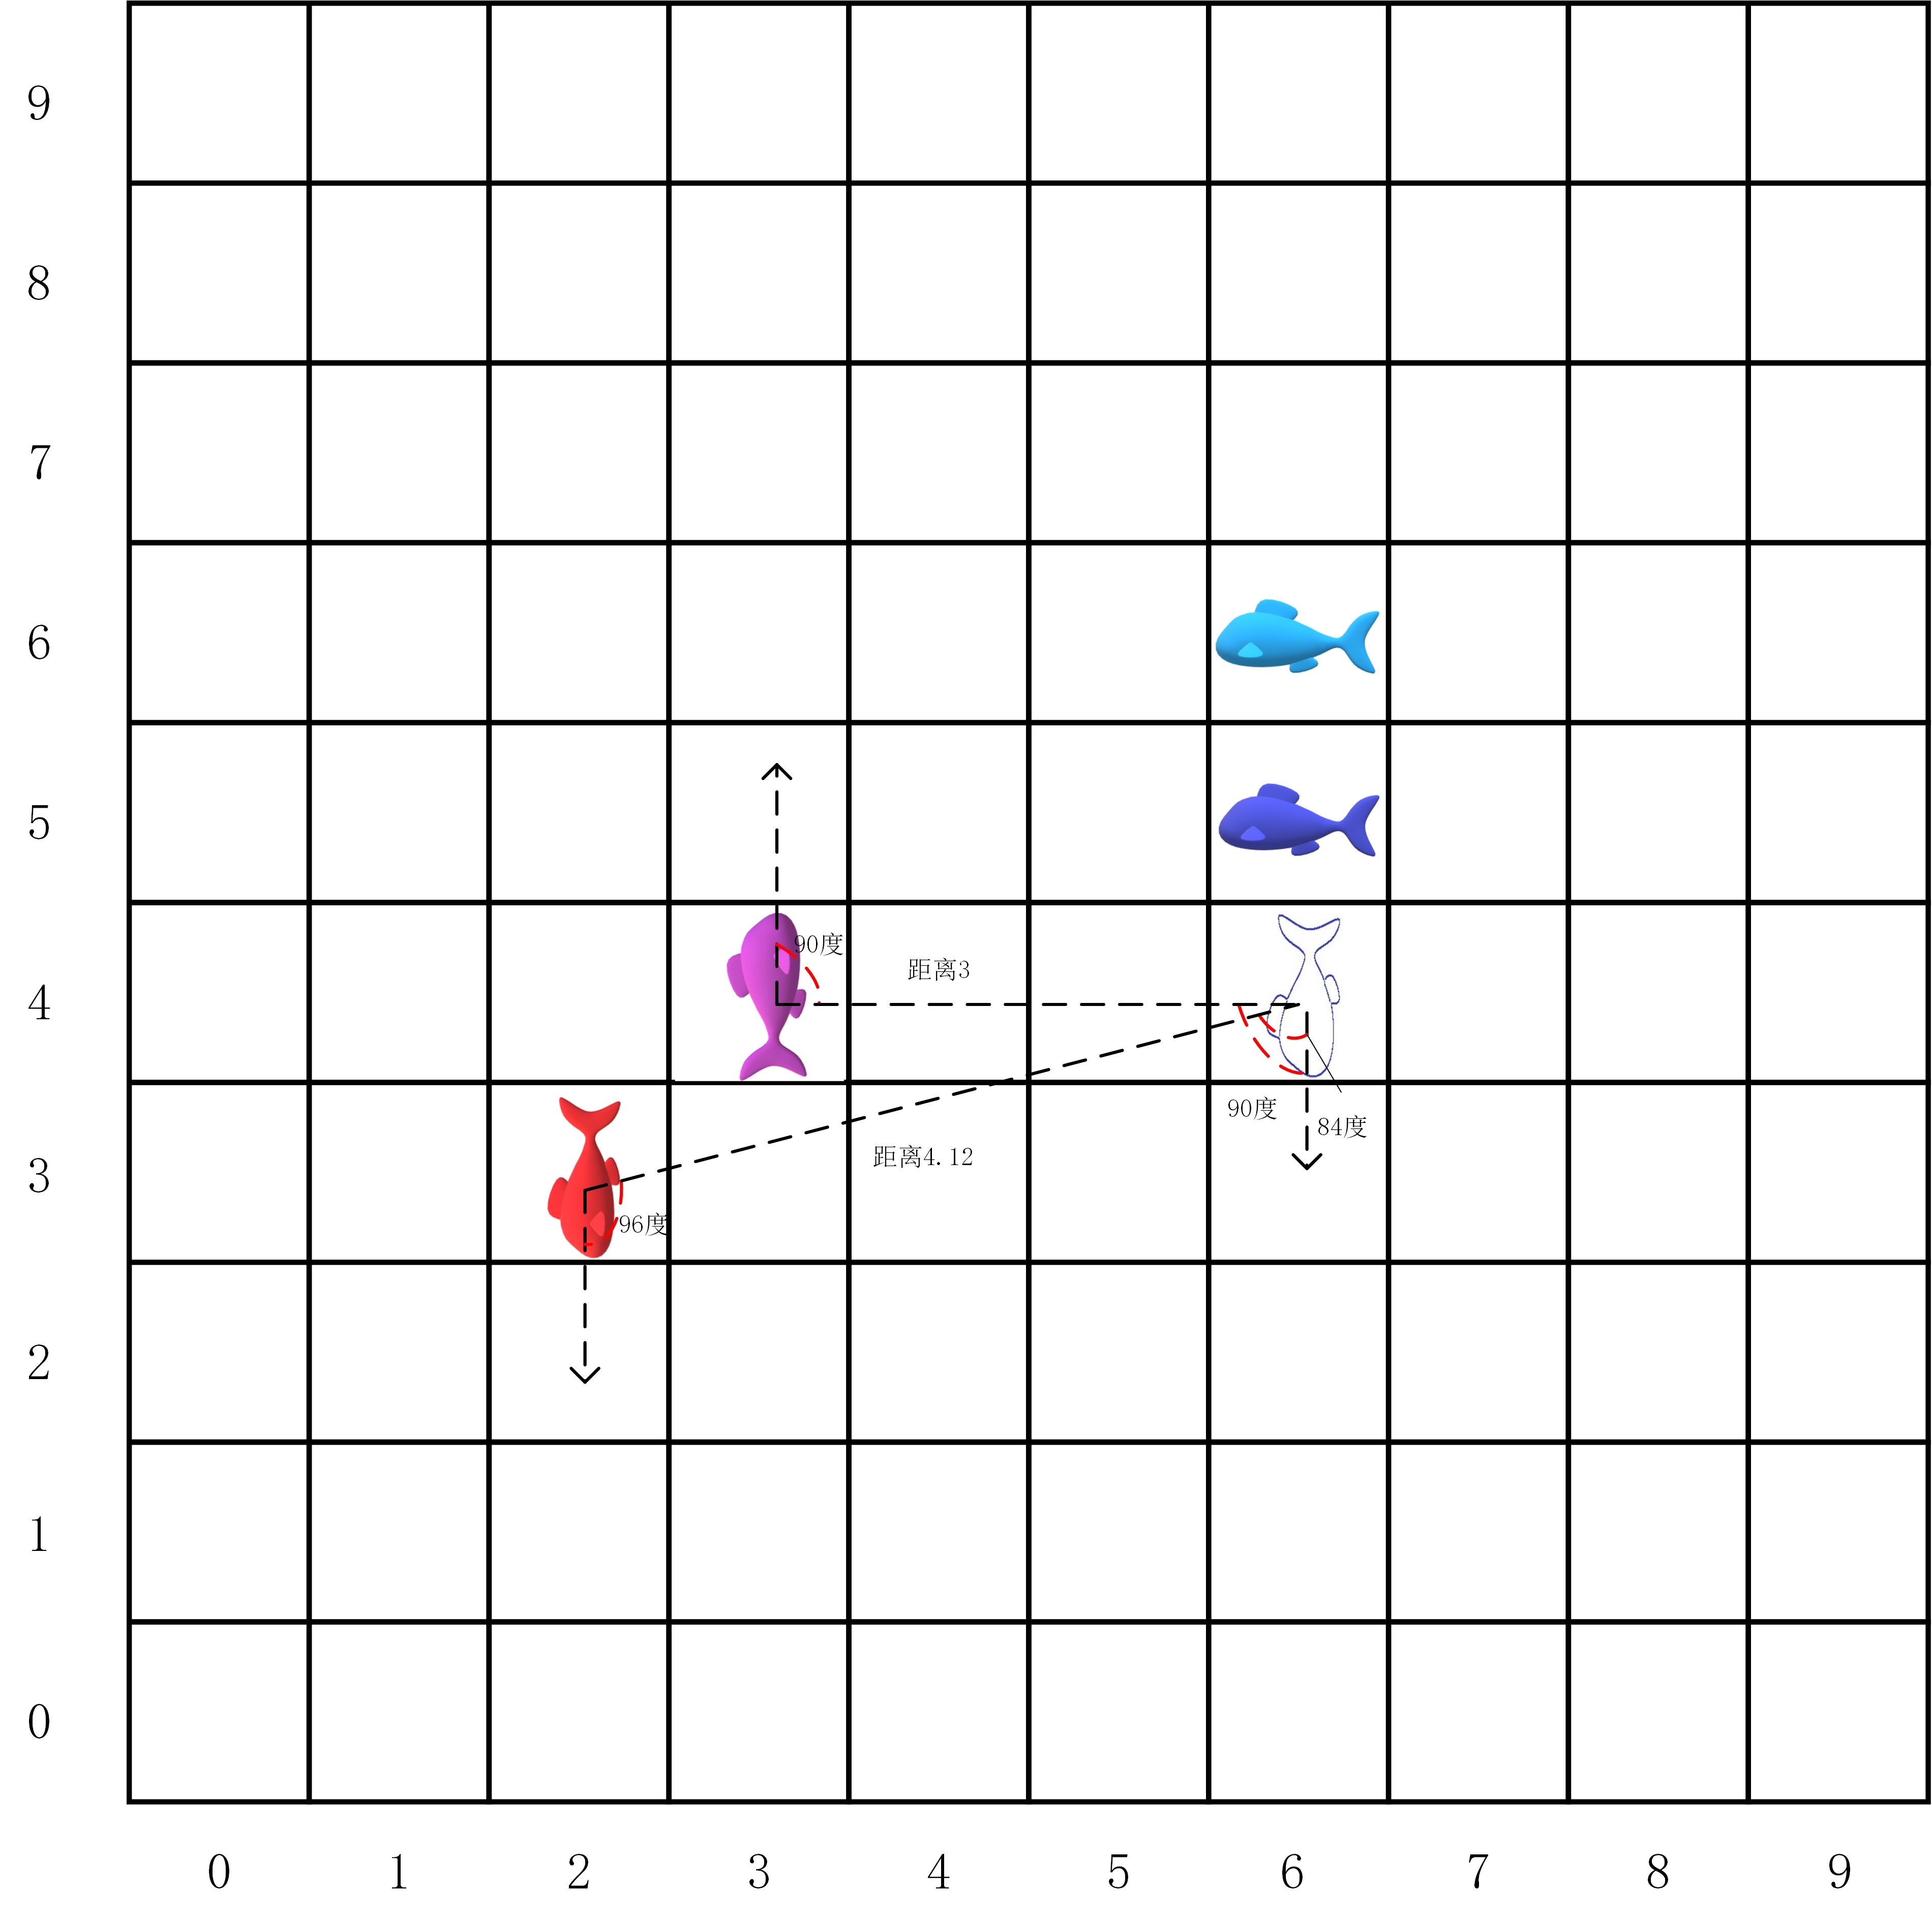
\includegraphics[width=0.45\hsize,height=0.45\hsize]{example/duoduiduo7.jpg}}
	\hspace{0.5em}
	\subcaptionbox{向右状态\label{fig2:duoduiduo:b}}
	{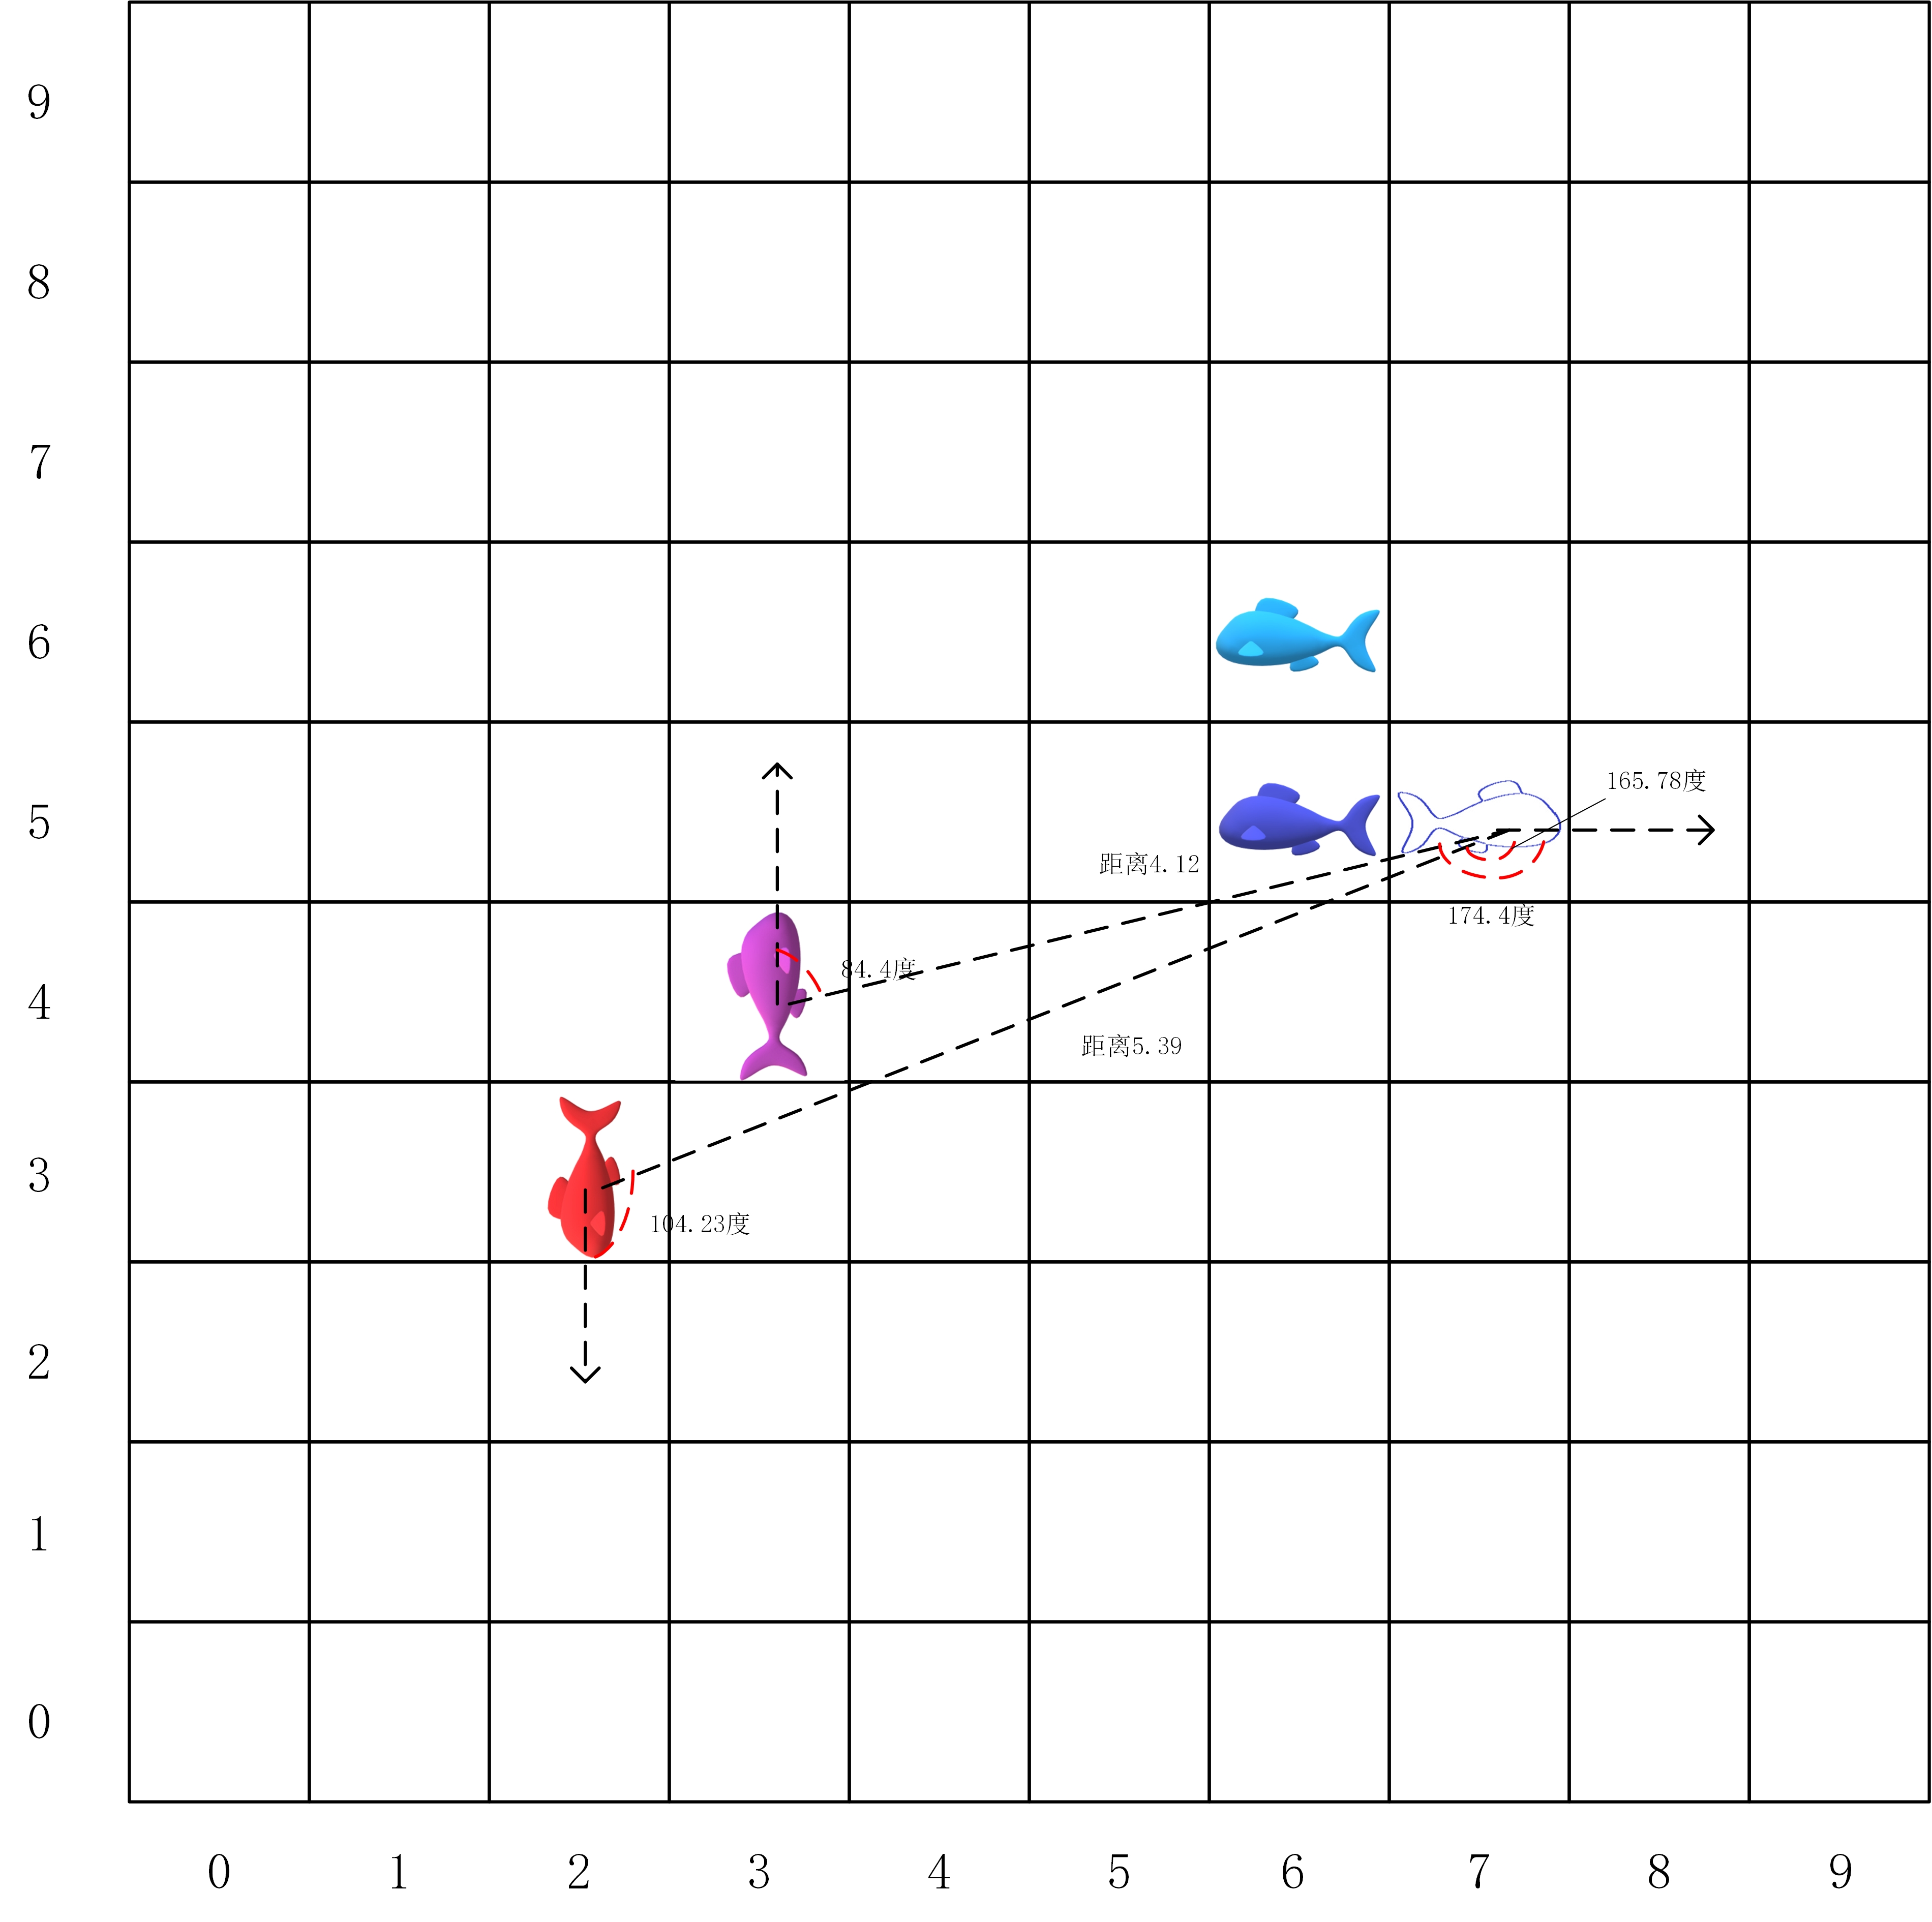
\includegraphics[width=0.45\hsize,height=0.45\hsize]{example/duoduiduo8.jpg}}
	\bicaption
	{多对多对弈状态分析}
	{Examples of response maps during occlusions and not.The first row shows the original and response maps with no occlusions while the second row shows the maps with occlusions. The first column are the shots of sequence bear front in Princeton dataset. The color response maps are in the second column while the depth’s are in the third.}
	\label{fig2:duoduiduo}
\end{figure}
经过计算蓝色小鱼向下移动和向右移动后与对方两个智能体相对状态,可以看出当向下和向右移动并不会吃掉对方小鱼,而当执行按照\ref{fig:duoduiduo3-6:d}策略,选取最大概率的动作向左时状态如图\ref{fig3:duoduiduo}
\begin{figure}[!hpbt]
	\centering
	\subcaptionbox{向左状态\label{fig3:duoduiduo:a}}
	{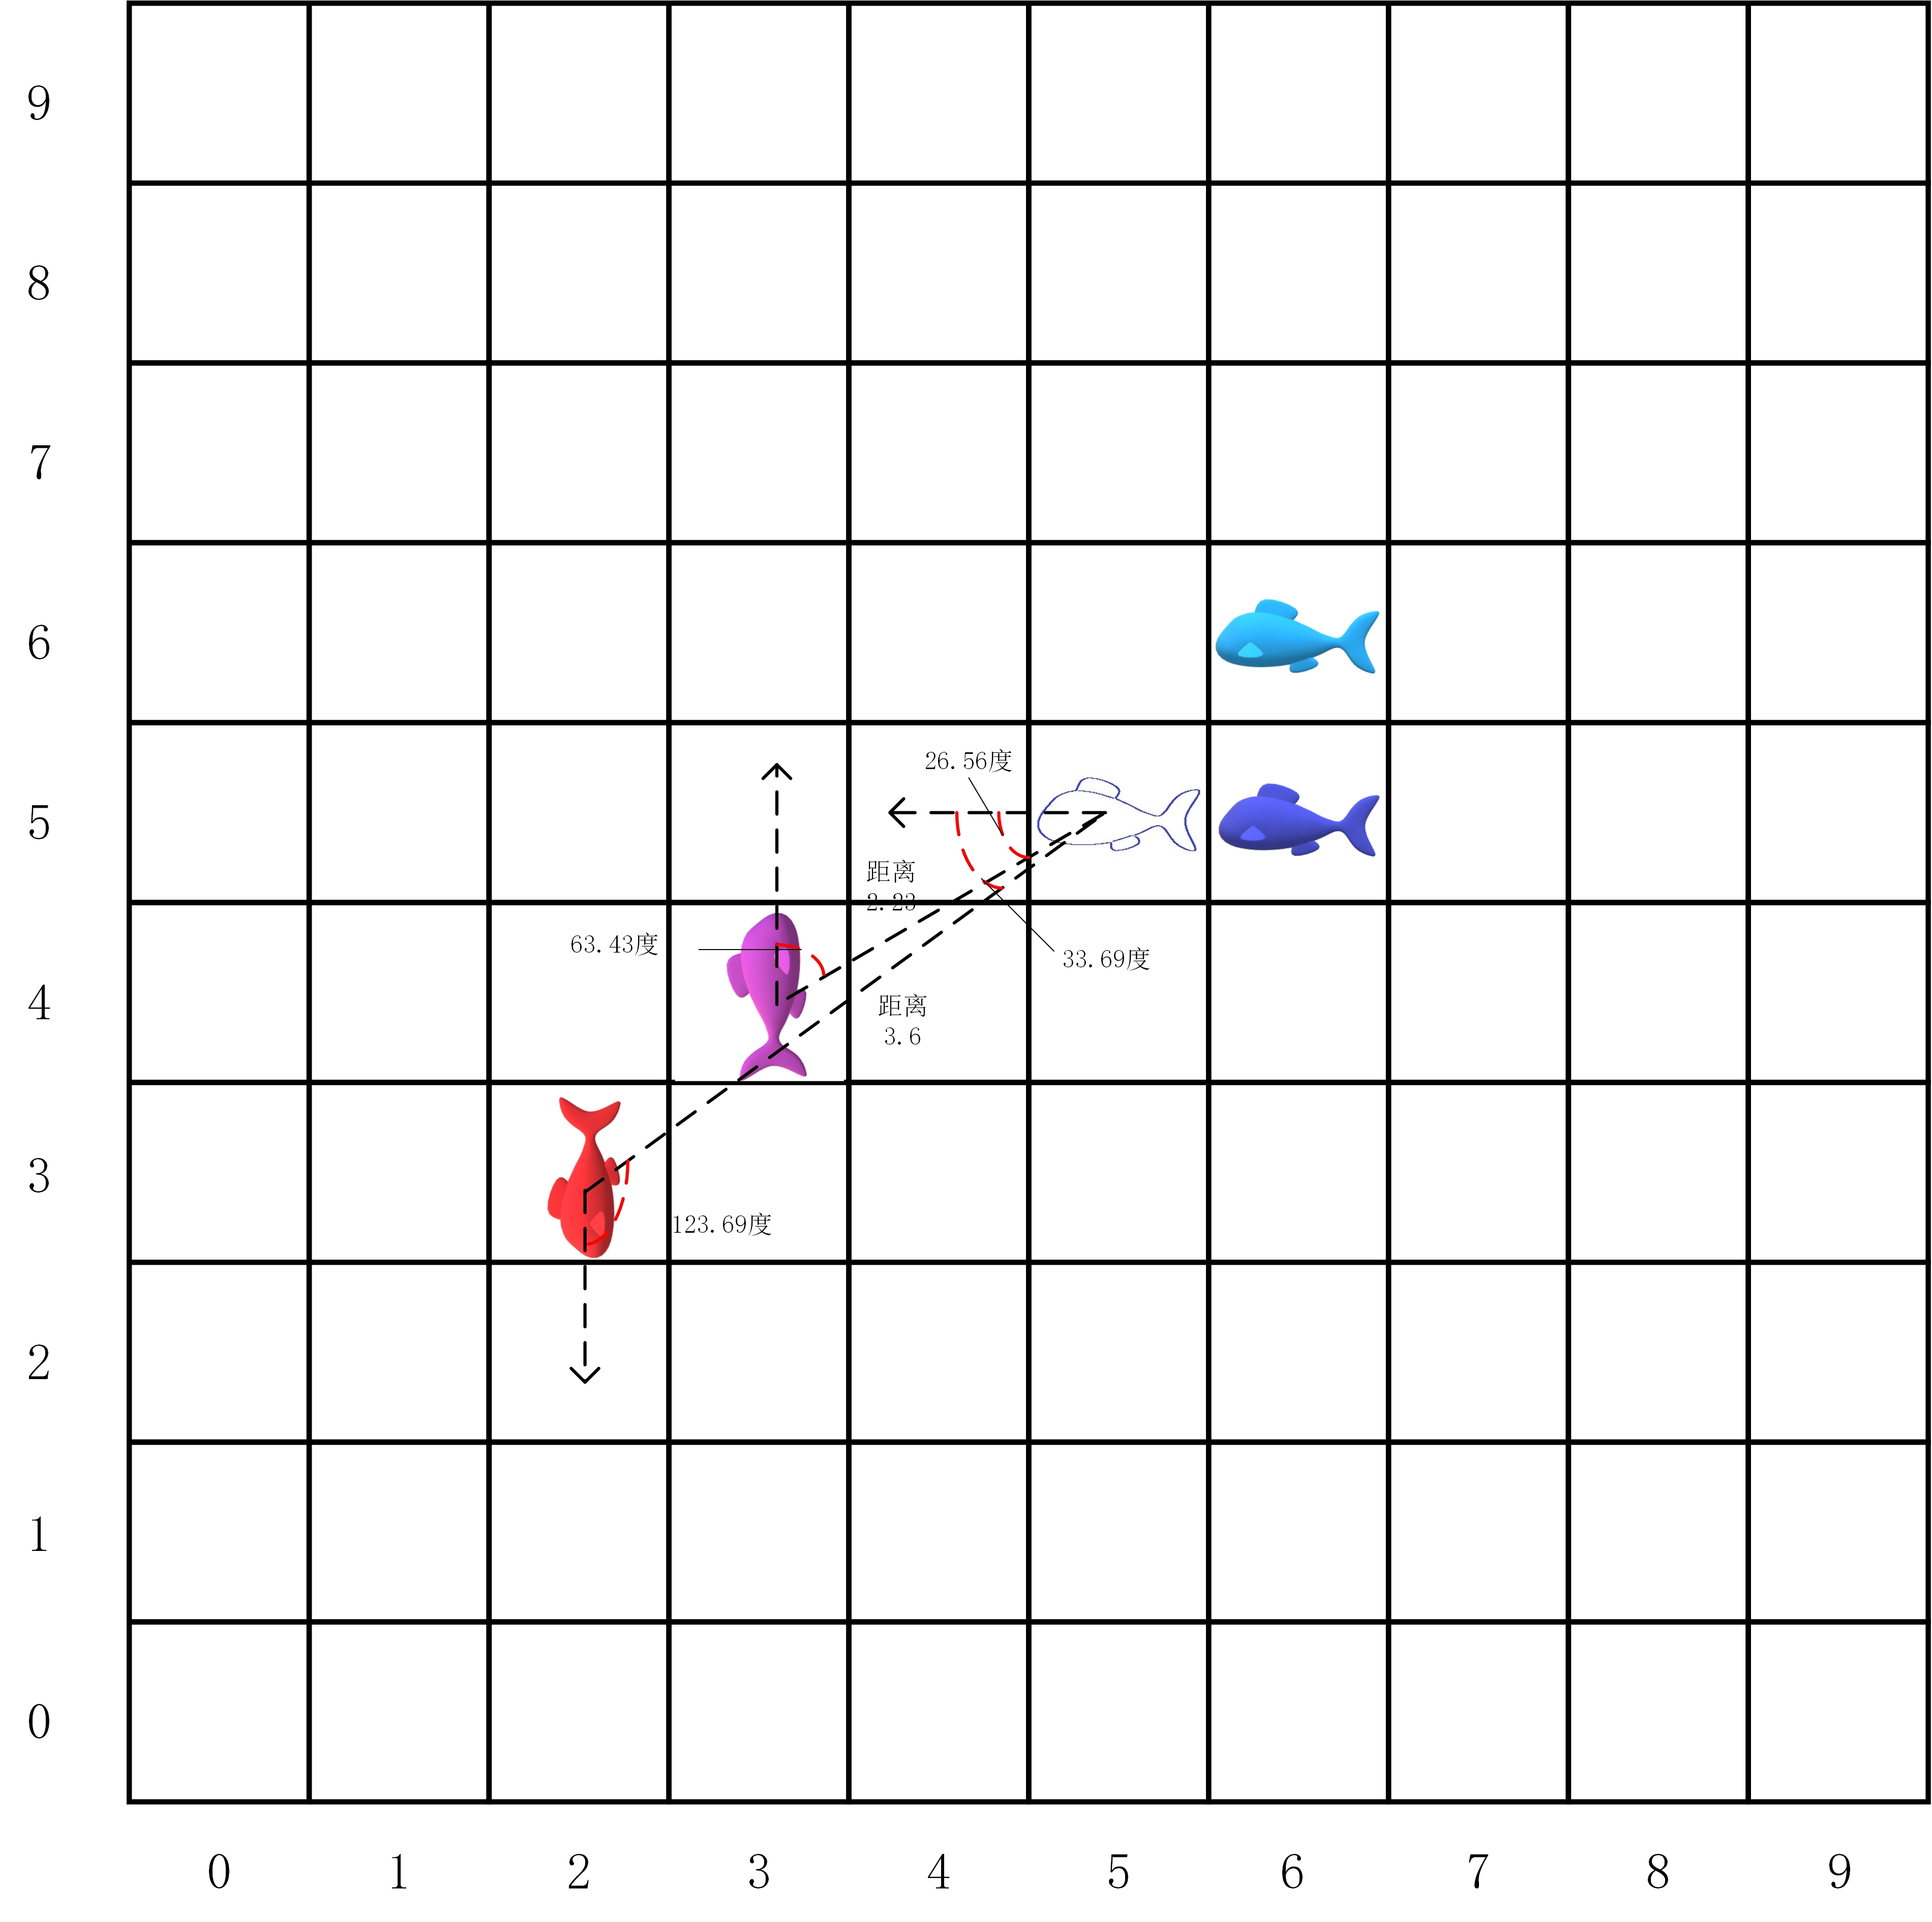
\includegraphics[width=0.45\hsize,height=0.45\hsize]{example/duoduiduo9.jpg}}
	\hspace{0.5em}
	\subcaptionbox{最终结果\label{fig3:duoduiduo:b}}
	{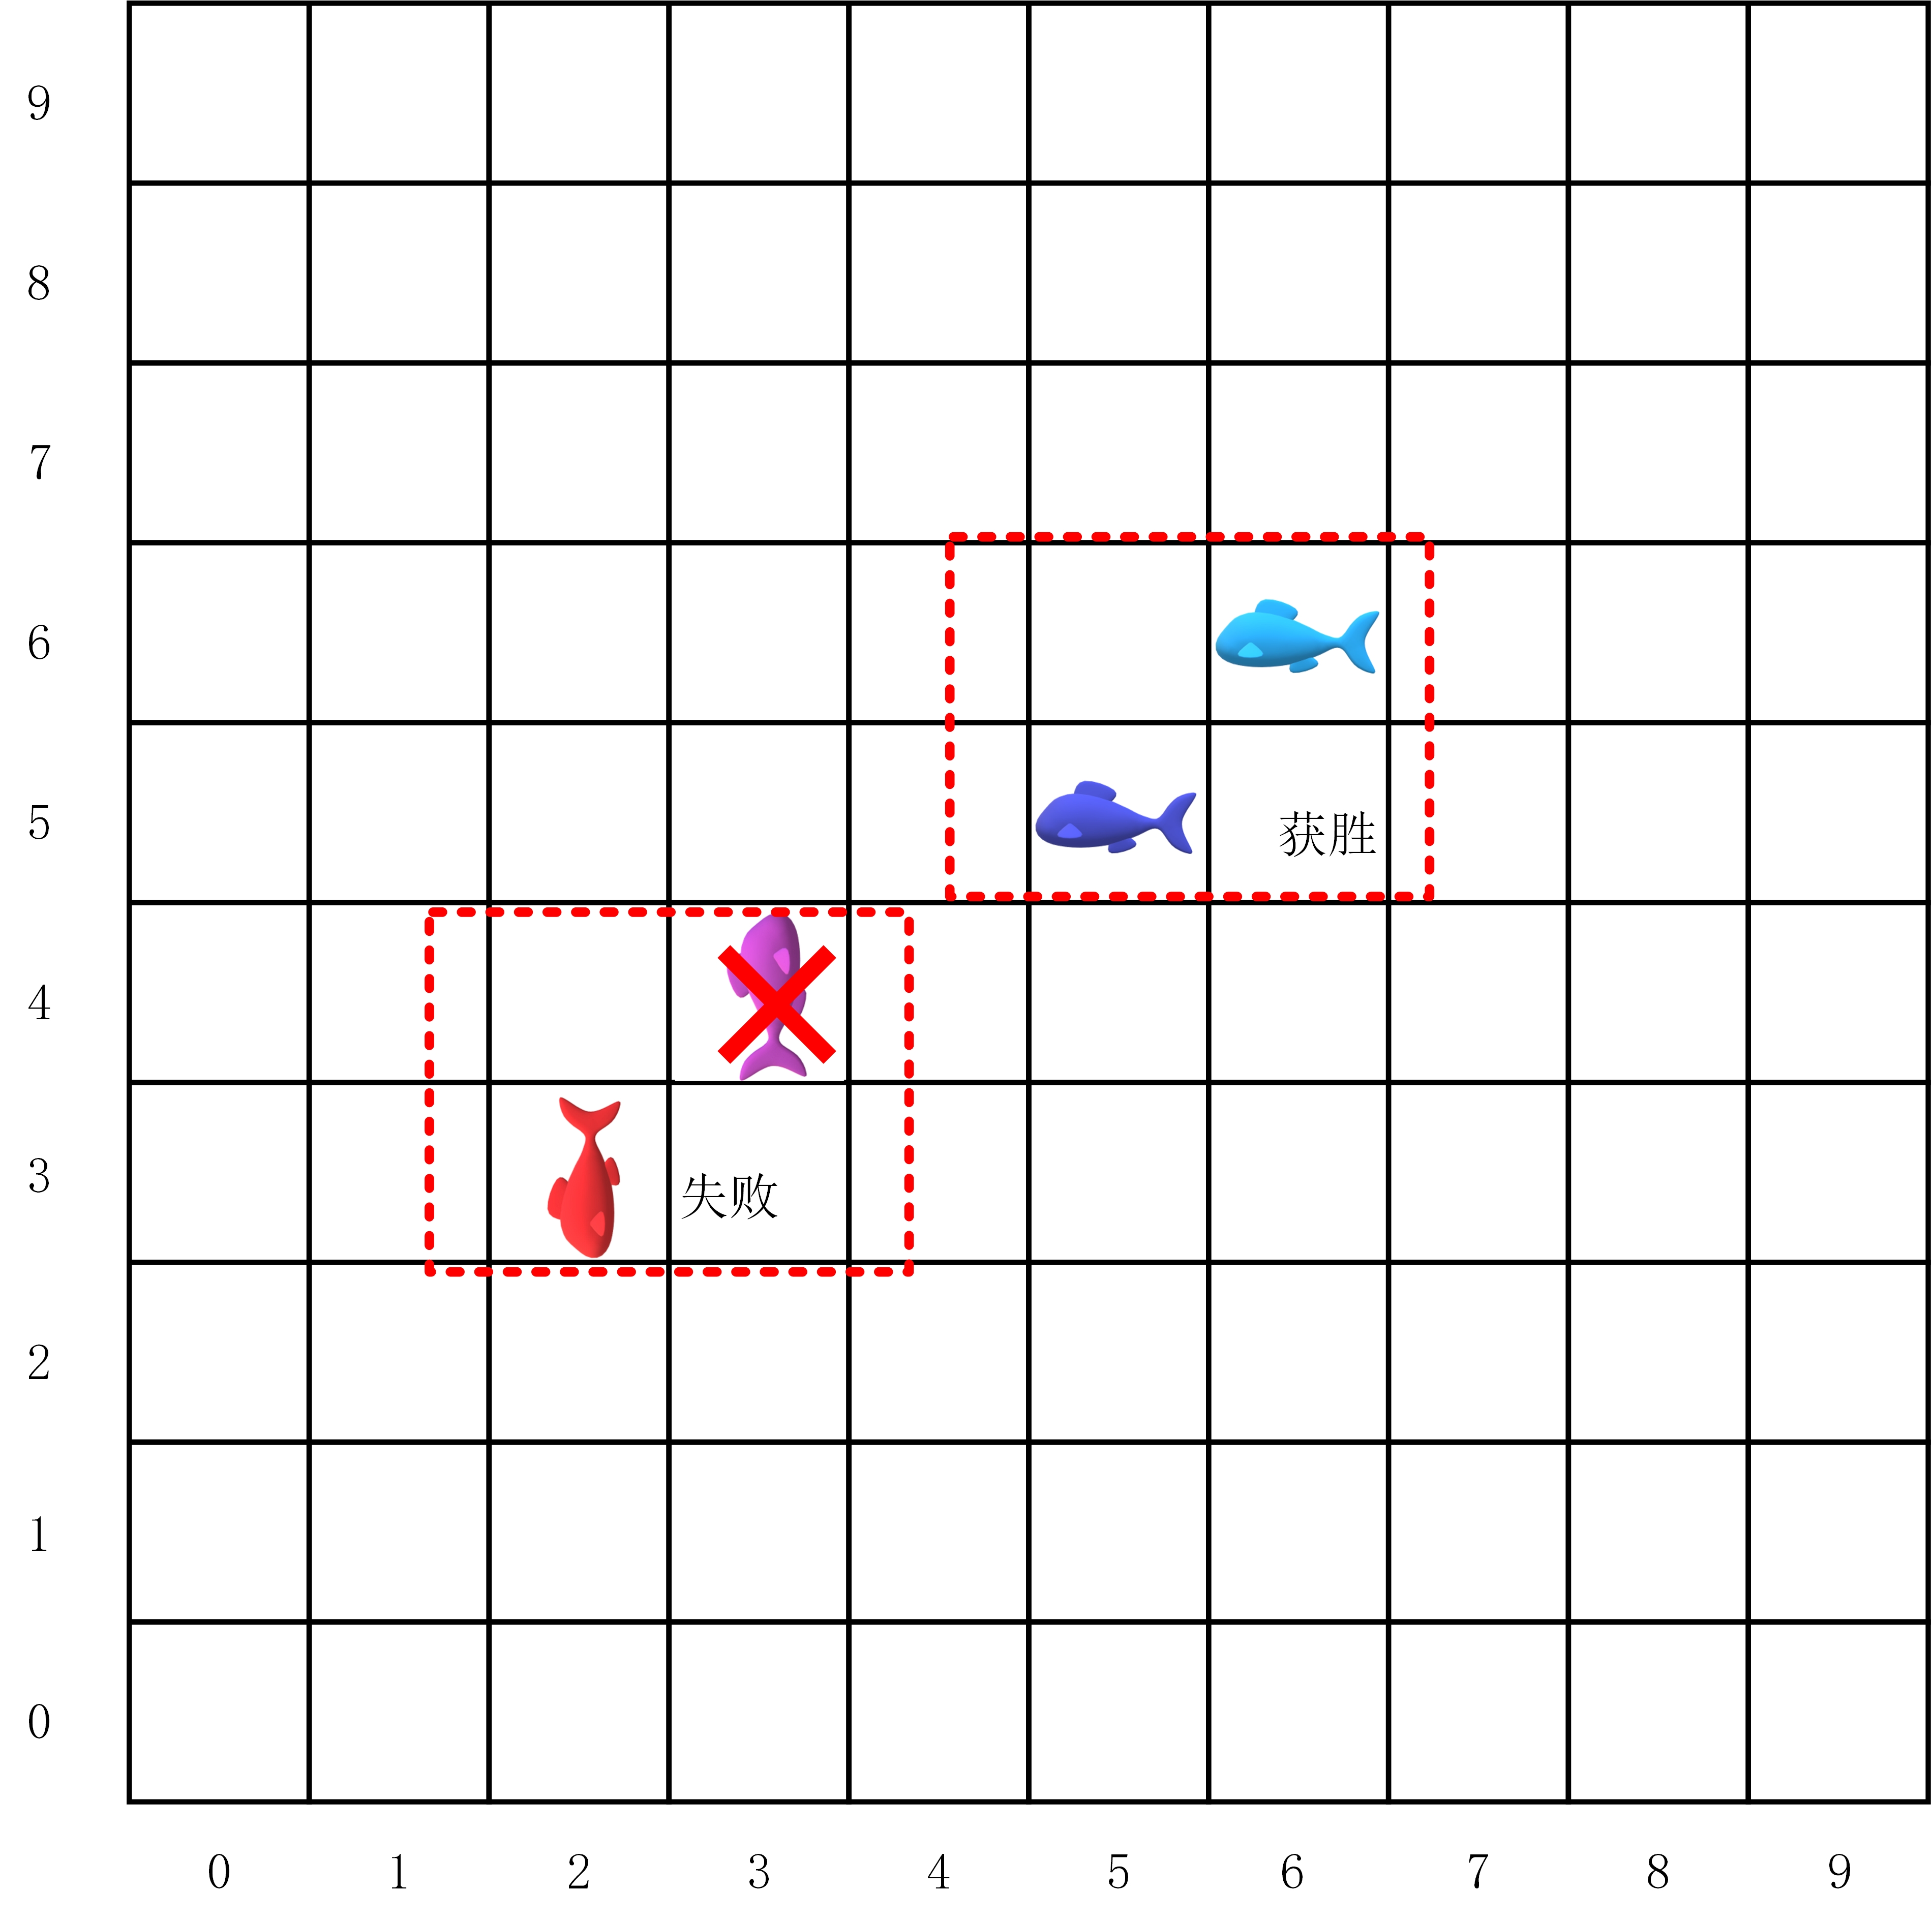
\includegraphics[width=0.45\hsize,height=0.45\hsize]{example/duoduiduo10.jpg}}
	\bicaption
	{多对多对弈状态分析}
	{Examples of response maps during occlusions and not.The first row shows the original and response maps with no occlusions while the second row shows the maps with occlusions. The first column are the shots of sequence bear front in Princeton dataset. The color response maps are in the second column while the depth’s are in the third.}
	\label{fig3:duoduiduo}
\end{figure}
可以看到最后粉色小鱼被吃掉,训练出来的模型具有一定的决策能力。在训练时需要合理平衡探索和利用的关系,在模型进行人机对抗时,采用贪婪策略选取概率最大的动作。利用从零开始学习模型的方案要比加入先验规则表现好,在模型前期可能会出现波动,但是在后期模型性能增长要比加入规则模型快。这也和由AlphaGo进化到AlphaZero得到的结果一致:在很多情况下利用人类专家数据学习的模型并不一定是最优的,让模型从白板开始训练,通过自我对弈进行能获得比人类认知更好的策略。
\section{本章小结}


